%% LyX 2.0.3 created this file.  For more info, see http://www.lyx.org/.
%% Do not edit unless you really know what you are doing.
\documentclass[twoside,english]{elsarticle}
\usepackage[T1]{fontenc}
\usepackage[latin9]{inputenc}
\pagestyle{headings}
\setlength{\parskip}{\smallskipamount}
\setlength{\parindent}{0pt}
\usepackage{array}
\usepackage{verbatim}
\usepackage{graphicx}

\makeatletter

%%%%%%%%%%%%%%%%%%%%%%%%%%%%%% LyX specific LaTeX commands.
%% Because html converters don't know tabularnewline
\providecommand{\tabularnewline}{\\}

%%%%%%%%%%%%%%%%%%%%%%%%%%%%%% User specified LaTeX commands.
% specify here the journal
\journal{}

% use this if you need line numbers
%\usepackage{lineno}

\makeatother

\usepackage{babel}
\begin{document}





\title{Predictive Quality Control}


\author[rvt]{C.V.~Radhakrishnan\fnref{fn1}\corref{cor1}\corref{cor2}}


\ead{cvr@river-valley.com}


\author[rvt,focal]{K.~Bazargan\fnref{fn2}}


\ead[url]{http://www.elsevier.com}


\fntext[fn1]{This is the specimen author footnote.}


\fntext[fn2]{Another author footnote, but a little more longer.}


\cortext[cor1]{Corresponding author}


\cortext[cor2]{Principal corresponding author}


\address[rvt]{River Valley Technologies, SJP Building, Cotton Hills, Trivandrum,
Kerala, India 695014}


\address[focal]{River Valleysfgs Technologies, 9, Browns Court, Kennford, Exeter,
United Kingdom}
\begin{abstract}
Abstract, should normally be not longer than 200 words. All work and
no play makes jack a dull boy. All work and no play makes jack a dull
boy. All work and no play makes jack a dull boy. All work and no play
makes jack a dull boy. All work and no play makes jack a dull boy.
All work and no play makes jack a dull boy. All work and no play makes
jack a dull boy. All work and no play makes jack a dull boy. All work
and no play makes jack a dull boy. All work and no play makes jack
a dull boy. All work and no play makes jack a dull boy. All work and
no play makes jack a dull boy. All work and no play makes jack a dull
boy. All work and no play makes jack a dull boy. All work and no play
makes jack a dull boy. All work and no play makes jack a dull boy.
All work and no play makes jack a dull boy. All work and no play makes
jack a dull boy. All work and no play makes jack a dull boy. All work
and no play makes jack a dull boy. All work and no play makes jack
a dull boy. All work and no play makes jack a dull boy. All work and
no play makes jack a dull boy. All work and no play makes jack a dull
boy. All work and no play makes jack a dull boy. All work and no play
makes jack a dull boy. All work and no play makes jack a dull boy.
All work and no play makes jack a dull boy. All work and no play makes
jack a dull boy. All work and no play makes jack a dull boy. All work
and no play makes jack a dull boy. All work and no play makes jack
a dull boy. All work and no play makes jack a dull boy. All work and
no play makes jack a dull boy. All work and no play makes jack a dull
boy. All work and no play makes jack a dull boy. All work and no play
makes jack a dull boy. All work and no play makes jack a dull boy.
All work and no play makes jack a dull boy. All work and no play makes
jack a dull boy. All work and no play makes jack a dull boy. All work
and no play makes jack a dull boy. All work and no play makes jack
a dull boy. \end{abstract}
\begin{keyword}
quadruple exiton \sep polariton \sep WGM \PACS 71.35.-y \sep 71.35.Lk
\sep 71.36.+c \MSC[2008]23-557
\end{keyword}
\maketitle



\section{Introduction}


\subsection{How is quality measured in present time?}

Present day quality measurements are done using various metrological
tools which quantify various shapes and/or form features of the part.
These features are given their individual limits by the designer which
help a metrologist in determining whether a part that has just been
manufactured is fit to be deemed a good part or not. However, most
of these tools are completely external equipments which need to be
explicitly used over the part(s) to see the results. This usually
calls for extra man-power and reduced throughput. So what manufacturers
end up doing is that they keep an inspection frequency for non critical
parts where quality checks on these parts are made at regular intervals
until one sees an anomaly. How this anomaly is responded to again
depends on what feature we are measuring.

The main problem with such a way of measurement is that :-
\begin{enumerate}
\item We have to make a compromise between the throughput and inspection
interval.
\item As the quality measurement is isolated from part manufacturing, you
can\textquoteright{}t detect a bad part unless it has already been
manufactured.
\end{enumerate}

\subsection{How do we propose to measure it?}

The main gist of the ideology we have applied is that, when a part
is being made, the information of each cut made by the machine is
reflected in some real-time aspect of the machine. It could be noise,
power, vibration, loads, etc. So what we do is, we record these variables
(in our case, power) real-time using appropriate tools and find a
correlation between these readings and the quality of the part manufactured.
This correlation can be tightened depending on the kind of accuracy
one is looking for. It also has an advantage over the conventional
approach in certain key aspects such as:-
\begin{enumerate}
\item The computational time is significantly less once a correlation model
has been made. Also, buying computational time is cheaper than wasting
producing time.
\item The feedback we get is near to real time and we could infact get early
warnings as the part is being made.
\item The kind of investment needed for this is much lesser compared to
buying precise instruments which, other than being pretty expensive,
usually have only a single functionality.
\end{enumerate}

\section{Methodology}


\subsection{\label{sub:Getting-Quality-data}Getting Quality data}

As we need to correlate between power readings during a producing
cycle and quality, we are essentially trying to create a model or
create a procedure to generate a model which would take the power
readings as input and give the quality as output. Thus, we needed
some input quality data for a training set.

For this, we monitored the Ra values of a part, which underwent turning
operation using a new tool insert, at regular intervals (once in 25
parts for first 500 cycles and once in every 10 parts from there on)
for 1030 parts. These measurements were made at two different faces
and three different locations in each face. We observed a downward
trend in the Ra values for the first 300 parts after which they were
more or less constant without any particular trend (save for an anomalous
jump at partt 500) till part 1000 after which they again rose up and
went outside the specification limit (see Fig \ref{fig:Quality-trend}).%
\begin{comment}
Insert graph. Metion new tool.
\end{comment}


\begin{figure}
\noindent \begin{centering}
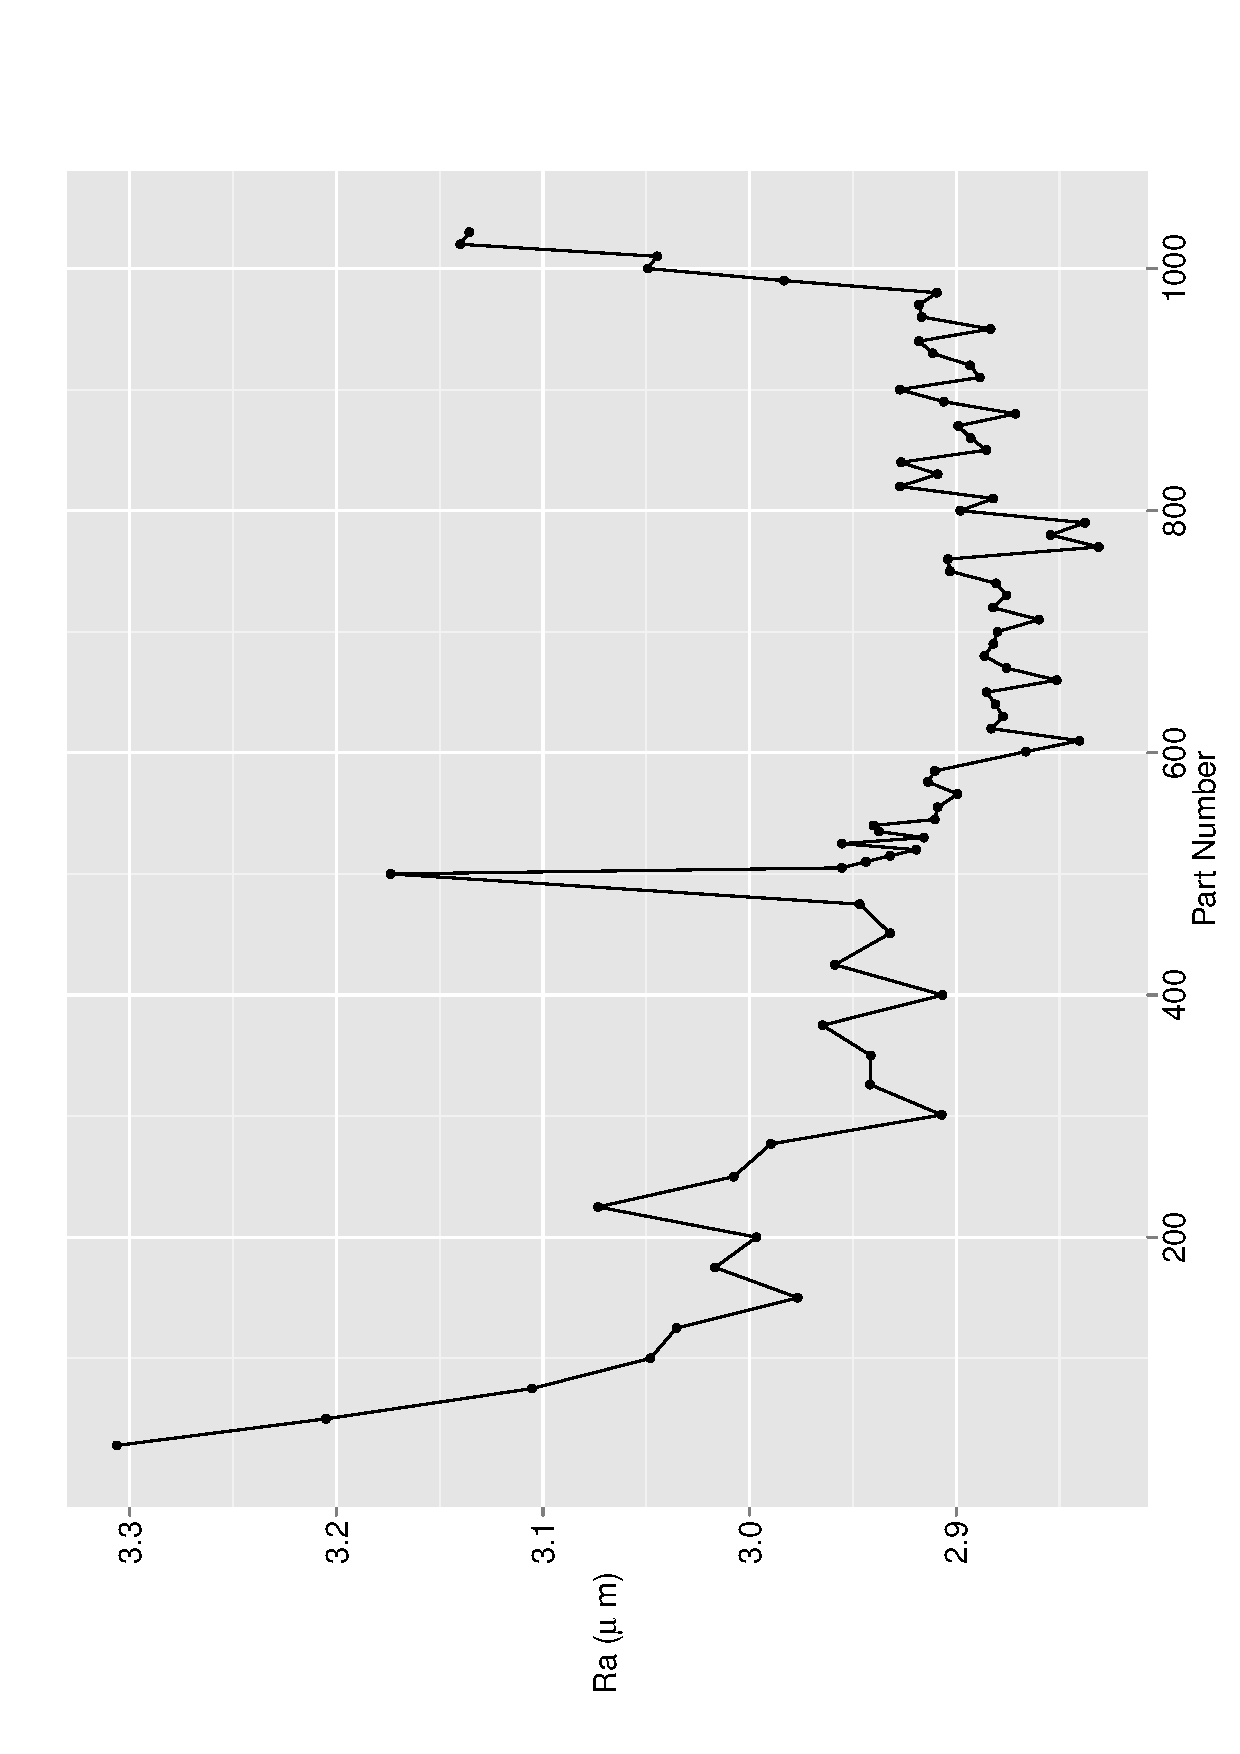
\includegraphics[width=14cm,height=8cm]{Images/qual_trend}
\par\end{centering}

\noindent \begin{centering}
\caption{Quality trend\label{fig:Quality-trend}}

\par\end{centering}

\end{figure}


So we decided to use the trend evident in the first 300 parts for
our model creation and verification. We created a 2 degree polynomial
fit for the first three hundred parts using 12 readings as our control
points.%
\begin{comment}
INSERT FIGURE AND POLYFIT STATS.
\end{comment}
{} The equation turns out to be 
\begin{equation}
y\approx3.35664-0.00324170.x+0.000006684611.x^{2}\label{eq:polyfit_1}
\end{equation}


Where, $y$ is the Ra value and $x$ is the part number. We see a
maximum error of $0.0833\mu m$ in the fit. For figure, see Fig.\ref{fig:Polynomial-fit-of Ra}
for the curve and Fig.\ref{fig:Residuals-of-polynomial_ra} for the
residuals' curve.

\begin{figure}
\noindent \centering{}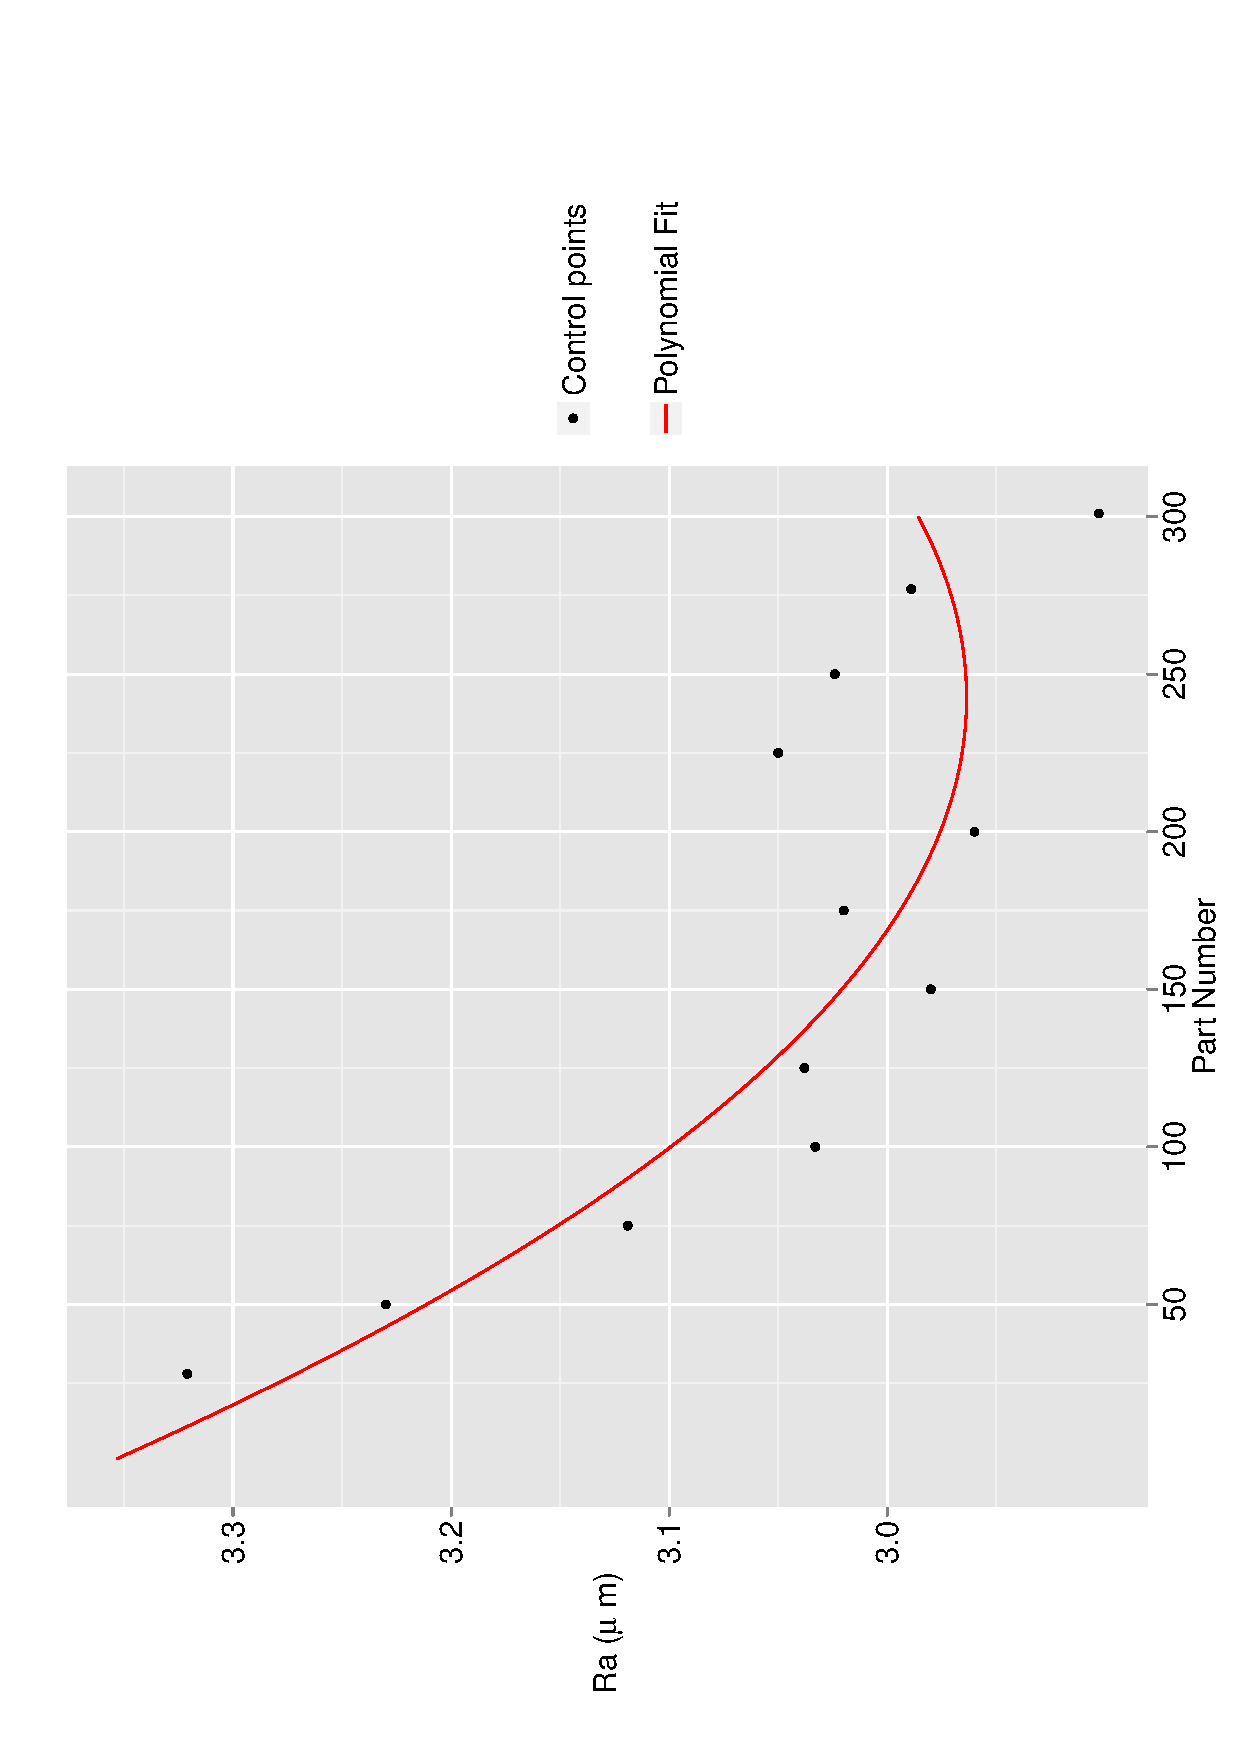
\includegraphics[clip,width=14cm,height=8cm]{Images/poly_fit_Ra}\caption{Polynomial fit of Ra values\label{fig:Polynomial-fit-of Ra}}
\end{figure}


\begin{figure}
\noindent \begin{centering}
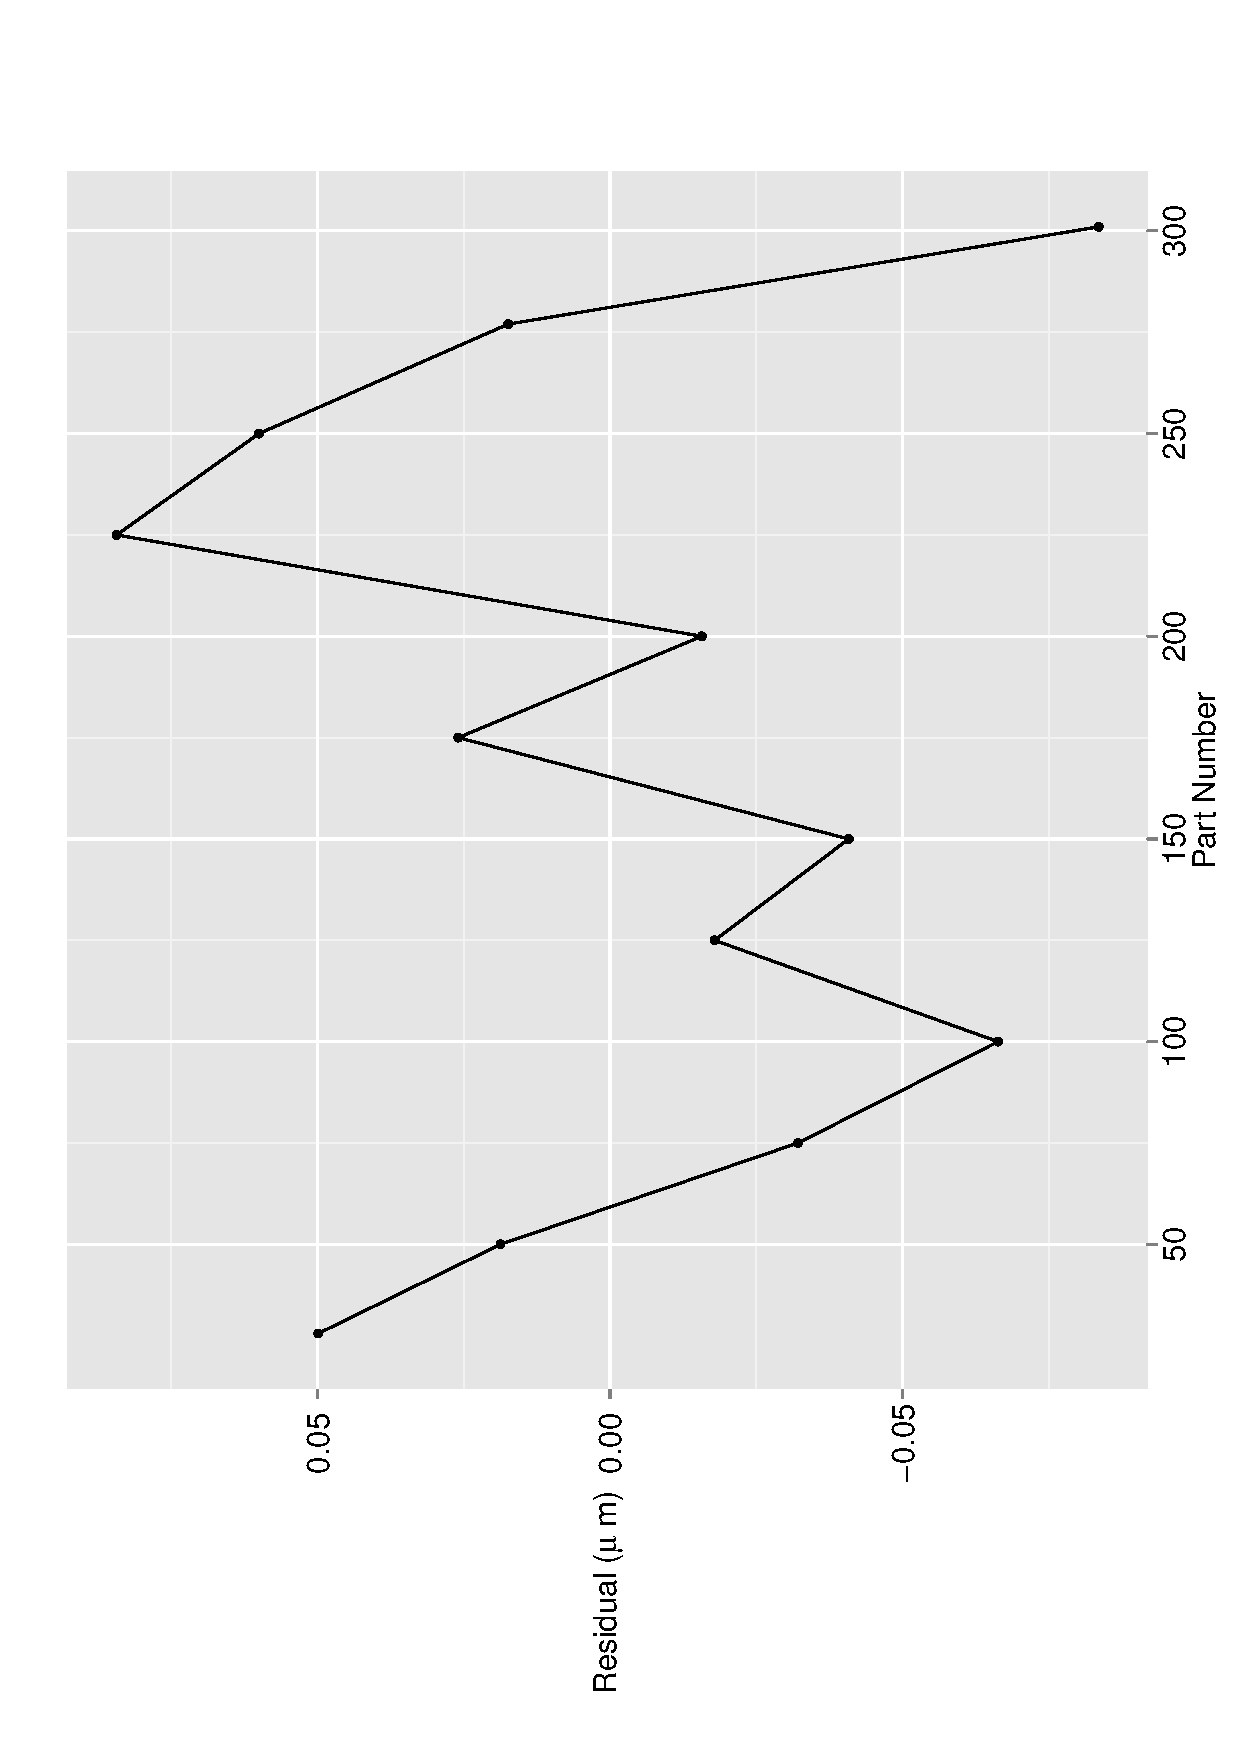
\includegraphics[width=14cm,height=8cm]{Images/poly_fit_residual}\caption{Residuals of polynomial fit for Ra values\label{fig:Residuals-of-polynomial_ra}}

\par\end{centering}

\end{figure}


Now this sample of 300 points was used as our quality data sample
which would be used for creating the model and verifying the same.


\subsection{Detect Cycles}

For input of the model we decided to use power readings. We decided
to go with power readings as one would expect a direct correlation
between energy consumed and material removed. Also, it depends very
little on parts of the machine which are not responsible for cutting
(eg. housing) and thus we can make our system more flexible for varioua
machines. Also, power readings can be easily obtained using conventional
power meters.

As we plan to make an autonomous correlation model, we need to be
able to correctly identify the start and end times of a production
cycle. In relatively newer machines, this data can be obtained via
the controller. However, the number of machines which are not capable
of that are quite large. So we need to come up with a method to let
the machine identify a cycle and record its start and end time. We
use a simple pattern matching approach here. We are going to analyze
the power readings we get as a stream of data and in it look for recognisable
patterns which would indicate whether and where a cycle occurred.
So to start, we need a known producing cycle which we can use as a
template for comparisons. Once we decide this template we use an algorithm
called \textbf{Dynamic Time Warping} (DTW).


\subsubsection{Dynamic Time Warping}

Dynamic time warping is a method to compute the similarity between
two sequences. To compare these two sequences, one can \emph{warp
}(stretch/compress) the sequences non-linearly. Originally used as
a tool to detect speech patterns in \emph{Autonomous speech recognition,
}DTW is now used in many applications which need to compare one sequence
to another. One can limit the amount of warping and thus ensure that
realistic results are obtained.%
\begin{comment}
INSERT A MATCHED FIGURE.
\end{comment}


\begin{figure}
\noindent \begin{centering}
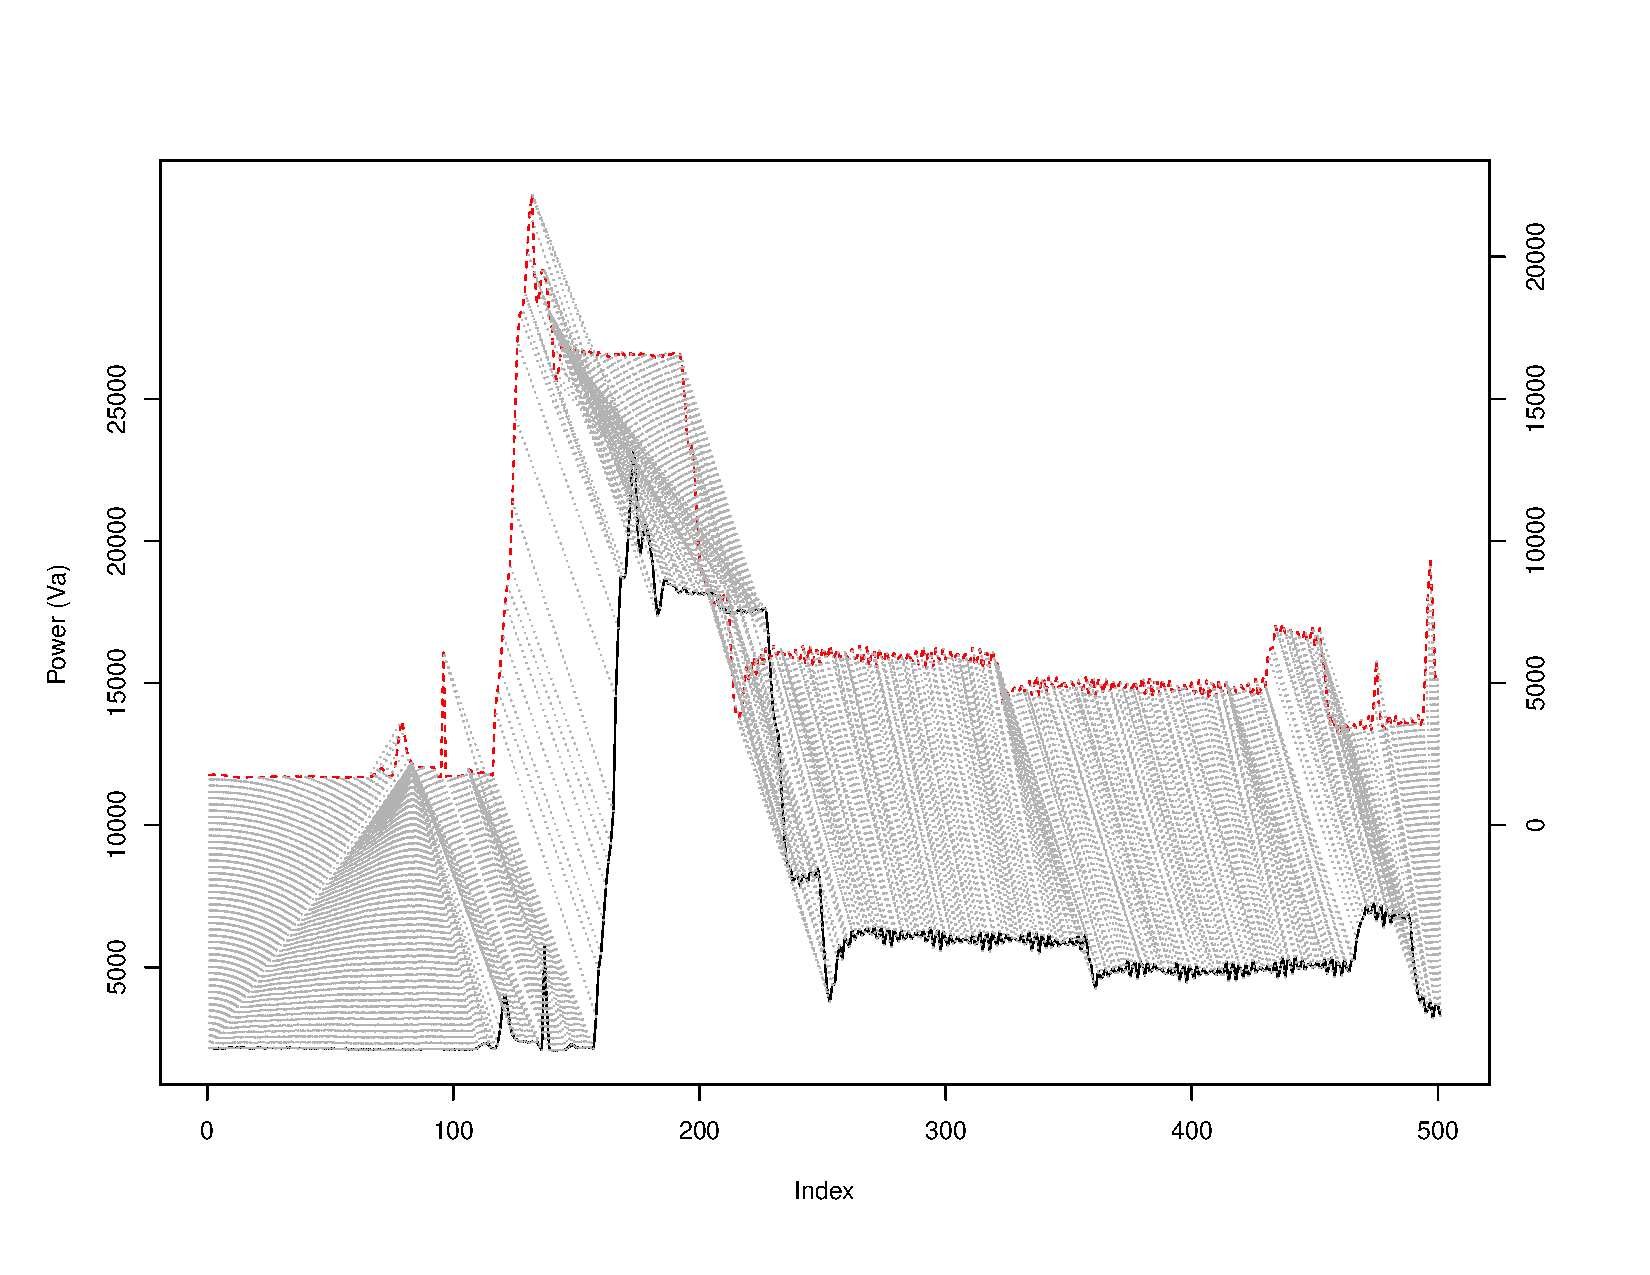
\includegraphics[width=14cm,height=11cm]{Images/dtw_match}\caption{Mapping of two time streams using DTW\label{fig:dtw fig}}

\par\end{centering}

\end{figure}


As we can see in Fig \ref{fig:dtw fig}, even if we have a time shift
and small variations in data, the DTW algorithm maps significant features
appropriately. This robustness is a result of the warping along time
direction allowed. One can also limit the amount of warping permissible
so that we can ensure that only physically possible cases are deemed
similar. The distance between two sequences being compared is found
has sum of distances (euclidean, manhattan, etc) between these mapped
points.


\subsection{Extracting input from power consumption pattern}

\noindent Now we have the start and end times for 300 producing cycles
and we can use this data to get power consumption patterns for each
individual part and use it as necessary. However, we can't use these
patterns directly as inputs for any machine learning algorithm as
it has many inherent problems. The main reason being that small time
offsets in the time series data could throw off the result by a large
amount. So we basically needed to process our power pattern to extract
more stable information from it. By stable, we mainly mean that we
must get same information if we shift a cycle by a small amount (say
1 sec). However in the process of making it stable, we also have to
make sure that we don\textquoteright{}t lose the individuality of
the pattern as we depend on this individual character for our quality
reading. We resolved this using two methods:-
\begin{enumerate}
\item Scalar extractions from pattern.
\item Cycle splitting.
\end{enumerate}

\subsubsection{Scalar extractions from splitting}

Here we extract from our cycle a set of scalars which are stable and
do not get affected due to small changes like minor time scaling,
peaks,etc. These scalars could be mean, standard deviation, DTW distance,
median, mode, amplitude, etc. However, as pointed out earlier, using
these scalars alone would render many cycles to be same as we are
wasting a lot of information. So we use, not one, but a combination
of these scalars as now we get more options of variability thus giving
us our desired result of stable and unique inputs. Here, we used only
two of these functions:-
\begin{enumerate}
\item Mean
\item Standard deviation
\end{enumerate}

\subsubsection{\label{sub:Cycle-splitting}Cycle splitting}

This is a much more important process and increases the effectiveness
of scalar extraction. What we essentially do cut the cycle into a
number of parts using different methods (which will be discussed later)
and apply the scalar extraction for each segment. So now we increase
our number of inputs and also increase the individuality of each input
in a stable way. The combination of various scalars for all splits
of a cycle represent a particular cycle and all of them are used to
get a final quality parameter (in our case, Ra) for each cycle. These
\emph{predicted quality metrics }can be compared against our \emph{experimental
quality metric }and we can get error associated with each part.

Much more importantly, when we later analyze our results, we can actually
pinpoint which segments of the cycle are primarily responsible for
the quality parameter being measured (in our case, Ra). This kind
of information can prove to be really useful as now we can know what
part of the cycle is primarily responsible for which quality parameter.
This can in turn help us detecting tool damages when we observe a
deviation in certain quality parameter. Splitting the cycle gives
us one more important advantage. Now we can calculate the quality
metric of a cycle by including one split at a time, into our input
set, sequentially. This can be really helpful in predicting parameter
qualities before the machining is over and thus can help us in taking
corrective action.

We primarily employed four different methods to split cycles. They
were:-%
\begin{comment}
Insert figures
\end{comment}

\begin{enumerate}
\item \textbf{Uniform splitting}: As the name suggests, we split the cycle
into equally sized sections. The number of parts would depend on how
much accuracy we want and how much computation cost we can afford
(Fig \ref{fig:Uniform-splitting}).
\begin{figure}
\noindent \centering{}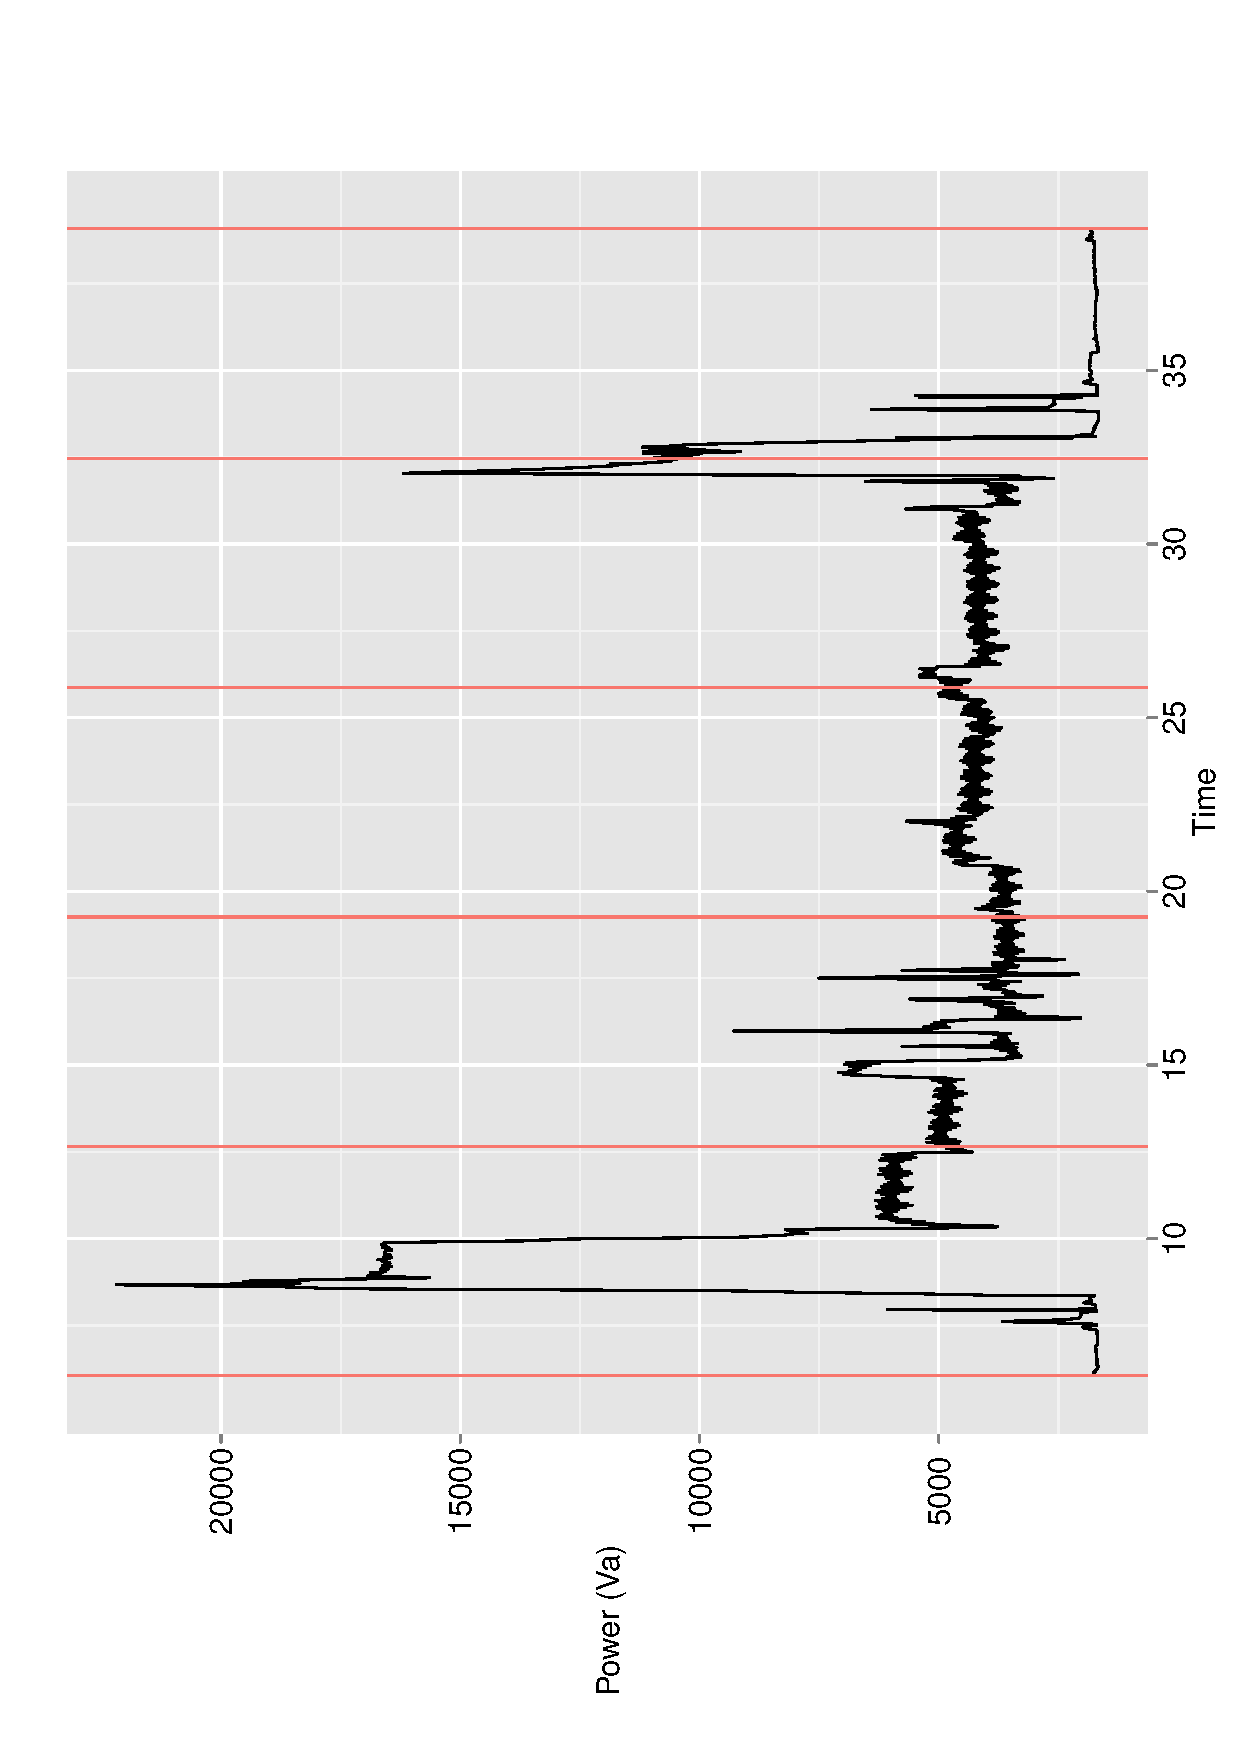
\includegraphics[width=14cm,height=8cm]{Images/uniform_split}\caption{Uniform splitting (5 sections)\label{fig:Uniform-splitting}}
\end{figure}

\item \textbf{Forward feedback splitting}: In this, we first assume the
entire cycle to be a single section and run our algorithm (which is
explained in \ref{sub:Model-Selection} and \ref{sub:Model-Creation})
to select a model. Then we find the RMSE of the best available solution
for the test set. Now we split the cycle into two equal halves and
again run the algorithm and get a new RMSE. If the relative drop in
RMSE is higher than a threshold and the timespans of newly created
splits is longer than a user-defined limit, we retain the split and
move to the first half which we split and continue comparing and splitting
it further. However, if the improvement is not significant enough,
we move on to the next available section and continue till we are
done with all the sections. It is slightly biased to create more cuts
in the beginning of the cycle as we approach the limits of numerical
accuracy of the model after the first few cuts (Fig \ref{fig:Forward-feedback-splitting}).
\begin{figure}
\noindent \begin{centering}
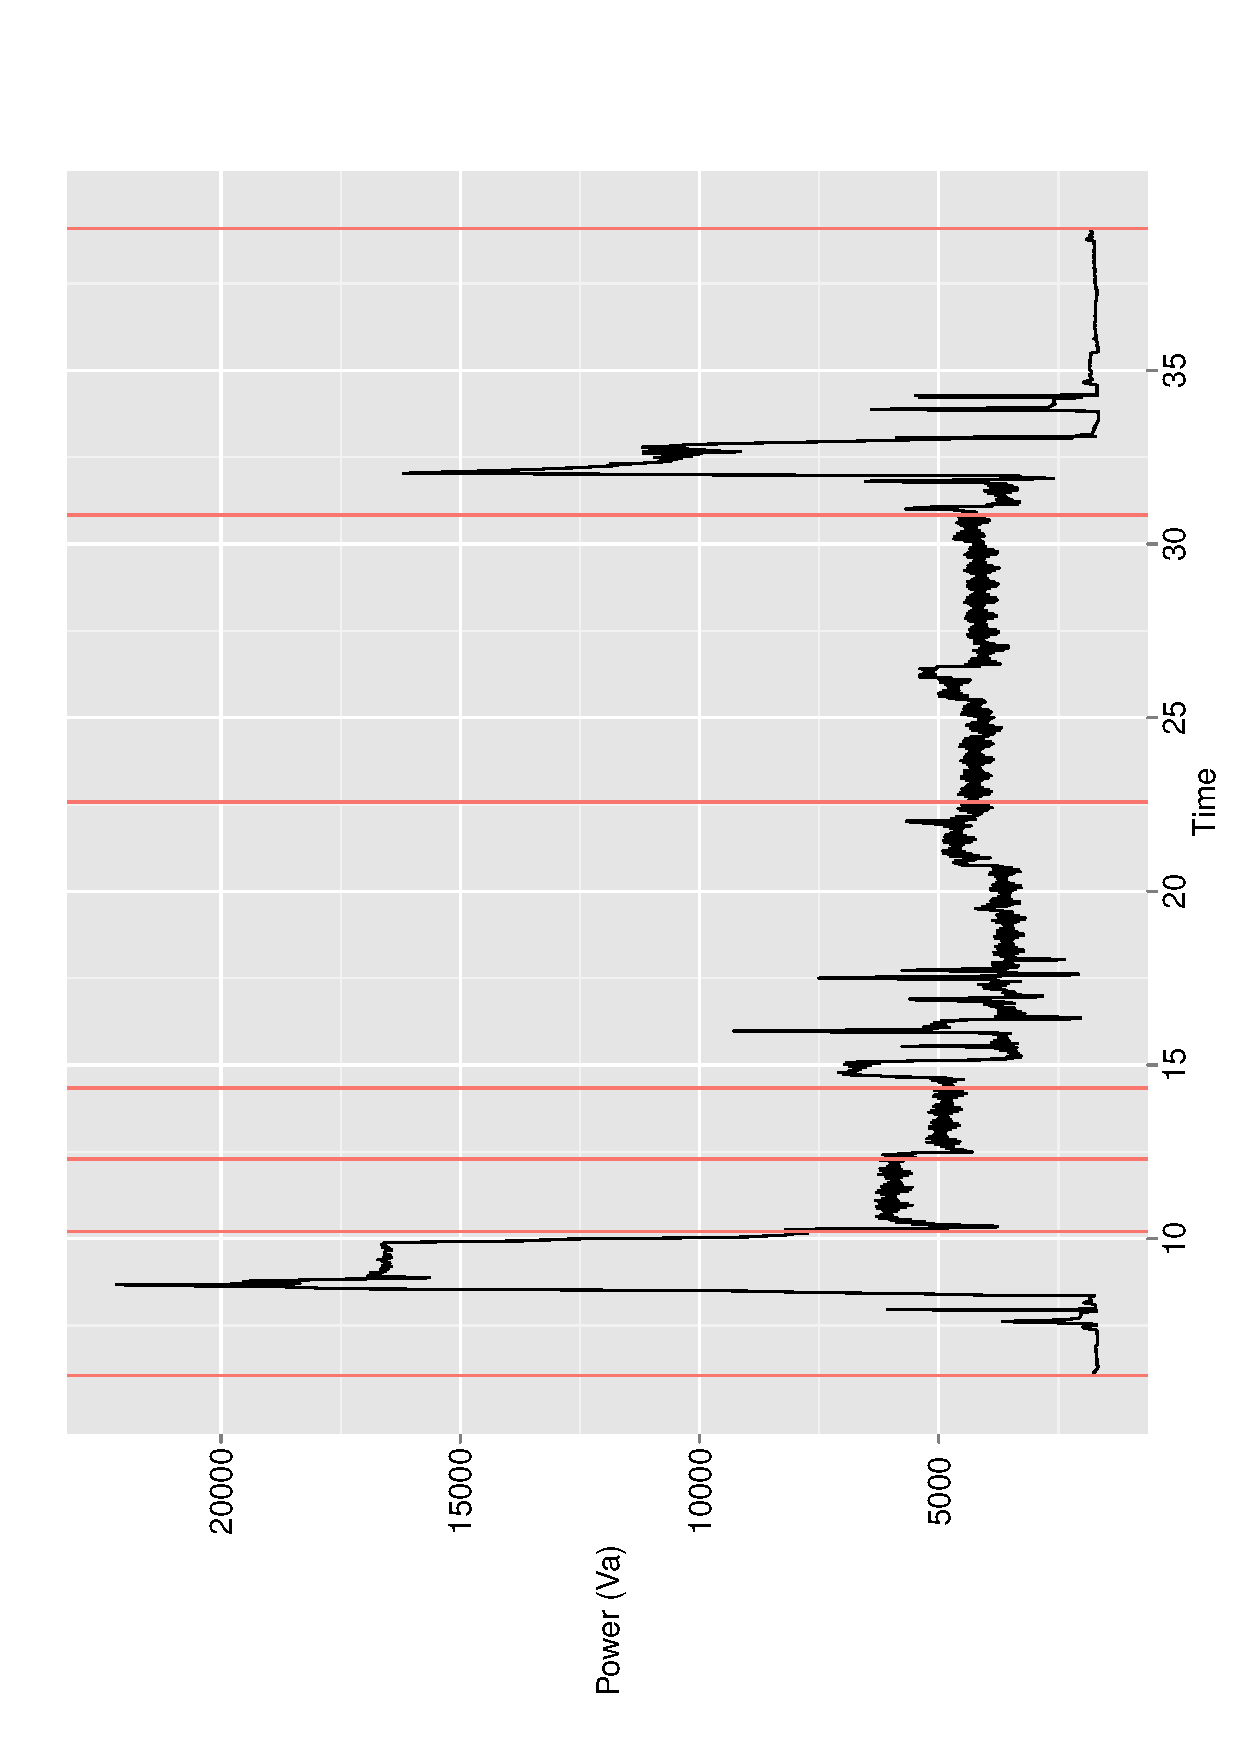
\includegraphics[width=14cm,height=8cm]{Images/forward_split}
\par\end{centering}

\noindent \centering{}\caption{Forward feedback splitting\label{fig:Forward-feedback-splitting}}
\end{figure}

\item \textbf{Reverse feedback splitting}: This is almost like the Forward
Feedback Splitting but instead of biasing cuts to the start, this
one biases cuts to the end as one moves to the latter half after a
succesful split has been made and moves to preceding sections in case
of unsuccesful (which are either very short or don't give significant
improvemetn in RMSE) splits (\ref{fig:Reverse-Feedback-splitting}).
\begin{figure}
\noindent \begin{centering}
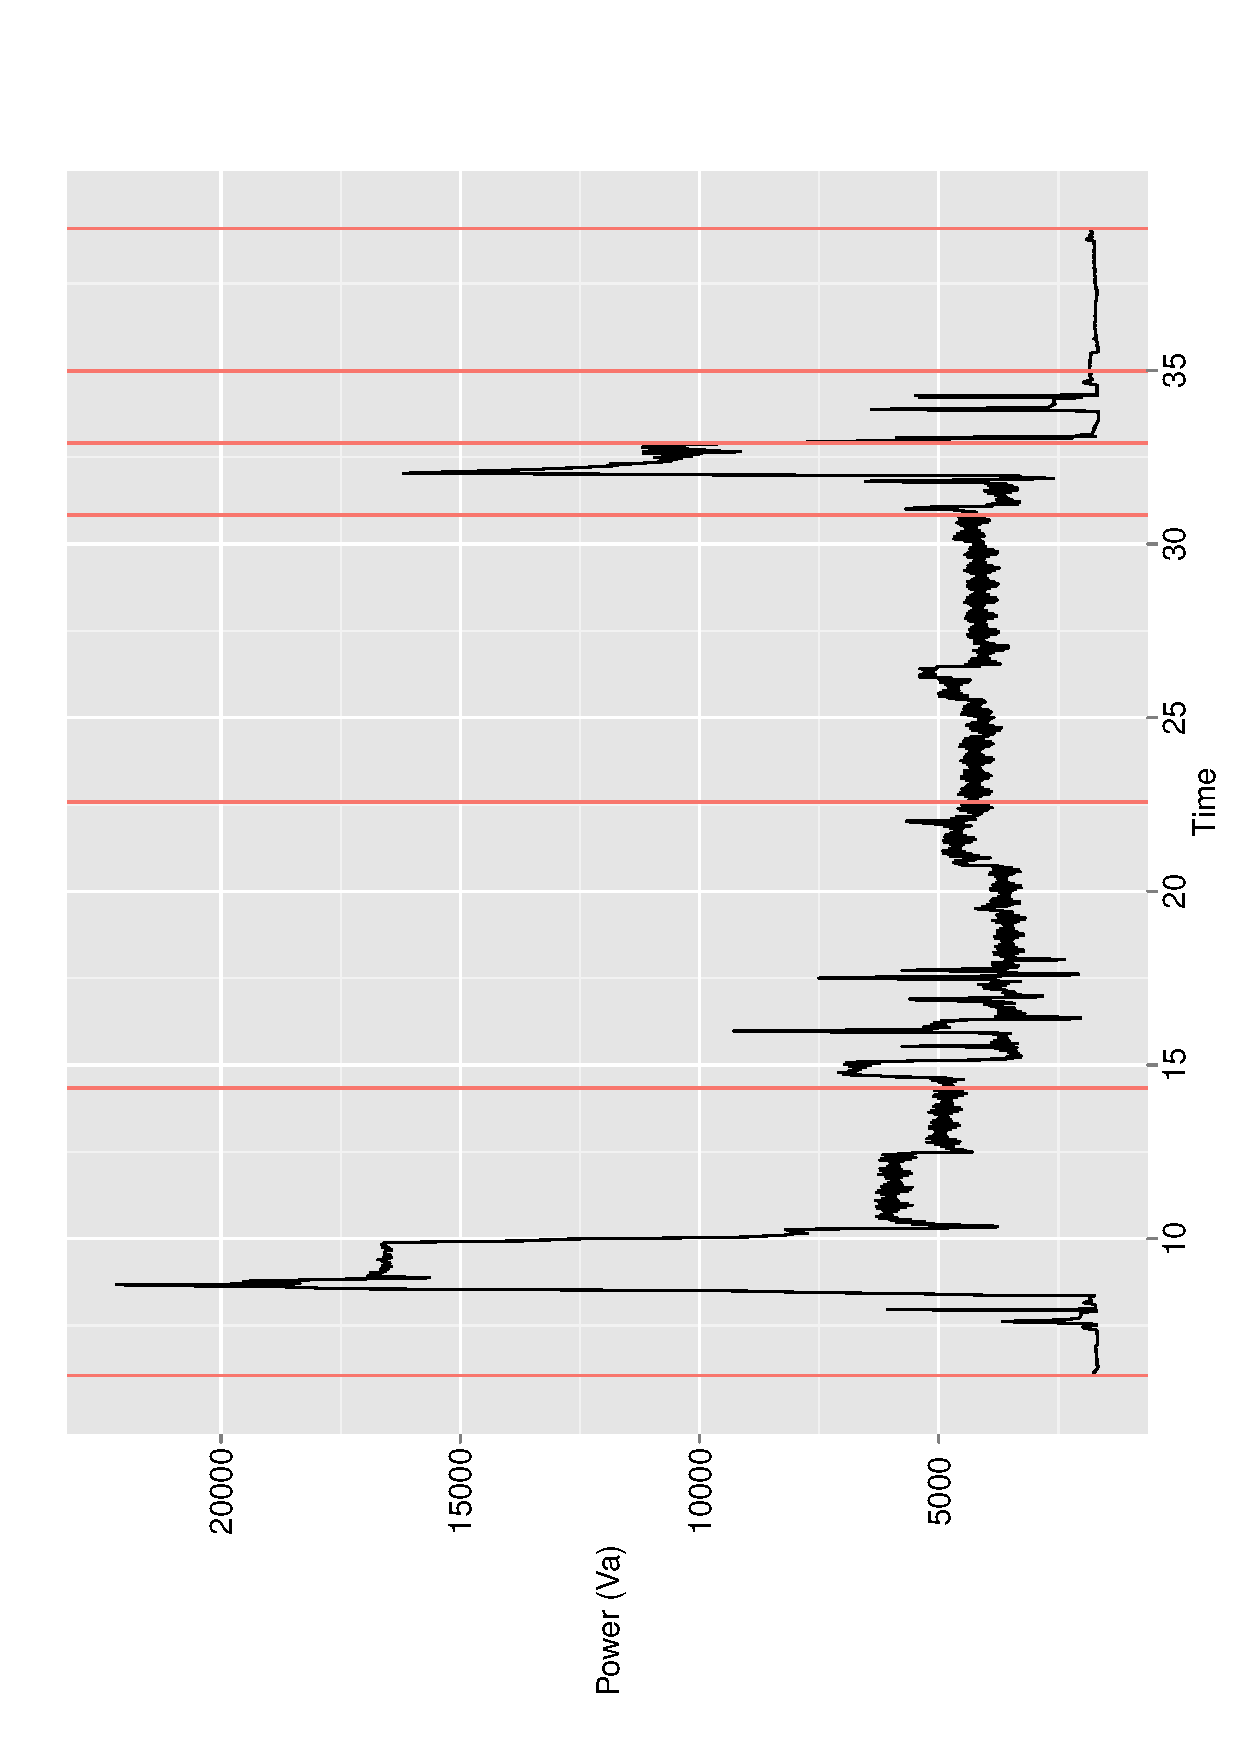
\includegraphics[width=14cm,height=8cm]{Images/reverse_split}
\par\end{centering}

\noindent \centering{}\caption{Reverse Feedback splitting\label{fig:Reverse-Feedback-splitting}}
\end{figure}

\item \textbf{Phase dependent splits}: These are cuts which signify a change
in process in the machining. Theoretically, these should be the most
optimum cuts as they point towards specific process. However, finding
them out autonomously can be tricky if wanted for all situations thus
these cuts have to be entered manually (Fig \ref{fig:Phase-dependent-split}).
\begin{figure}
\noindent \begin{centering}
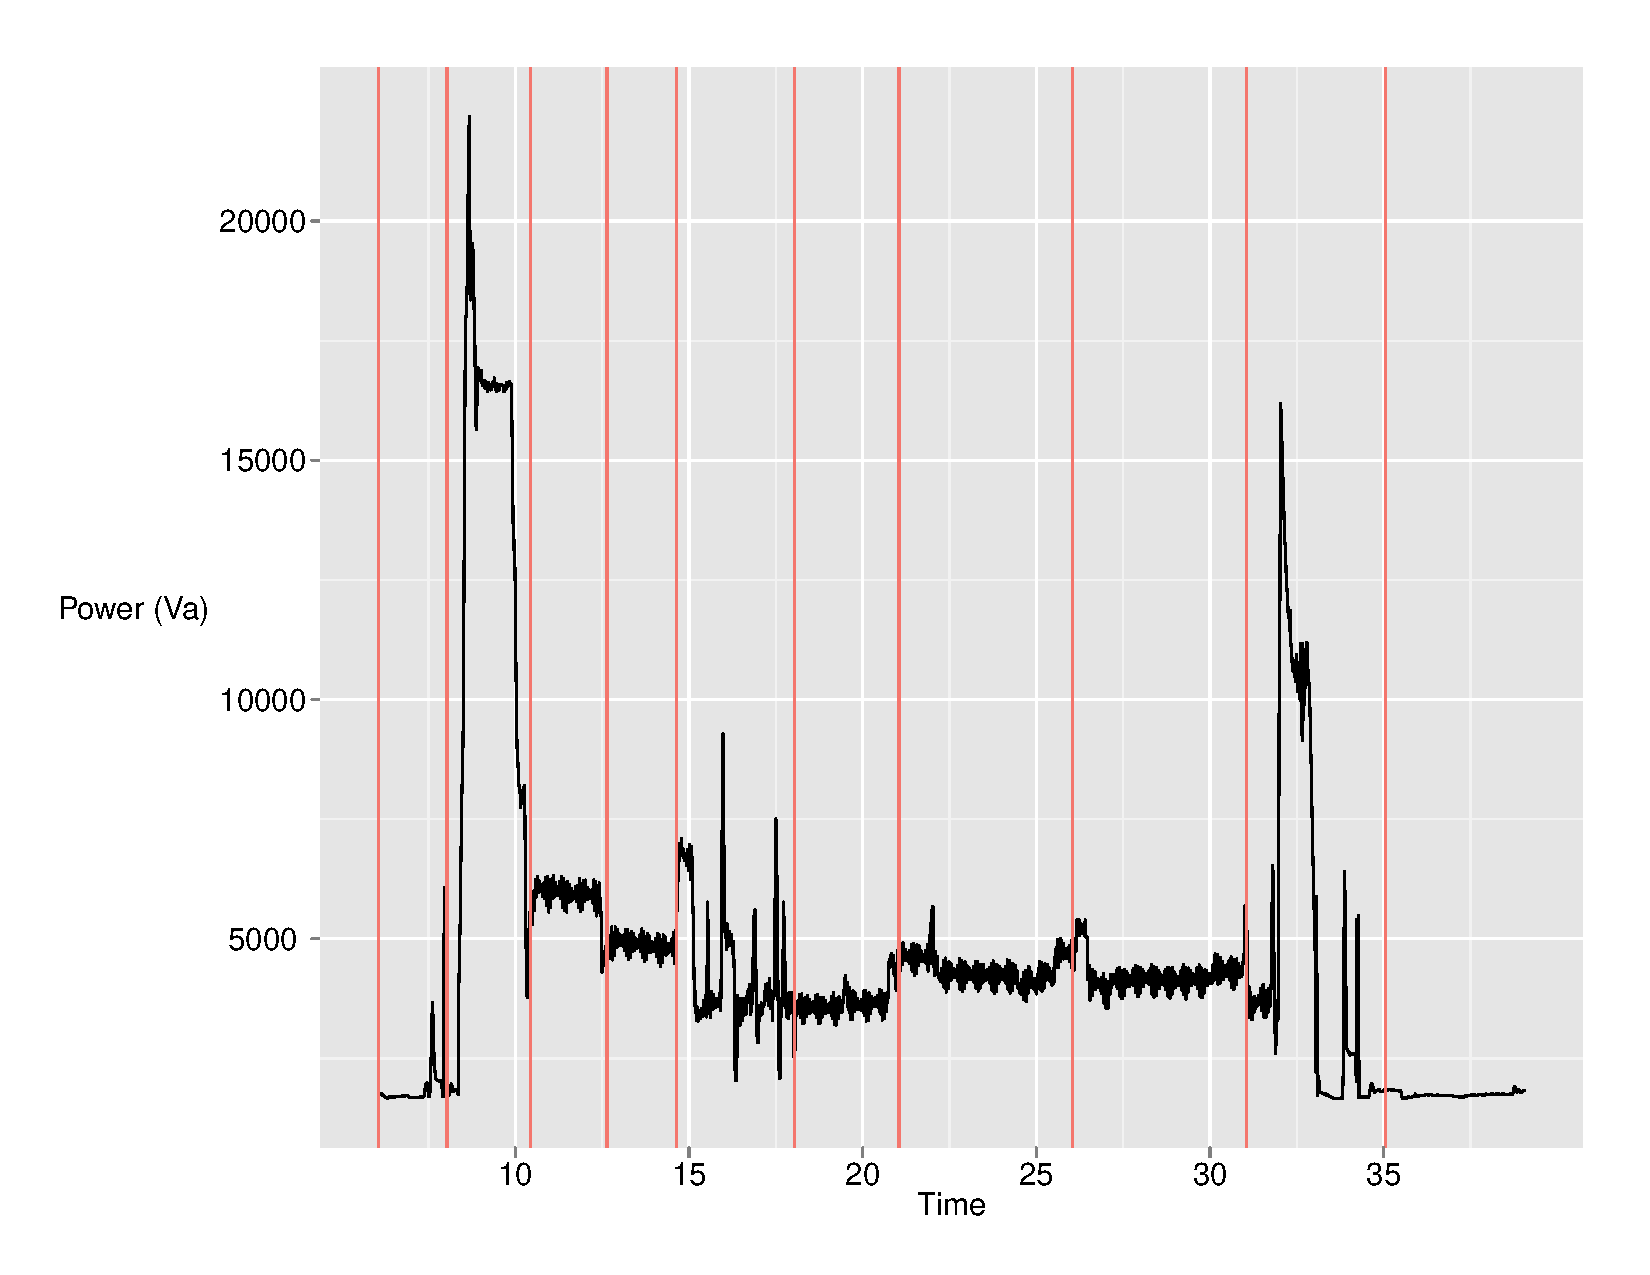
\includegraphics[width=14cm,height=8cm]{Images/manual_split}
\par\end{centering}

\noindent \centering{}\caption{Phase dependent split\label{fig:Phase-dependent-split}}
\end{figure}

\end{enumerate}
Now, after splitting the cycle appropriately and using scalar extraction
for each split, we have a bunch of variables for a cycle which we
will later use to get a wider set of data.


\subsection{\label{sub:Model-Selection}Model Selection}

There are a plethora%
\begin{comment}
CHECK IF THERE ACTUALLY ARE A PLETHORA OF METHODS
\end{comment}
{} of machine learning algorithms which we could use to establish a
relation between our input and output. We decided to try the very
simple models and thus decided to use \emph{Polynomial Regression.}
However, as our number of variables were bound to be high, we decided
to keep the model complexity to a minimum and thus decided to go forward
with \emph{Regularised Polynomial Regression.}


\subsubsection{Regularised Regression}

Say we try to create a linear relation between input variables$x_{1},x_{2},x_{3}....,x_{n}$and
output variable $y.$As it is linear, we can assume our equation to
be
\begin{equation}
y=a_{0+}a_{1}x_{1}+a_{2}x_{2}+a_{3}x_{3}.......+a_{n}x_{n}\label{eq:regul 1}
\end{equation}


Where $a_{1},a_{2},a_{3}.......a_{n}$ are the coefficients which
we have to find. 

Let us define input variable $\mathbf{X}$ and $\mathbf{A}$ as 
\begin{equation}
\mathbf{X_{i}=}(x_{1,}^{i}x_{2}^{i},x_{3}^{i},......,x_{n}^{i})\label{eq:regul 2}
\end{equation}


\begin{equation}
\mathbf{A}=(a_{1},a_{2},a_{3},.....,a_{n})\label{eq:regul 3}
\end{equation}


where $x_{j}^{i}$ is the $i^{th}$ instance of the $j^{th}$ variable.
Thus, we get
\begin{equation}
y_{i}=a_{0+}a_{1}x_{1}^{i}+a_{2}x_{2}^{i}+a_{3}x_{3}^{i}.......+a_{n}x_{n}^{i}\label{eq:regul 4}
\end{equation}


Now, say we have the $p$ values of $\mathbf{X}_{i}$and its corresponding
output which we denote by $\mathbf{Y}_{i}$. So to find the best approximation
of $\mathbf{A}$, we minimize the difference between $\mathbf{Y}_{i}$and
$y_{i}$. Let our final coefficients' set be $\mathbf{A}_{LS}$. Using
least square method, we get
\begin{equation}
\mathbf{A_{LS}}=\arg\min_{\mathbf{A}}(\sum_{i=1}^{p}(y_{i}-\mathbf{Y_{i}})^{2})\label{eq:regul 5}
\end{equation}


which can be re-written as 
\begin{equation}
\mathbf{A_{LS}=\arg\min}(\sum_{i=1}^{p}(\mathbf{A}^{T}\mathbf{X_{i}}-\mathbf{Y_{i}})^{2})\label{eq:regul 6}
\end{equation}


Thus as a result of linear regression, we finally get
\begin{equation}
y=\mathbf{A_{LS}^{T}X}\label{eq:regul 7}
\end{equation}


when $x_{j}$ are polynomial forms of each other, this is called polynomial
regression.

However, when the number of variables are high, i:e, when $n$ is
large, we tend to get highly complex models with high values of $a_{i}$
which tend to overfit $y$ as a function of $\mathbf{X}$. To remedy
this, we include a regularization parameter $\lambda$, such that,
$\lambda>0$ and 
\begin{equation}
\mathbf{A_{LS}=\arg\min}(\sum_{i=1}^{p}(\mathbf{A}^{T}\mathbf{X_{i}}-\mathbf{Y_{i}})^{2}+\lambda\sum_{j=1}^{n}a_{j}^{2})\label{eq:regul 8}
\end{equation}


Thus, now we can control, via $\lambda$, how complex a system we
want. Too high a $\lambda$ gives us an overfit solution while too
low a $\lambda$ gives us an underfit one.


\subsection{\label{sub:Model-Creation}Model Creation}

To implement \emph{Regularised Polynomial Regression, }we first need
to use our present variable set (which we got after extracting scalars
from split sections of a cycle) to form polynomial variables. Firstly
we divide our 300 cycles into two sets, a \emph{training set} and
a \emph{testing set}. each cycle is assigned to one of these sets
randomly and the ratio between the number of elements in the two sets
can be decided by us. we chose a 1:1 ratio. Now, in the training set,
for each variable (scalar from a split section), we have 150 other
instances of the same corresponding to 150 cycles. This gives us a
vector of that corresponding variable.This way we have a vector corresponding
to all the variables. These vectors will be used to create the polynomial
variables which will eventually be used as inputs into the \emph{Regularised
Linear Regression. }This we do in two ways:-
\begin{enumerate}
\item \textbf{Orthogonal polynomials- }We create new vectors which are orthonormal
to each of the vector of variables we have. The degree of these orthogonal
variables were varied to see which would yield reasonable results.%
\begin{comment}
ADD ORTHOGONAL POLYNOMIAL EQUATION IF NEEDED
\end{comment}

\item \textbf{Mixed polynomials-} Here we create new vectors using the old
variable vectors (denoted as $x_{1},x_{2},x_{3}....,x_{n}$) which
can be shown asllll
\begin{equation}
x_{new}(i_{1},i_{2},i_{3},.....i_{n})=\prod_{j=1}^{n}x_{j}^{i_{j}};\label{eq:mixed_poly_1}
\end{equation}

\end{enumerate}
where

\begin{equation}
i_{1},i_{2},i_{3}....i_{n}=0,1,2,3,4.....;\label{eq:mixed_poly_2}
\end{equation}


and

\begin{equation}
\sum_{j=1}^{n}i_{j}<=p;\label{eq:mixed_poly_3}
\end{equation}


Where $p$ is the maximum degree which we vary to get optimum results.
As expected, we get more number of variables using this method instead
of the orthogonal polynomials one. However, it helps us know if there
are any meaningful interactions within the variables.

Now that we have our input vectors' set created, we just use \emph{Regularised
Linear Regression }to get a list of possible relations between our
input quality. In the next section we discuss how we select the right
parameters from this given list.


\subsection{\label{sub:Parameter-comparison-andselection}Parameter comparison
and selection}

The output of the \emph{regularised polynomial regression }is a list
of solutions. Each solution contains a collection of coefficients
which we use for a weighted summation of our newly calculated variable
vectors. To compare between these various solutions, we use them and
predict quality parameter values for our test set and then we compare
these predicted values against our polynomial fit values (from \ref{sub:Getting-Quality-data}
) and find out the \emph{root mean square error(RMSE), }where we assume
that the polynomial fit values are the true values. We use this \emph{RMSE
}as a metric to compare between the solutions and pick the solution
with minimum \emph{RMSE. }


\section{Results and Conclusion}

In this section we will show the results we obtained for various cases
by changing the degree of our polynomial variable, the method of polynomial
creation (see \ref{sub:Model-Creation}) and mode of splitting (see
\ref{sub:Cycle-splitting}) .


\subsection{Uniform Splitting}

Like explained in \ref{sub:Cycle-splitting}, we split each detected
cycle into equal sized sections before running our algorithms. Here
we use a table to denote the performance characteristics of a table
which would help us take a decision about how good/bad a method is.
A table denotes to a method which splits a cycle into a fixed number
of equal-sized segments and uses a particular method for polynomial
variable generation. The first column shows the maximum degree used
for polynomial variable formation. The second number shows the degree
of freedom of the model which in our case is the number of variables
with non-zero coefficients. The third and fourth columns show the
\emph{root mean square error (RMSE)} of the best solution available
for that degree (see \ref{sub:Parameter-comparison-andselection})
for the test set and training set respectively.Finally, the last two
columns denote the maximum error for of the best solution for both
the test set and the training set respectively.%
\begin{comment}
Explain Tables
\end{comment}



\subsubsection{One section}

As the name suggests, here the entire cycle is a single section. Thus
the cycle without splits would look like Fig \ref{fig:Single-section-uniform}.

\begin{figure}
\noindent \centering{}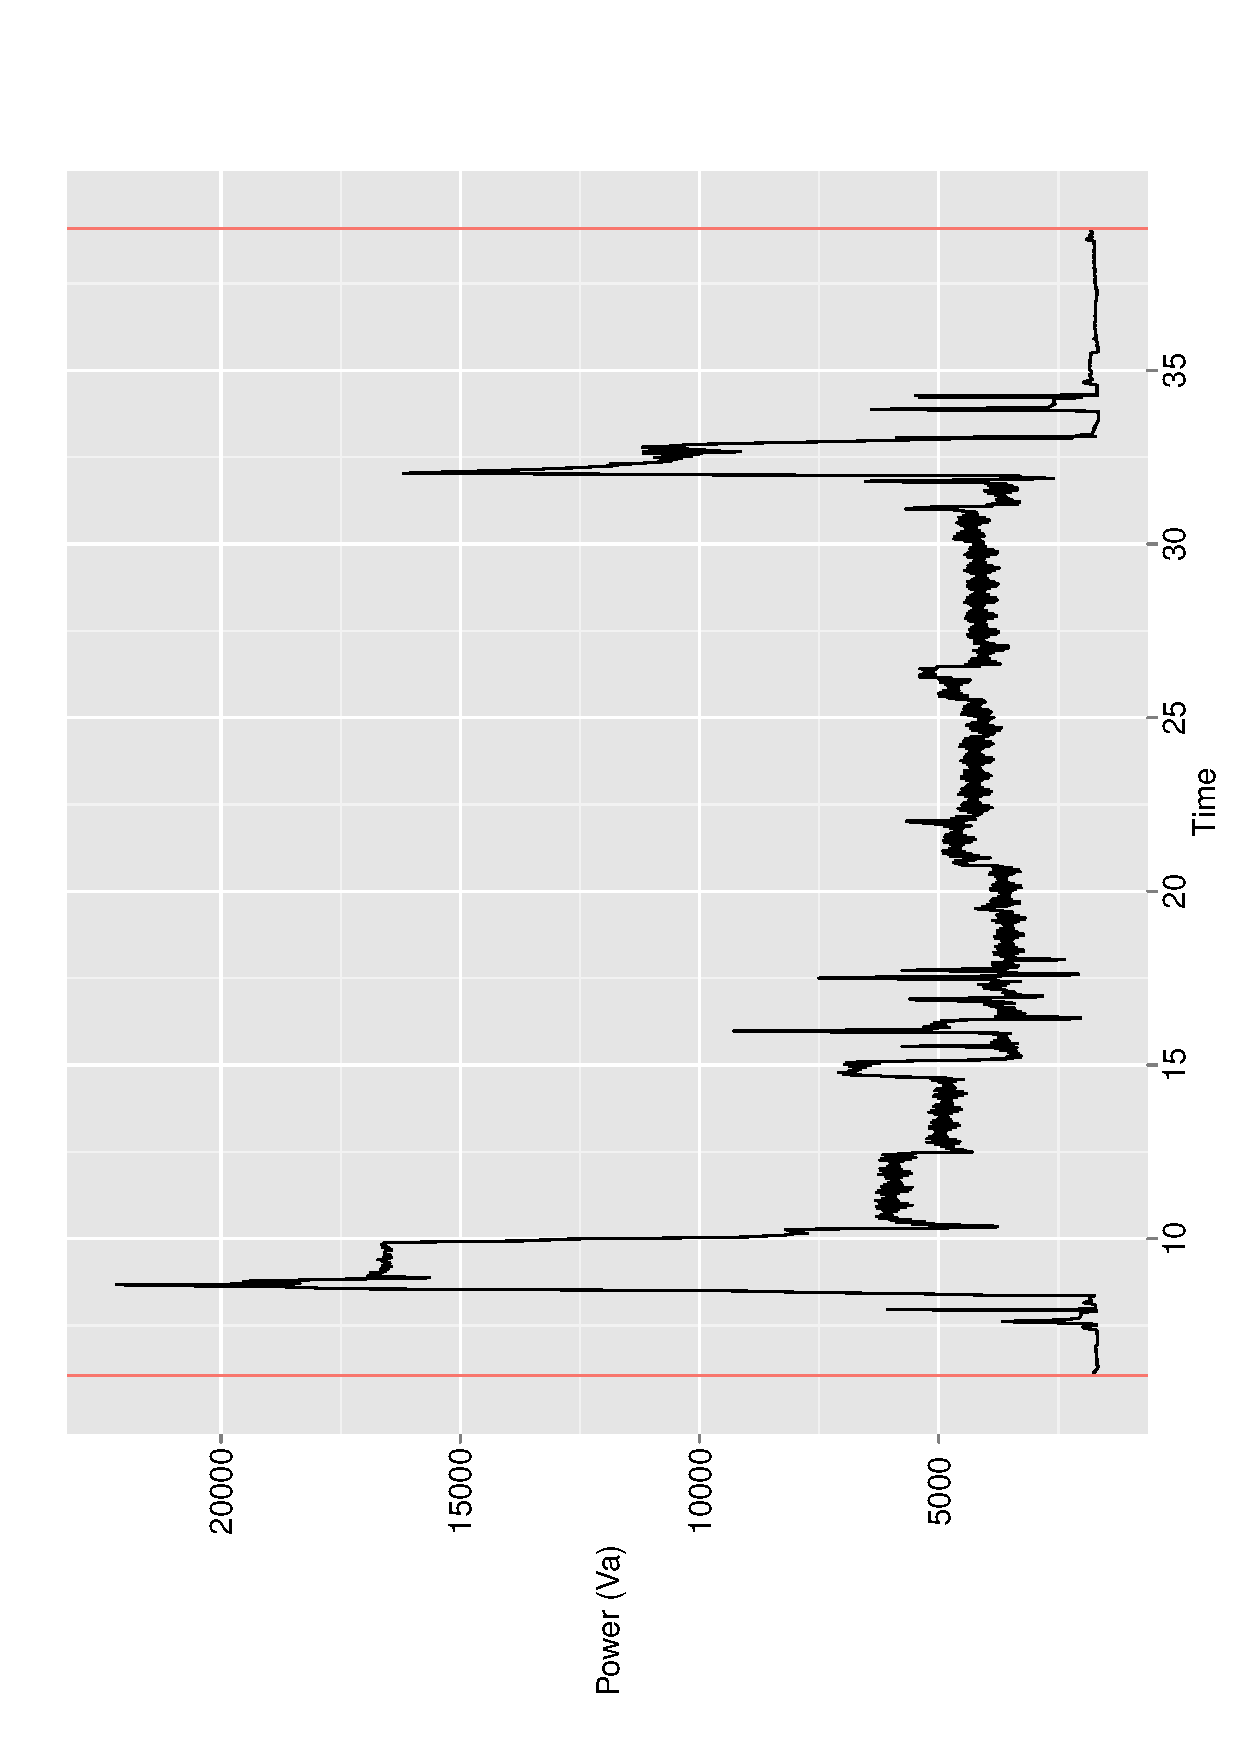
\includegraphics[width=14cm,height=8cm,keepaspectratio]{Images/uniform_split_1_section}\caption{Uniform split single section,\label{fig:Single-section-uniform}}
\end{figure}


The results have been summarised in Table \ref{tab:Single-section-uniform-ortho}
for orthonormal variables and in Table \ref{tab:Single-section-uniform-mixed}
for mixed polynomial variable.

\begin{table}
\noindent \begin{centering}
\begin{tabular}{|>{\centering}p{1.5cm}|>{\centering}p{1.5cm}|>{\centering}p{1.5cm}|>{\centering}p{1.5cm}|>{\centering}p{1.5cm}|>{\centering}p{1.5cm}|}
\hline 
Degree & Degree of Freedom & RMSE for test set ($\mu m$) & RMSE for training set($\mu m$) & Maximum error for test set($\mu m$) & Maximum error for training set($\mu m$)\tabularnewline
\hline 
\hline 
2 & 8 & 0.0990 & 0.0986 & 0.3566 & 0.3472\tabularnewline
\hline 
\hline 
3 & 12 & 0.0986 & 0.0983 & 0.3467 & 0.3430\tabularnewline
\hline 
\hline 
4 & 15 & 0.0997 & 0.0953 & 0.3002 & 0.3392\tabularnewline
\hline 
\hline 
5 & 19 & 0.0957 & 0.0929 & 0.2809 & 0.3437\tabularnewline
\hline 
\end{tabular}\caption{Single section uniform splitting, orthonormal polynomial variables\label{tab:Single-section-uniform-ortho}}

\par\end{centering}

\end{table}


\begin{table}
\noindent \centering{}%
\begin{tabular}{|>{\centering}p{1.5cm}|>{\centering}p{1.5cm}|>{\centering}p{1.5cm}|>{\centering}p{1.5cm}|>{\centering}p{1.5cm}|>{\centering}p{1.5cm}|}
\hline 
Degree & Degree of Freedom & RMSE for test set ($\mu m$) & RMSE for training set($\mu m$) & Maximum error for test set($\mu m$) & Maximum error for training set($\mu m$)\tabularnewline
\hline 
\hline 
2 & 8 & 0.0975 & 0.1007 & 0.3416 & 0.3480\tabularnewline
\hline 
\hline 
3 & 6 & 0.0976 & 0.1005 & 0.3443 & 0.3472\tabularnewline
\hline 
\hline 
4 & 12 & 0.0976 & 0.1006 & 0.3441 & 0.3466\tabularnewline
\hline 
\hline 
5 & 13 & 0.0976 & 0.1004 & 0.3390 & 0.3464\tabularnewline
\hline 
\end{tabular}\caption{Single section uniform split, mixed polynomial variables.\label{tab:Single-section-uniform-mixed}}
\end{table}



\subsubsection{Two sections}

Here, the cycle is split into two sections. Thus the cycle without
splits would look like Fig \ref{fig:Uiform-split--Two}.

\begin{figure}
\noindent \begin{centering}
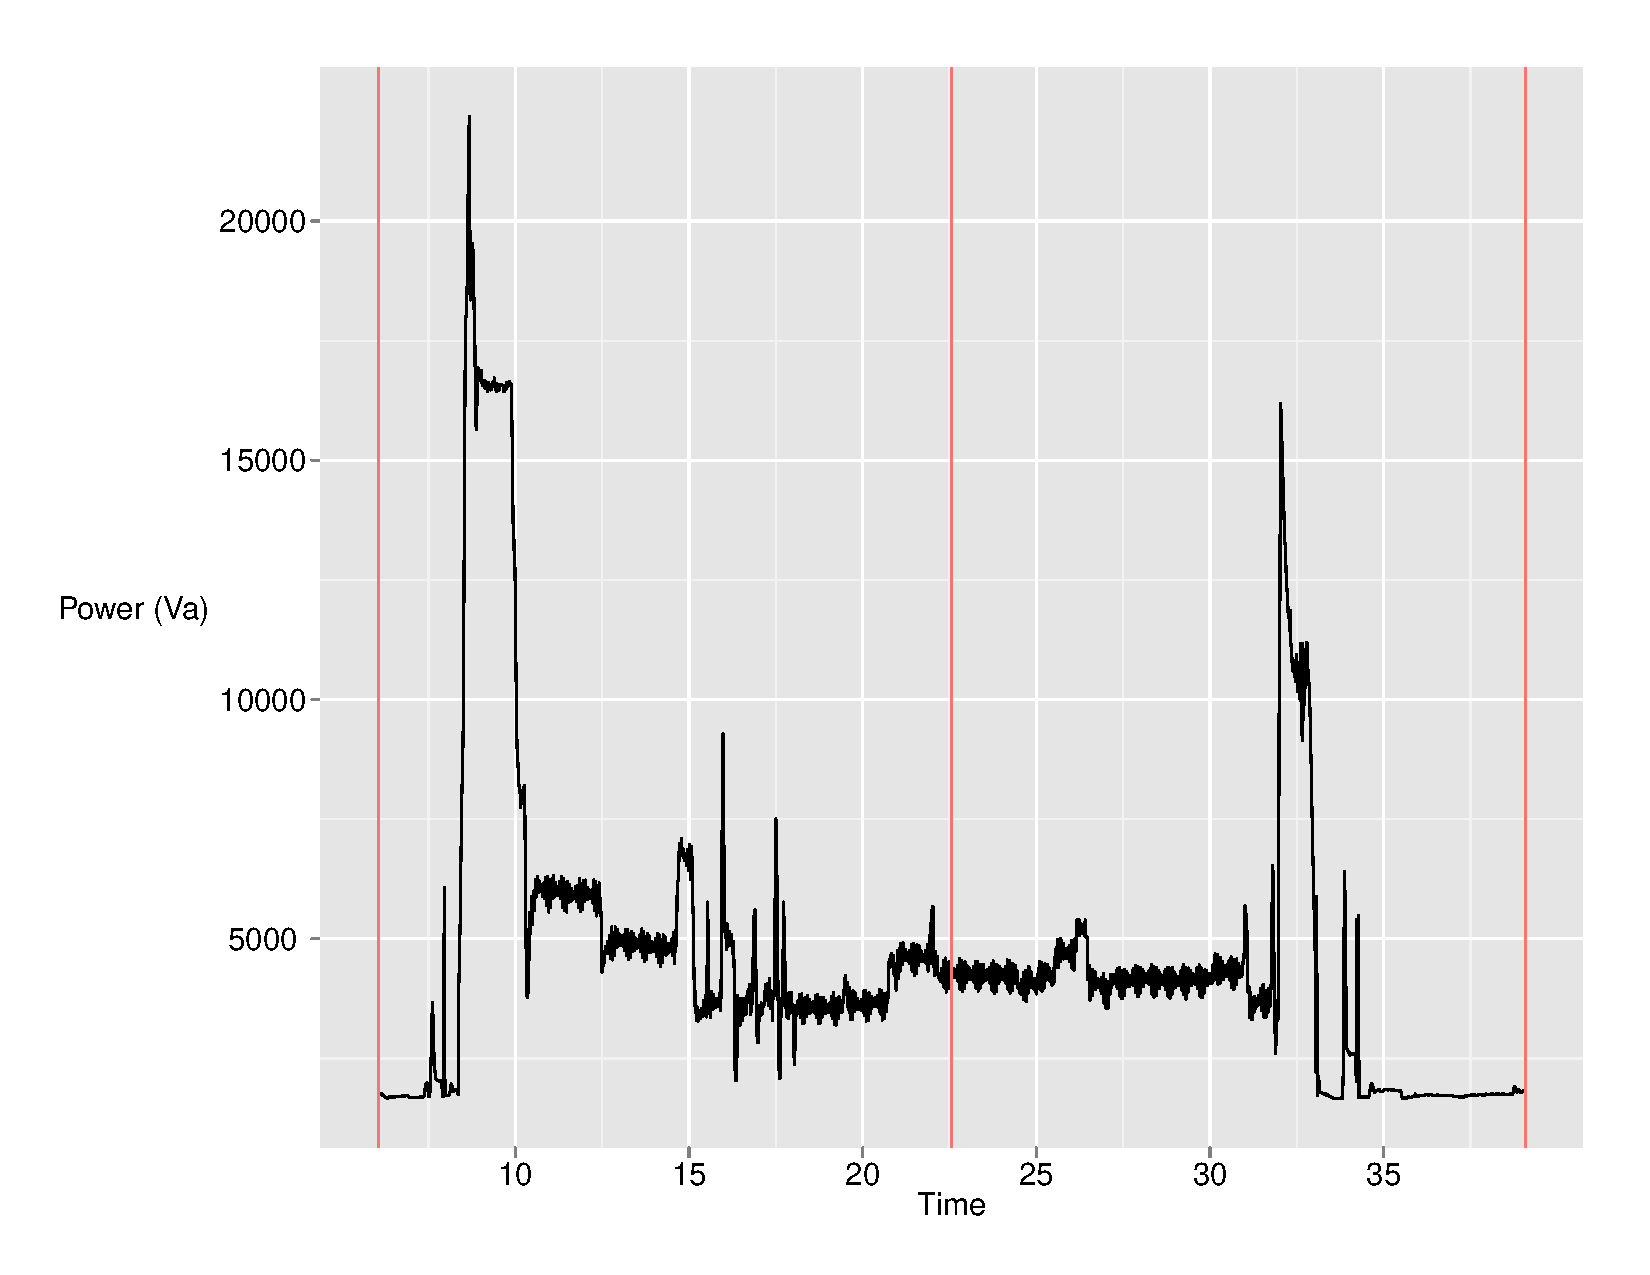
\includegraphics[width=14cm,height=8cm]{Images/uniform_split_2_section}\caption{Uiform split- Two sections\label{fig:Uiform-split--Two}}

\par\end{centering}

\end{figure}


The results have been summarised in Table \ref{tab:Uniform-splitting-2-section-ortho}
for orthonormal variables and in Table \ref{tab:Uniform-splitting-two-sections-mixed}
for mixed polynomial variable.

\begin{table}
\noindent \begin{centering}
\begin{tabular}{|>{\centering}p{1.5cm}|>{\centering}p{1.5cm}|>{\centering}p{1.5cm}|>{\centering}p{1.5cm}|>{\centering}p{1.5cm}|>{\centering}p{1.5cm}|}
\hline 
Degree & Degree of Freedom & RMSE for test set ($\mu m$) & RMSE for training set($\mu m$) & Maximum error for test set($\mu m$) & Maximum error for training set($\mu m$)\tabularnewline
\hline 
\hline 
2 & 8 & 0.0668 & 0.0586 & 0.4173 & 0.1650\tabularnewline
\hline 
\hline 
3 & 12 & 0.0645 & 0.0564 & 0.4235 & 0.1685\tabularnewline
\hline 
\hline 
4 & 15 & 0.0674 & 0.0564 & 0.4358 & 0.1777\tabularnewline
\hline 
\hline 
5 & 18 & 0.0685 & 0.0551 & 0.4072 & 0.1686\tabularnewline
\hline 
\end{tabular}\caption{Uniform splitting-two sections, orthonormal variables\label{tab:Uniform-splitting-2-section-ortho}}

\par\end{centering}

\end{table}


\begin{table}
\noindent \begin{centering}
\begin{tabular}{|>{\centering}p{1.5cm}|>{\centering}p{1.5cm}|>{\centering}p{1.5cm}|>{\centering}p{1.5cm}|>{\centering}p{1.5cm}|>{\centering}p{1.5cm}|}
\hline 
Degree & Degree of Freedom & RMSE for test set ($\mu m$) & RMSE for training set($\mu m$) & Maximum error for test set($\mu m$) & Maximum error for training set($\mu m$)\tabularnewline
\hline 
\hline 
2 & 9 & 0.0696 & 0.0581 & 0.4444 & 0.1523\tabularnewline
\hline 
\hline 
3 & 9 & 0.0689 & 0.0580 & 0.4405 & 0.1534\tabularnewline
\hline 
\hline 
4 & 13 & 0.0683 & 0.0576 & 0.4382 & 0.1550\tabularnewline
\hline 
\hline 
5 & 13 & 0.0677 & 0.0579 & 0.4287 & 0.1572\tabularnewline
\hline 
\end{tabular}\caption{Uniform splitting-two sections, mixed polynomial variables\label{tab:Uniform-splitting-two-sections-mixed}}

\par\end{centering}

\end{table}



\subsubsection{Three sections}

Here, the cycle is split into three sections. Thus the cycle without
splits would look like Fig \ref{fig:Uniform-split,-Three} and the
results have been summarised in Table \ref{tab:Uniform-splitting3-section-ortho}
for orthonormal polynomial variable and Table \ref{tab:Uniform-splitting-3-section-mixed}
for mixed polynomial variable.

\begin{figure}
\noindent \begin{centering}
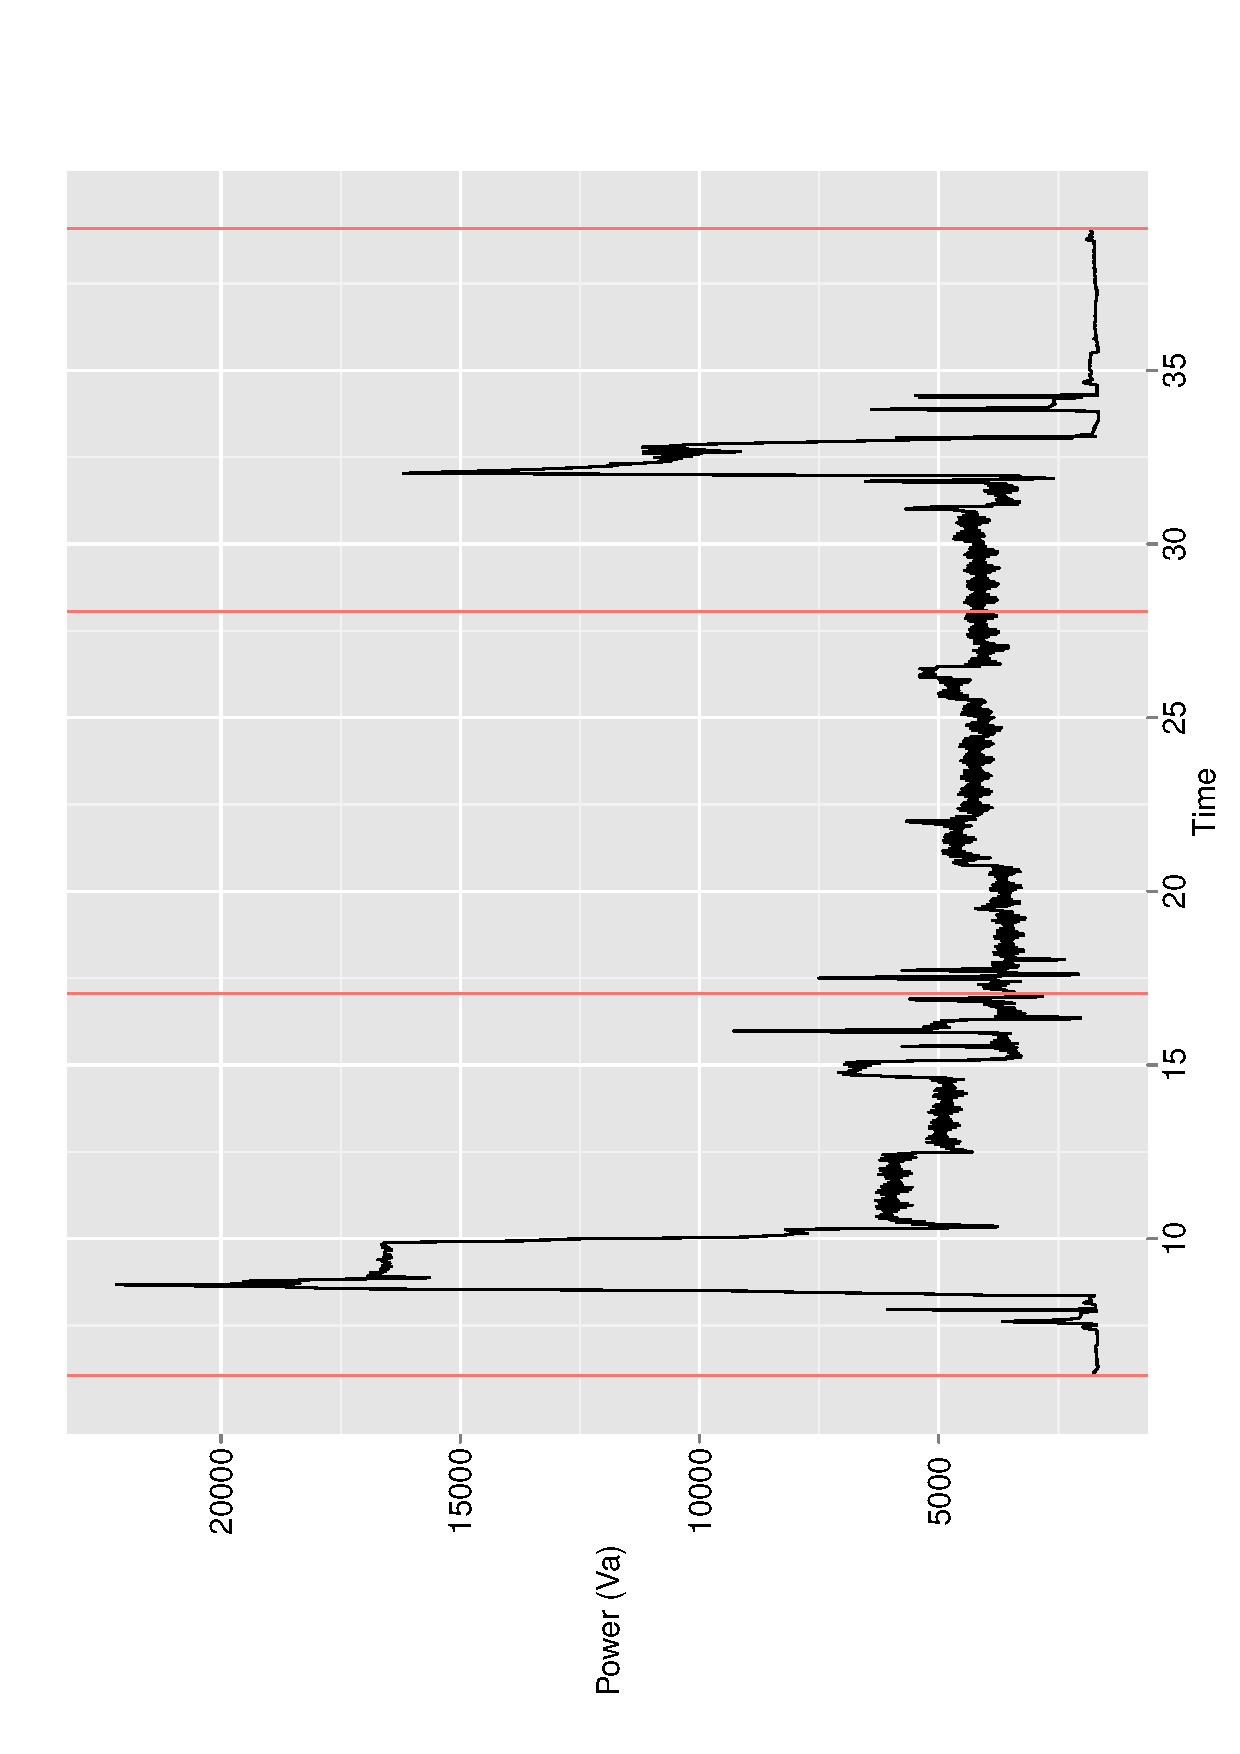
\includegraphics[width=14cm,height=8cm]{Images/uniform_split_3_section}\caption{Uniform split, Three sections\label{fig:Uniform-split,-Three}}

\par\end{centering}

\end{figure}


\begin{table}
\noindent \begin{centering}
\begin{tabular}{|>{\centering}p{1.5cm}|>{\centering}p{1.5cm}|>{\centering}p{1.5cm}|>{\centering}p{1.5cm}|>{\centering}p{1.5cm}|>{\centering}p{1.5cm}|}
\hline 
Degree & Degree of Freedom & RMSE for test set ($\mu m$) & RMSE for training set($\mu m$) & Maximum error for test set($\mu m$) & Maximum error for training set($\mu m$)\tabularnewline
\hline 
\hline 
2 & 12 & 0.0448 & 0.0413 & 0.1421 & 0.1679\tabularnewline
\hline 
\hline 
3 & 13 & 0.0480 & 0.0405 & 0.1483 & 0.1436\tabularnewline
\hline 
\hline 
4 & 13 & 0.0495 & 0.0416 & 0.1407 & 0.1336\tabularnewline
\hline 
\hline 
5 & 20 & 0.0522 & 0.0354 & 0.2816 & 0.1209\tabularnewline
\hline 
\end{tabular}\caption{Uniform splitting-three sections, orthonormal variables\label{tab:Uniform-splitting3-section-ortho}}

\par\end{centering}

\end{table}


\begin{table}
\noindent \begin{centering}
\begin{tabular}{|>{\centering}p{1.5cm}|>{\centering}p{1.5cm}|>{\centering}p{1.5cm}|>{\centering}p{1.5cm}|>{\centering}p{1.5cm}|>{\centering}p{1.5cm}|}
\hline 
Degree & Degree of Freedom & RMSE for test set ($\mu m$) & RMSE for training set($\mu m$) & Maximum error for test set($\mu m$) & Maximum error for training set($\mu m$)\tabularnewline
\hline 
\hline 
2 & 14 & 0.0431 & 0.0426 & 0.1399 & 0.2375\tabularnewline
\hline 
\hline 
3 & 9 & 0.0427 & 0.0454 & 0.1423 & 0.2728\tabularnewline
\hline 
\hline 
4 & 7 & 0.0427 & 0.0477 & 0.1417 & 0.2746\tabularnewline
\hline 
\hline 
5 & 9 & 0.0420 & 0.0466 & 0.1303 & 0.2706\tabularnewline
\hline 
\end{tabular}\caption{Uniform splitting-three sections, orthonormal variables\label{tab:Uniform-splitting-3-section-mixed}}

\par\end{centering}

\end{table}



\subsubsection{Five sections}

Here, the cycle is split into five sections. Thus the cycle without
splits would look like Fig \ref{fig:Uniform-splitting-Five-sections}
and the results have been summarised in Table \ref{tab:Uniform-splits,-Five-ortho}
for orthonormal variables and Table \ref{tab:Uniform-splits,Five-sections-mix}
for mixed polynomial variable.

\begin{figure}
\noindent \begin{centering}
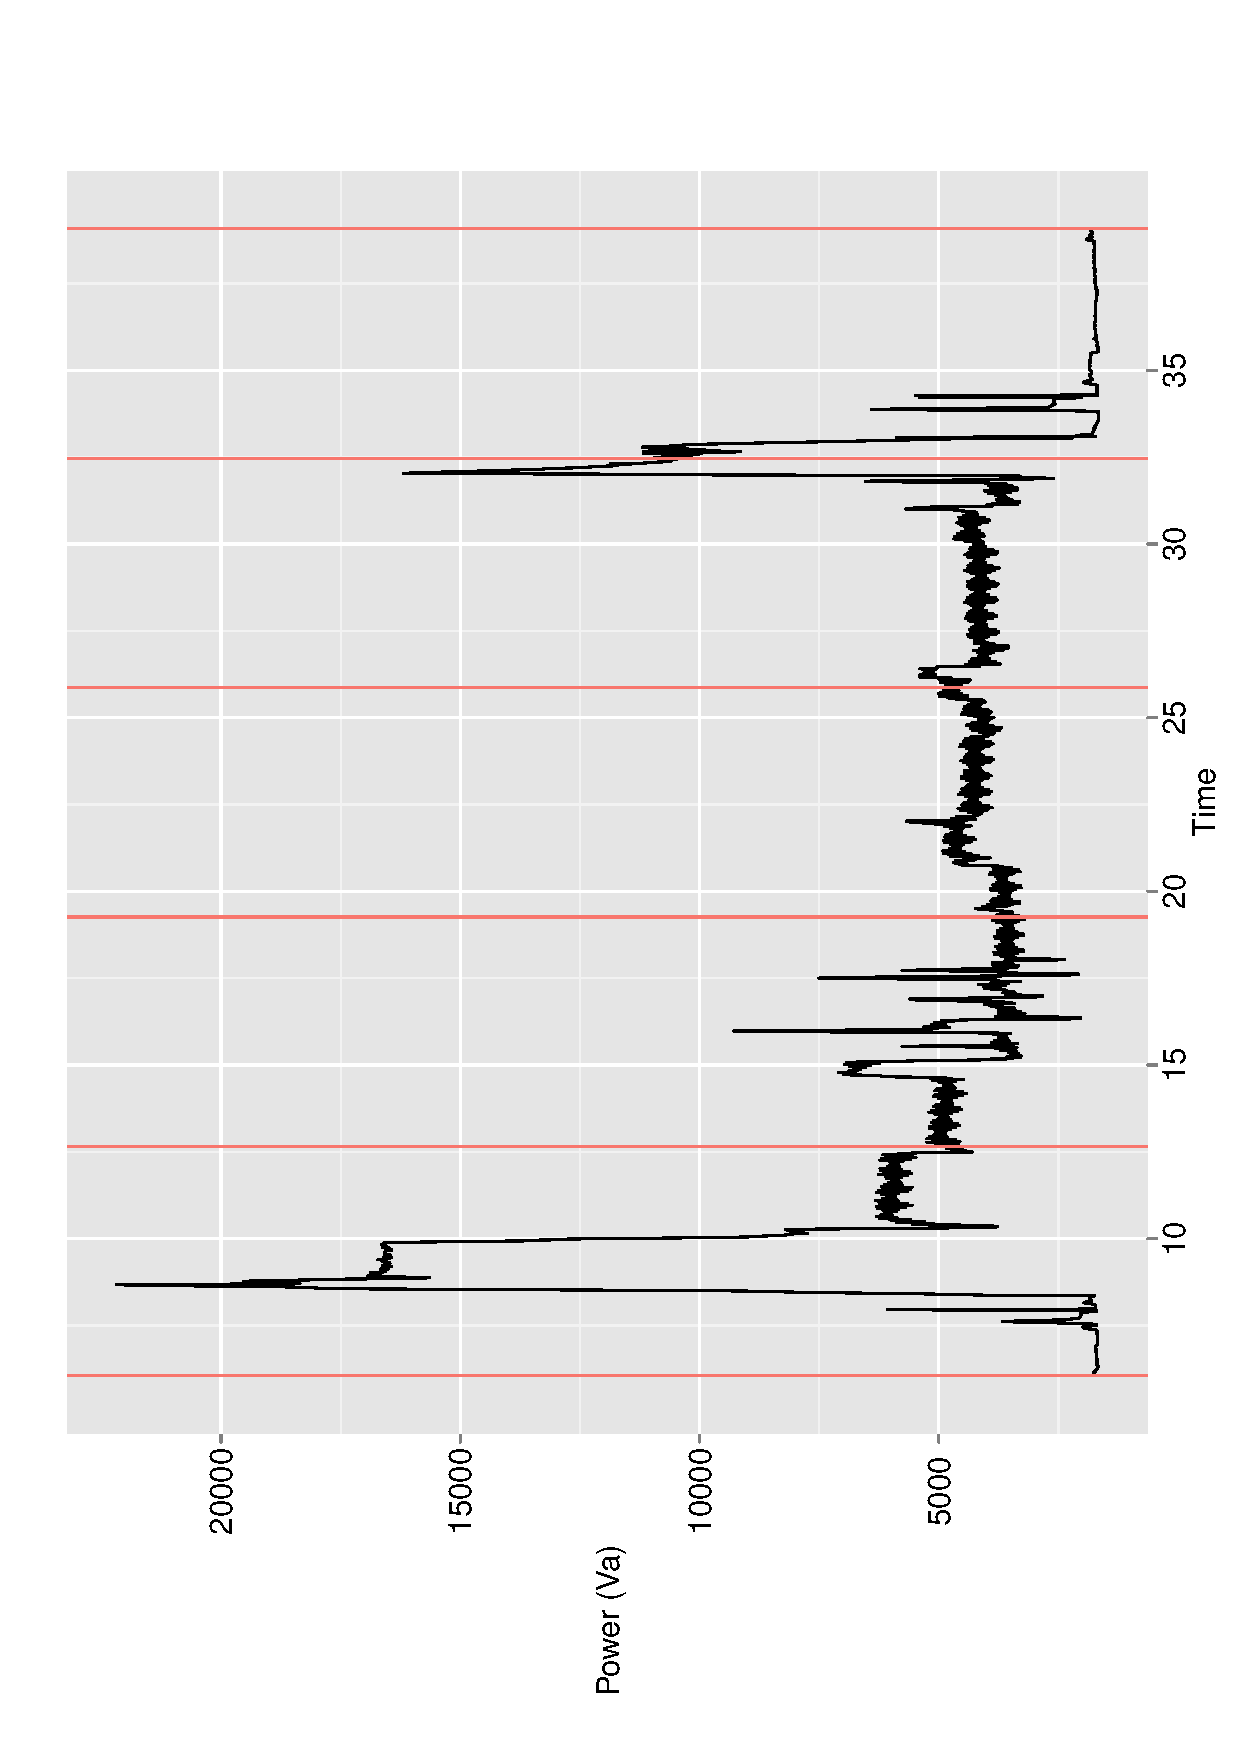
\includegraphics[width=14cm,height=8cm]{Images/uniform_split_5_section}\caption{Uniform splitting-Five sections \label{fig:Uniform-splitting-Five-sections}}

\par\end{centering}

\end{figure}


\begin{table}
\noindent \begin{centering}
\begin{tabular}{|>{\centering}p{1.5cm}|>{\centering}p{1.5cm}|>{\centering}p{1.5cm}|>{\centering}p{1.5cm}|>{\centering}p{1.5cm}|>{\centering}p{1.5cm}|}
\hline 
Degree & Degree of Freedom & RMSE for test set ($\mu m$) & RMSE for training set($\mu m$) & Maximum error for test set($\mu m$) & Maximum error for training set($\mu m$)\tabularnewline
\hline 
\hline 
2 & 20 & 0.0561 & 0.0285 & 0.4086 & 0.0835\tabularnewline
\hline 
\hline 
3 & 10 & 0.0647 & 0.0357 & 0.6190 & 0.1278\tabularnewline
\hline 
\hline 
4 & 10 & 0.0647 & 0.0357 & 0.6190 & 0.1278\tabularnewline
\hline 
\hline 
5 & 2 & 0.1156 & 0.0341 & 0.8198 & 0.2196\tabularnewline
\hline 
\end{tabular}\caption{Uniform splits, Five sections-Orthonormal variable polynomial \label{tab:Uniform-splits,-Five-ortho}}

\par\end{centering}

\end{table}


\begin{table}
\noindent \begin{centering}
\begin{tabular}{|>{\centering}p{1.5cm}|>{\centering}p{1.5cm}|>{\centering}p{1.5cm}|>{\centering}p{1.5cm}|>{\centering}p{1.5cm}|>{\centering}p{1.5cm}|}
\hline 
Degree & Degree of Freedom & RMSE for test set ($\mu m$) & RMSE for training set($\mu m$) & Maximum error for test set($\mu m$) & Maximum error for training set($\mu m$)\tabularnewline
\hline 
\hline 
2 & 11 & 0.0850 & 0.0315 & 0.8171 & 0.0984\tabularnewline
\hline 
\hline 
3 & 11 & 0.0881 & 0.0315 & 0.8564 & 0.0986\tabularnewline
\hline 
\hline 
4 & 14 & 0.0931 & 0.0316 & 0.9168 & 0.1009\tabularnewline
\hline 
\hline 
5 & 5 & 0.0977 & 0.0383 & 0.8786 & 0.1595\tabularnewline
\hline 
\end{tabular}\caption{Uniform splits,Five sections-mixed polynomial variable \label{tab:Uniform-splits,Five-sections-mix}}

\par\end{centering}

\end{table}



\subsubsection{Six sections}

Here, the cycle is split into six sections. Thus the cycle without
splits would look like Fig \ref{fig:Uniform-splitting-Six-sections}
and the results have been summarised in Table \ref{tab:Uniform-splits,Six-sections-Orth}
for orthonormal variables and Table \ref{tab:Uniform-splits,Six-sections-mix}
for mixed polynomial variable.

\begin{figure}
\noindent \begin{centering}
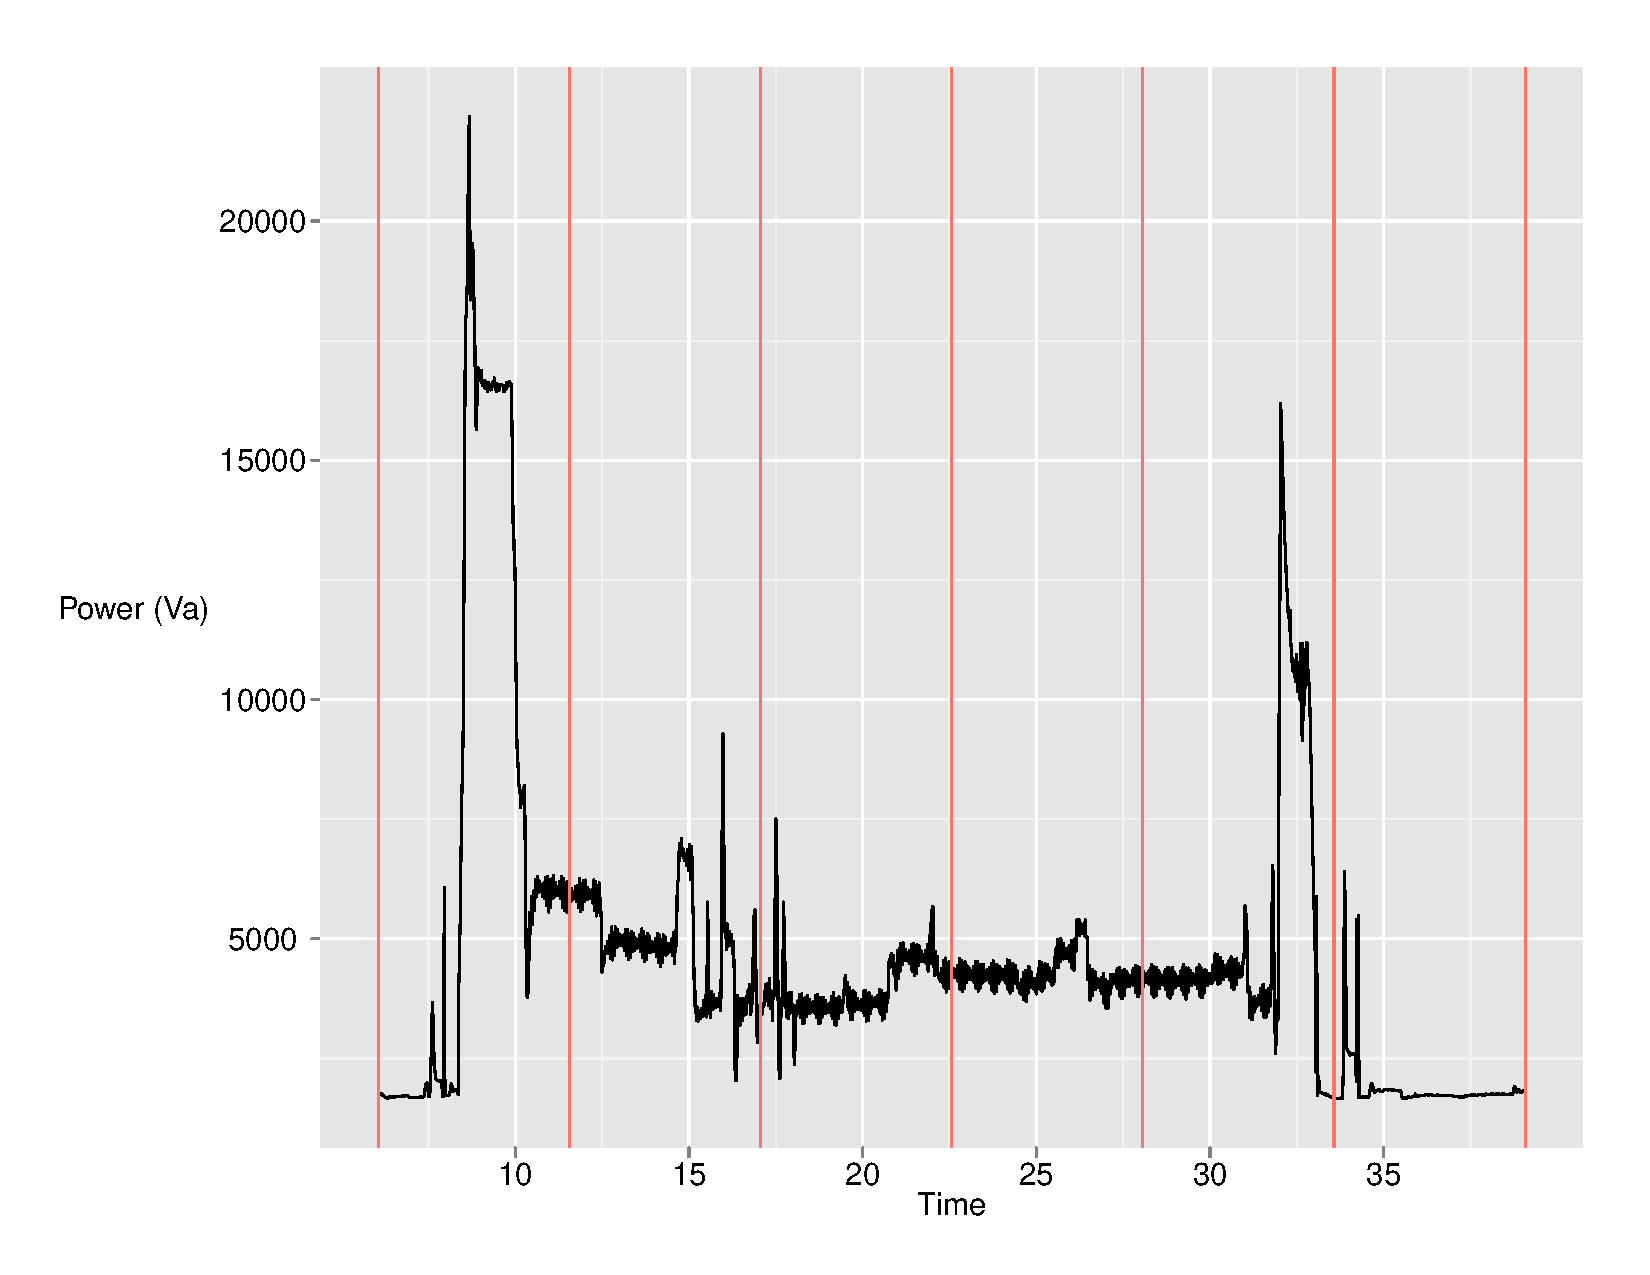
\includegraphics[width=14cm,height=8cm]{Images/uniform_split_6_section}\caption{Uniform splitting-Six sections \label{fig:Uniform-splitting-Six-sections}}

\par\end{centering}

\end{figure}


\begin{table}
\noindent \begin{centering}
\begin{tabular}{|>{\centering}p{1.5cm}|>{\centering}p{1.5cm}|>{\centering}p{1.5cm}|>{\centering}p{1.5cm}|>{\centering}p{1.5cm}|>{\centering}p{1.5cm}|}
\hline 
Degree & Degree of Freedom & RMSE for test set ($\mu m$) & RMSE for training set($\mu m$) & Maximum error for test set($\mu m$) & Maximum error for training set($\mu m$)\tabularnewline
\hline 
\hline 
2 & 23 & 0.0367 & 0.0226 & 0.2078 & 0.0797\tabularnewline
\hline 
\hline 
3 & 34 & 0.0409 & 0.0207 & 0.2424 & 0.0728\tabularnewline
\hline 
\hline 
4 & 44 & 0.0397 & 0.0200 & 0.2355 & 0.0750\tabularnewline
\hline 
\hline 
5 & 28 & 0.0502 & 0.0242 & 0.3099 & 0.0731\tabularnewline
\hline 
\end{tabular}\caption{Uniform splits,Six sections-Orthonormal variables \label{tab:Uniform-splits,Six-sections-Orth}}

\par\end{centering}

\end{table}


\begin{table}
\noindent \begin{centering}
\begin{tabular}{|>{\centering}p{1.5cm}|>{\centering}p{1.5cm}|>{\centering}p{1.5cm}|>{\centering}p{1.5cm}|>{\centering}p{1.5cm}|>{\centering}p{1.5cm}|}
\hline 
Degree & Degree of Freedom & RMSE for test set ($\mu m$) & RMSE for training set($\mu m$) & Maximum error for test set($\mu m$) & Maximum error for training set($\mu m$)\tabularnewline
\hline 
\hline 
2 & 75 & 0.0382 & 0.0215 & 0.1901 & 0.0855\tabularnewline
\hline 
\hline 
3 & 11 & 0.0395 & 0.0279 & 0.1959 & 0.0914\tabularnewline
\hline 
\hline 
4 & 13 & 0.0383 & 0.0265 & 0.1980 & 0.0902\tabularnewline
\hline 
\hline 
5 & 17 & 0.0373 & 0.0256 & 0.1973 & 0.0960\tabularnewline
\hline 
\end{tabular}\caption{Uniform splits,Six sections - mixed polynomial variable \label{tab:Uniform-splits,Six-sections-mix}}

\par\end{centering}

\end{table}



\subsubsection{\label{sub:Discussion-uniform splitting}Discussion}

Here we are primarily concerned with the RMSE value of each solution.
As we can see from the tables:-
\begin{enumerate}
\item Usually, the orthonormal and mixed polynomials offer outputs usually
have more or less similar values of RMSE. However, the time taken
to implement the 'mixed polynomial variable' method increases much
more rapidly than the 'orthonormal variables method' as we increase
the degree and number of splits.
\item For higher degree orthonormal variables' method, we may get high RMSE
due to usually just ONE extremely high error value which indicates
.
\item For most of the cases, the RMSE remains more or less the same as we
change the degree keeping other factors constant.
\item Usually, as we increase the number of splits, the RMSE value keeps
on dropping until we reach five sections where we see the RMSE shoot
up after which the RMSE goes back down. Although this may seem to
be an anomaly in the begining, there is a perfectly reasonable explanation
for which becomes evident when we have a look at the way the splits
are made. In all the splits, save for 5 splits, the significant spike
which occurs in the range of 30-35 seconds is untouched and the entire
feature falls into one section. However, this is not the case for
5 splits. The split midway the feature masks the contribution of the
pattern as a whole. This is not surprising as the quality parameter
we are measuring (Ra) would depend heavily on the finishing cut of
the tool which takes place near the end of the cycle.
\end{enumerate}

\subsection{Feedback Splitting}

As seen in \ref{sub:Cycle-splitting}, in this we first hypothesize
a split and run our algorithm to obtain a solution. If this solution
provides significant improvement, we retain the split and move on
to make further splits. We have two ways to make these succesive splits.
We could approach this splitting either from start of the cycle (\textbf{Forward
feedback splitting}) or the end of the cycle (\textbf{Reverse feedback
splitting}). Here we will show the various cases where we vary the
direction of splitting, the threshold of relative difference of error
and type of method used for variable creation (mixed polynomial or
orthogonal polynomial). The results will be shown as two graphs where
one will represent the splits in the cycle and the other the trend
in the RMSE. We will also be showing the final RMSE value that we
obtain using the method.


\subsubsection{Forward feeback splits-Mixed polynomial-5\% relative change of RMSE
threshold}

\begin{figure}
\noindent \centering{}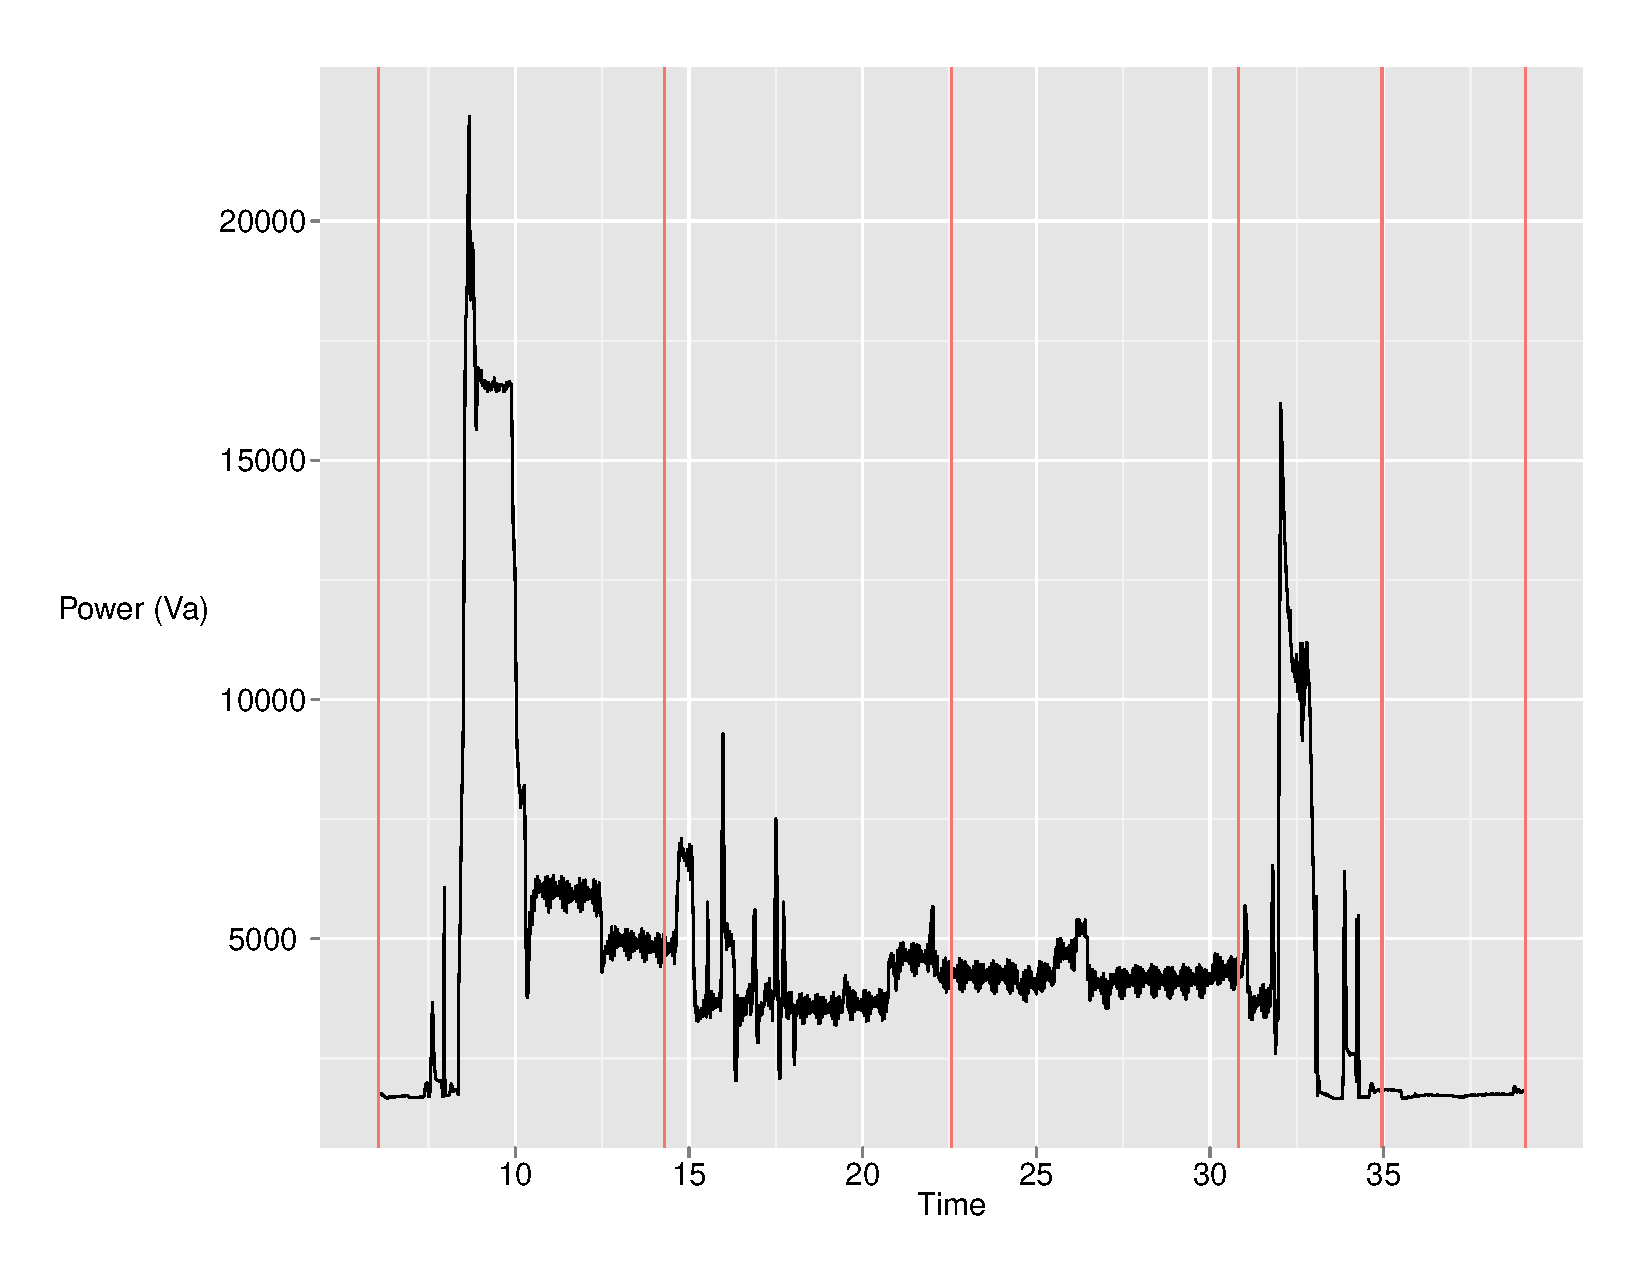
\includegraphics[width=14cm,height=8cm]{Images/5_per_fwd_mix_split}\caption{Mixed polynomial forward feedback splits with 5\% threshold for relative
change in RMSE- Cycle splits \label{fig:Mixed-polynomial-forward-5-splits}}
\end{figure}


\begin{figure}
\noindent \begin{centering}
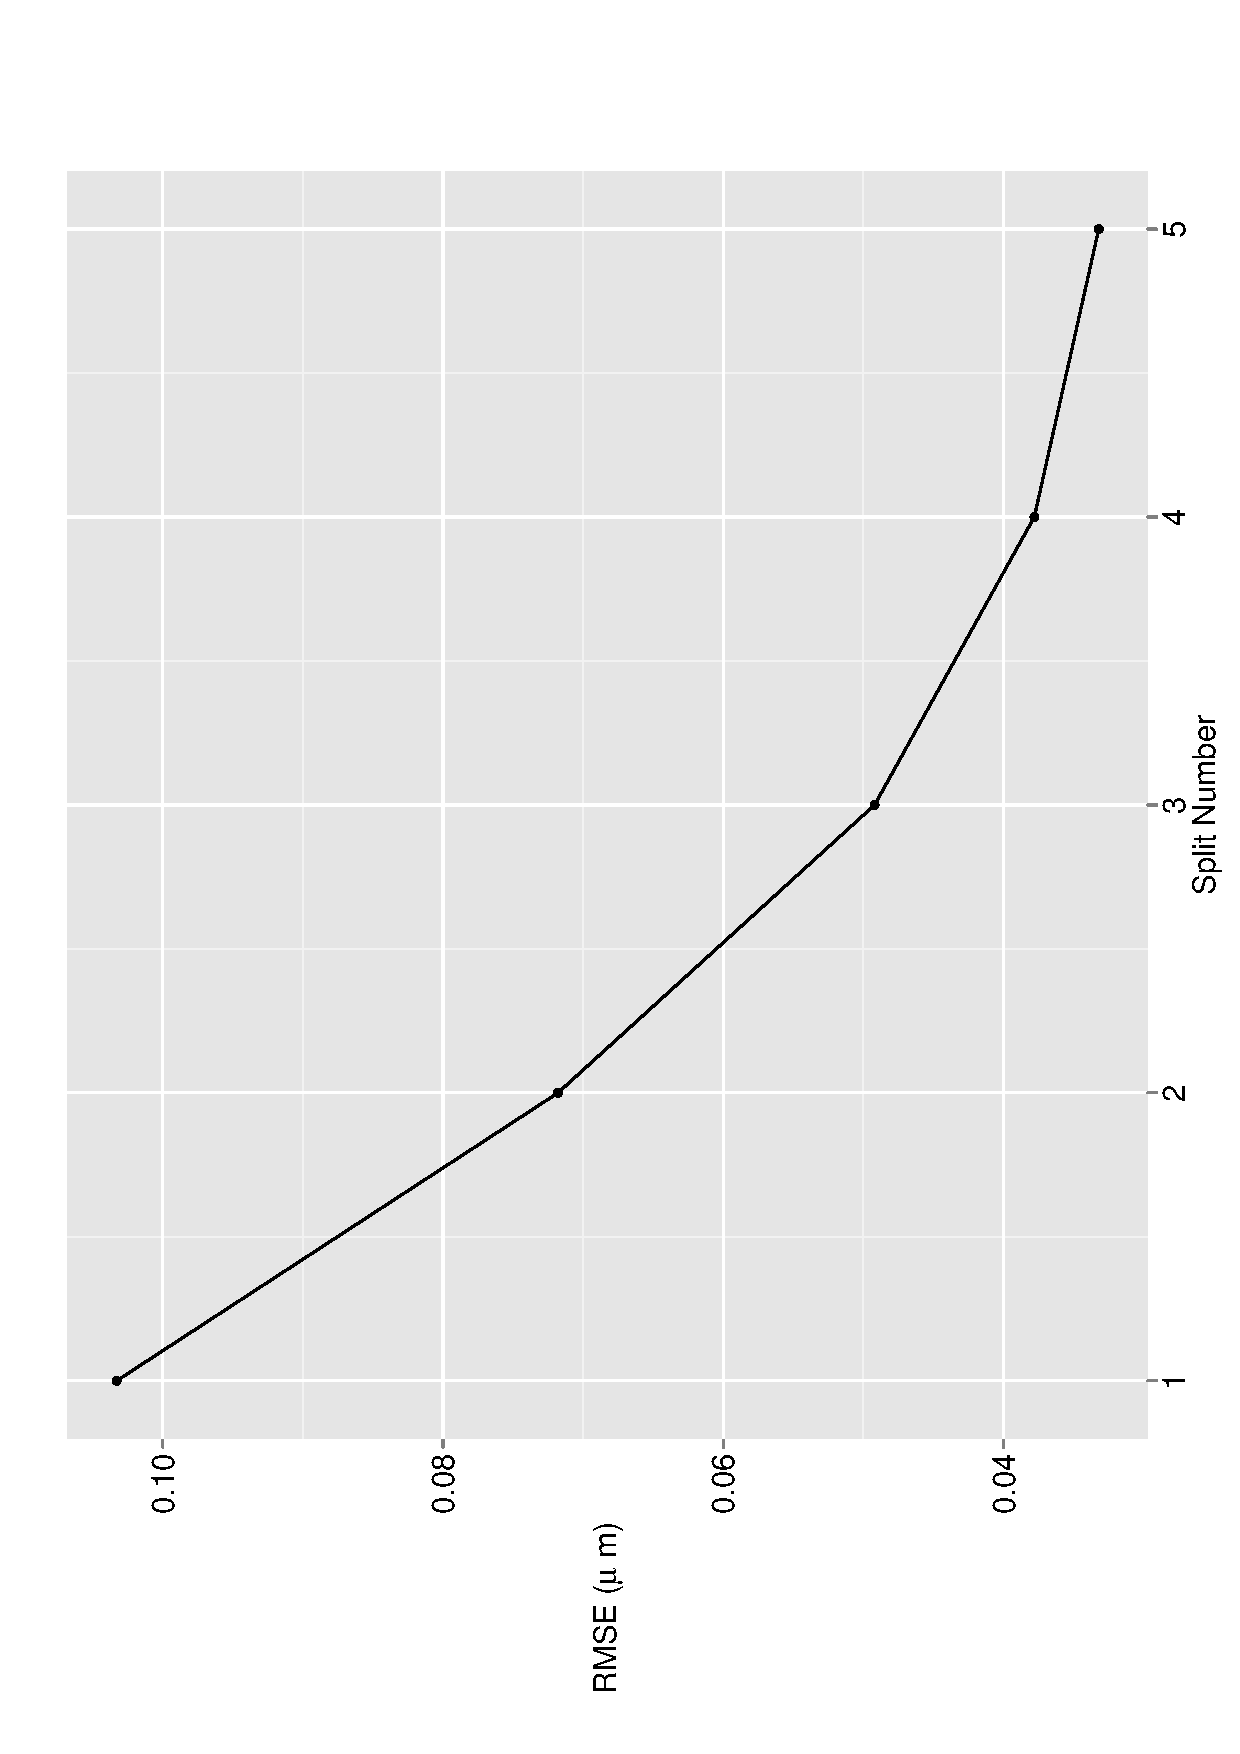
\includegraphics[width=14cm,height=8cm]{Images/5_per_fwd_mix_err}\caption{Mixed polynomial forward feedback splits with 5\% threshold for relative
change in RMSE- RMSE trends \label{fig:Mixed-polynomial-forward-5-err}}

\par\end{centering}

\end{figure}


The emergent splits are shown in Fig \ref{fig:Mixed-polynomial-forward-5-splits}
and the RMSE trend can be seen in Fig \ref{fig:Mixed-polynomial-forward-5-err}.
The final RMSE value was $0.0332\mu m$.


\subsubsection{Forward feedback splits- Orthonormal variables-5\% relative change
of RMSE threshold}

\begin{figure}
\noindent \begin{centering}
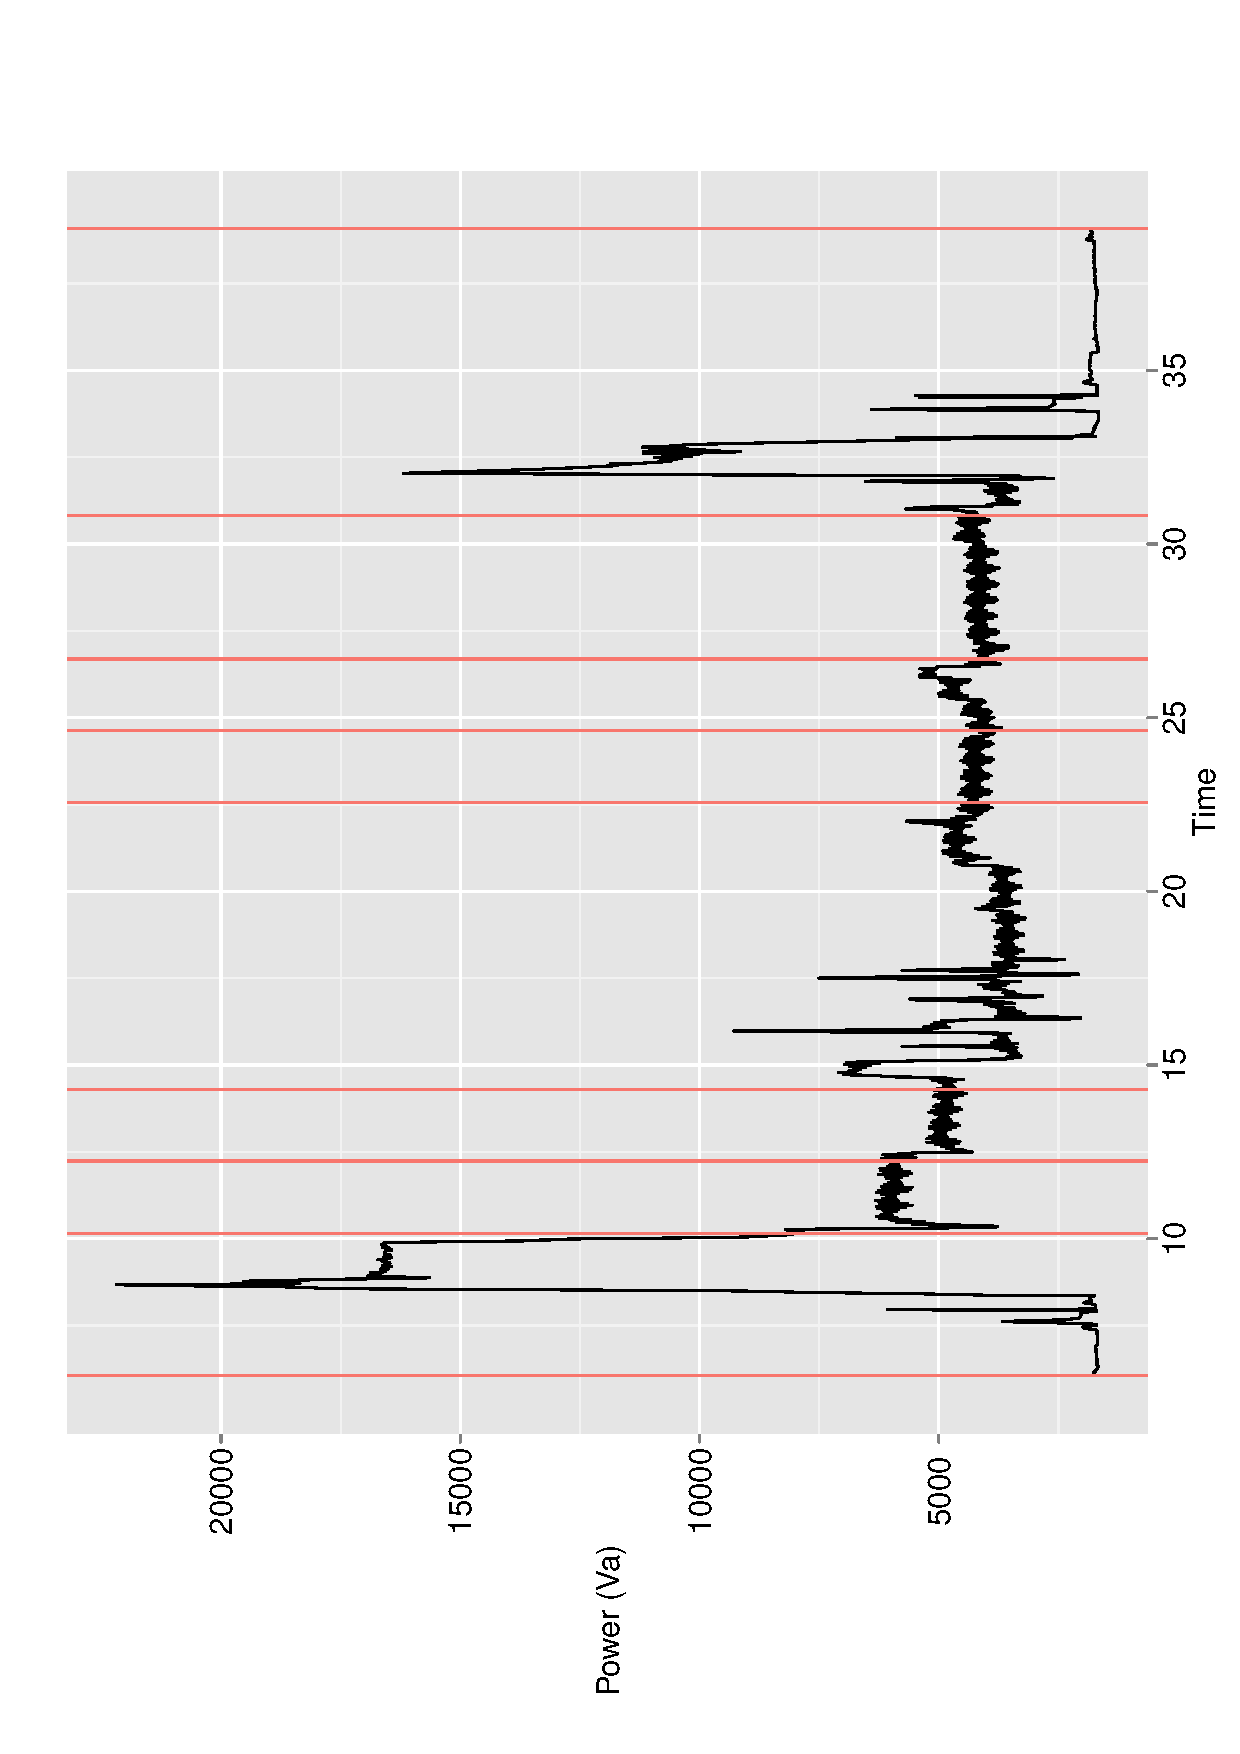
\includegraphics[width=14cm,height=8cm]{Images/1_per_frwd_ortho_split}\caption{Forward feedback splits-Orthonormal variables-5\% relative change
of RMSE threshold -Cycle splits \label{fig:Forward-feedback-splits-Orthonor-5-split}}

\par\end{centering}

\end{figure}


\begin{figure}
\noindent \begin{centering}
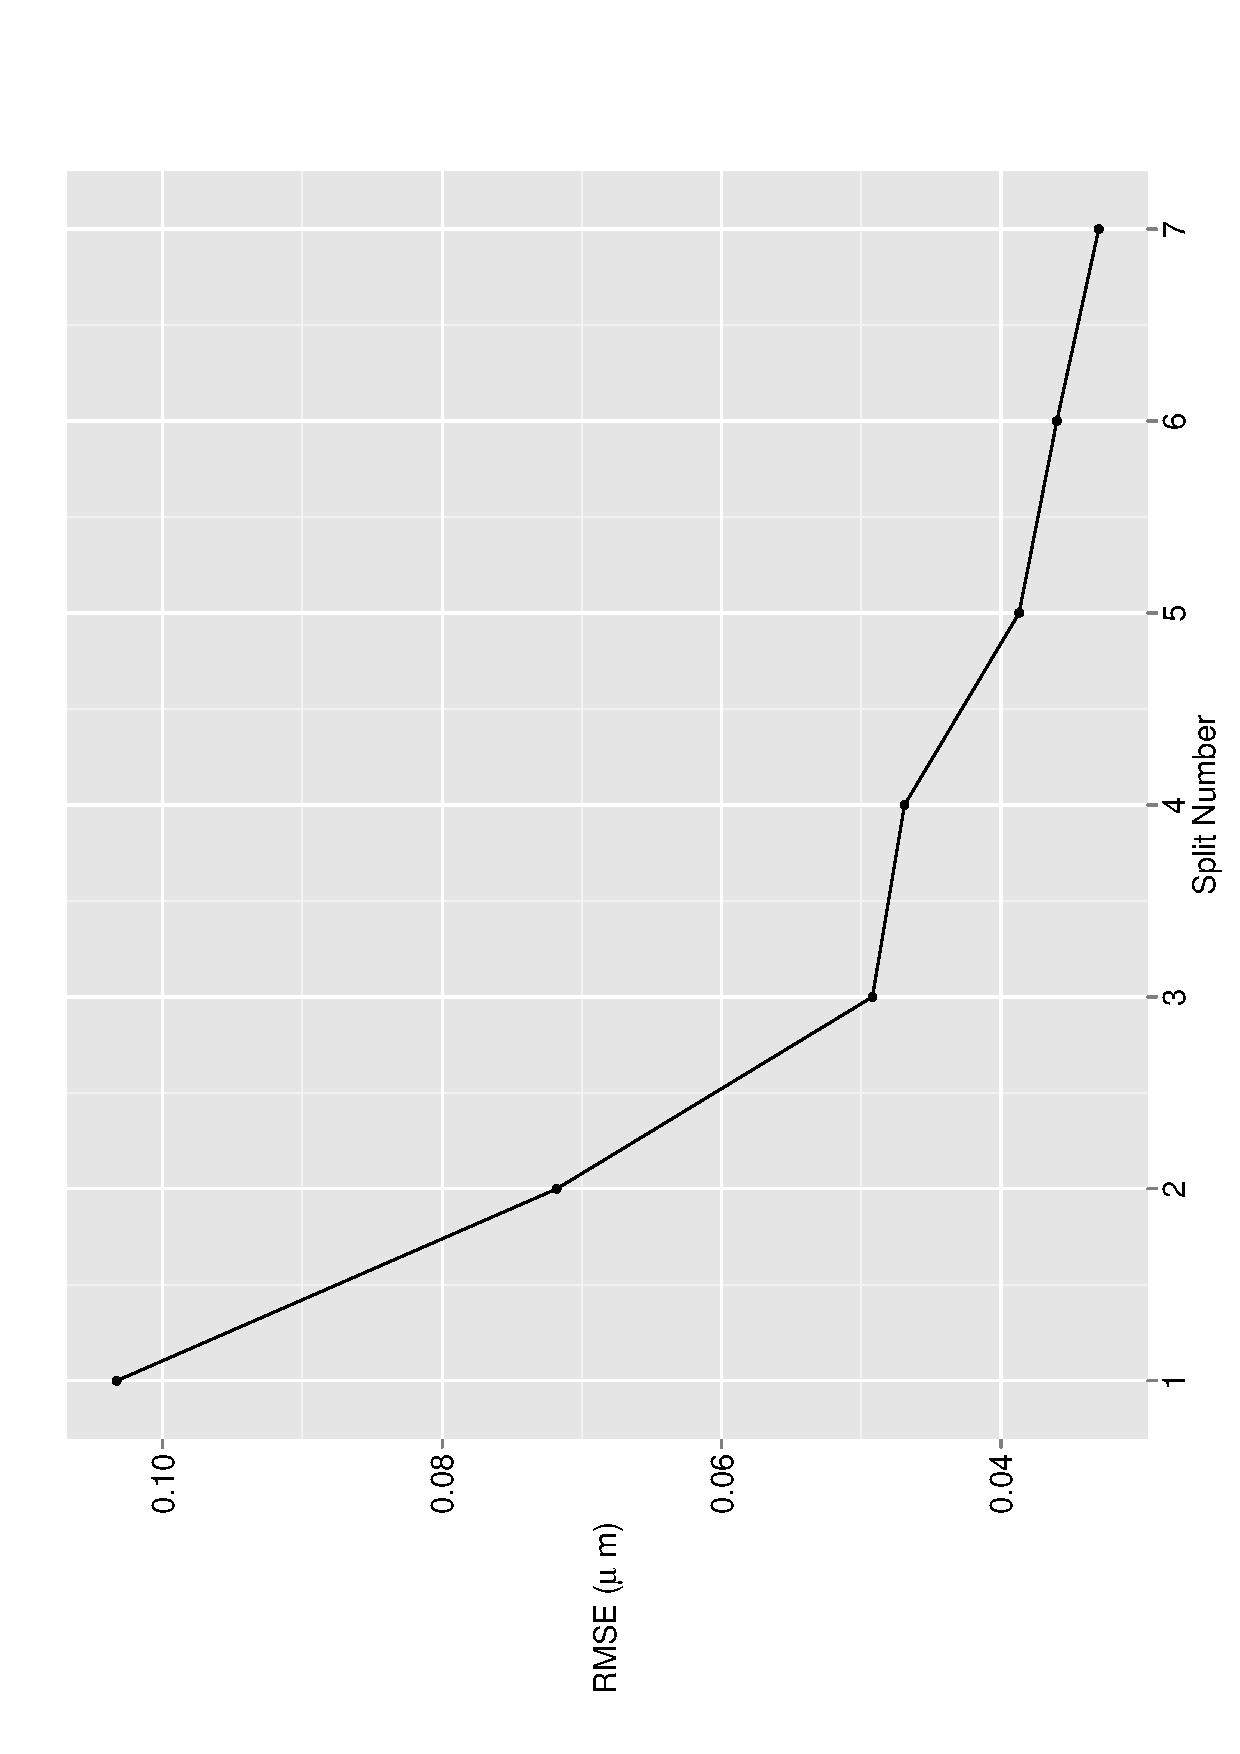
\includegraphics[width=14cm,height=8cm]{Images/1_per_frwd_mix_err}\caption{Forward feedback splits-Orthonormal variables-5\% relative change
of RMSE threshold - RMSE trend \label{fig:Forward-feedback-splits-Orthonor-5-err}}

\par\end{centering}

\end{figure}


The emergent splits are shown in Fig \ref{fig:Forward-feedback-splits-Orthonor-5-split}
and the RMSE trend can be seen in Fig \ref{fig:Forward-feedback-splits-Orthonor-5-err}.
The final RMSE value is $0.0365\mu m$.


\subsubsection{Forward feedback splits- Mixed polynomial-1\% relative change of
RMSE threshold}

\begin{figure}
\noindent \begin{centering}
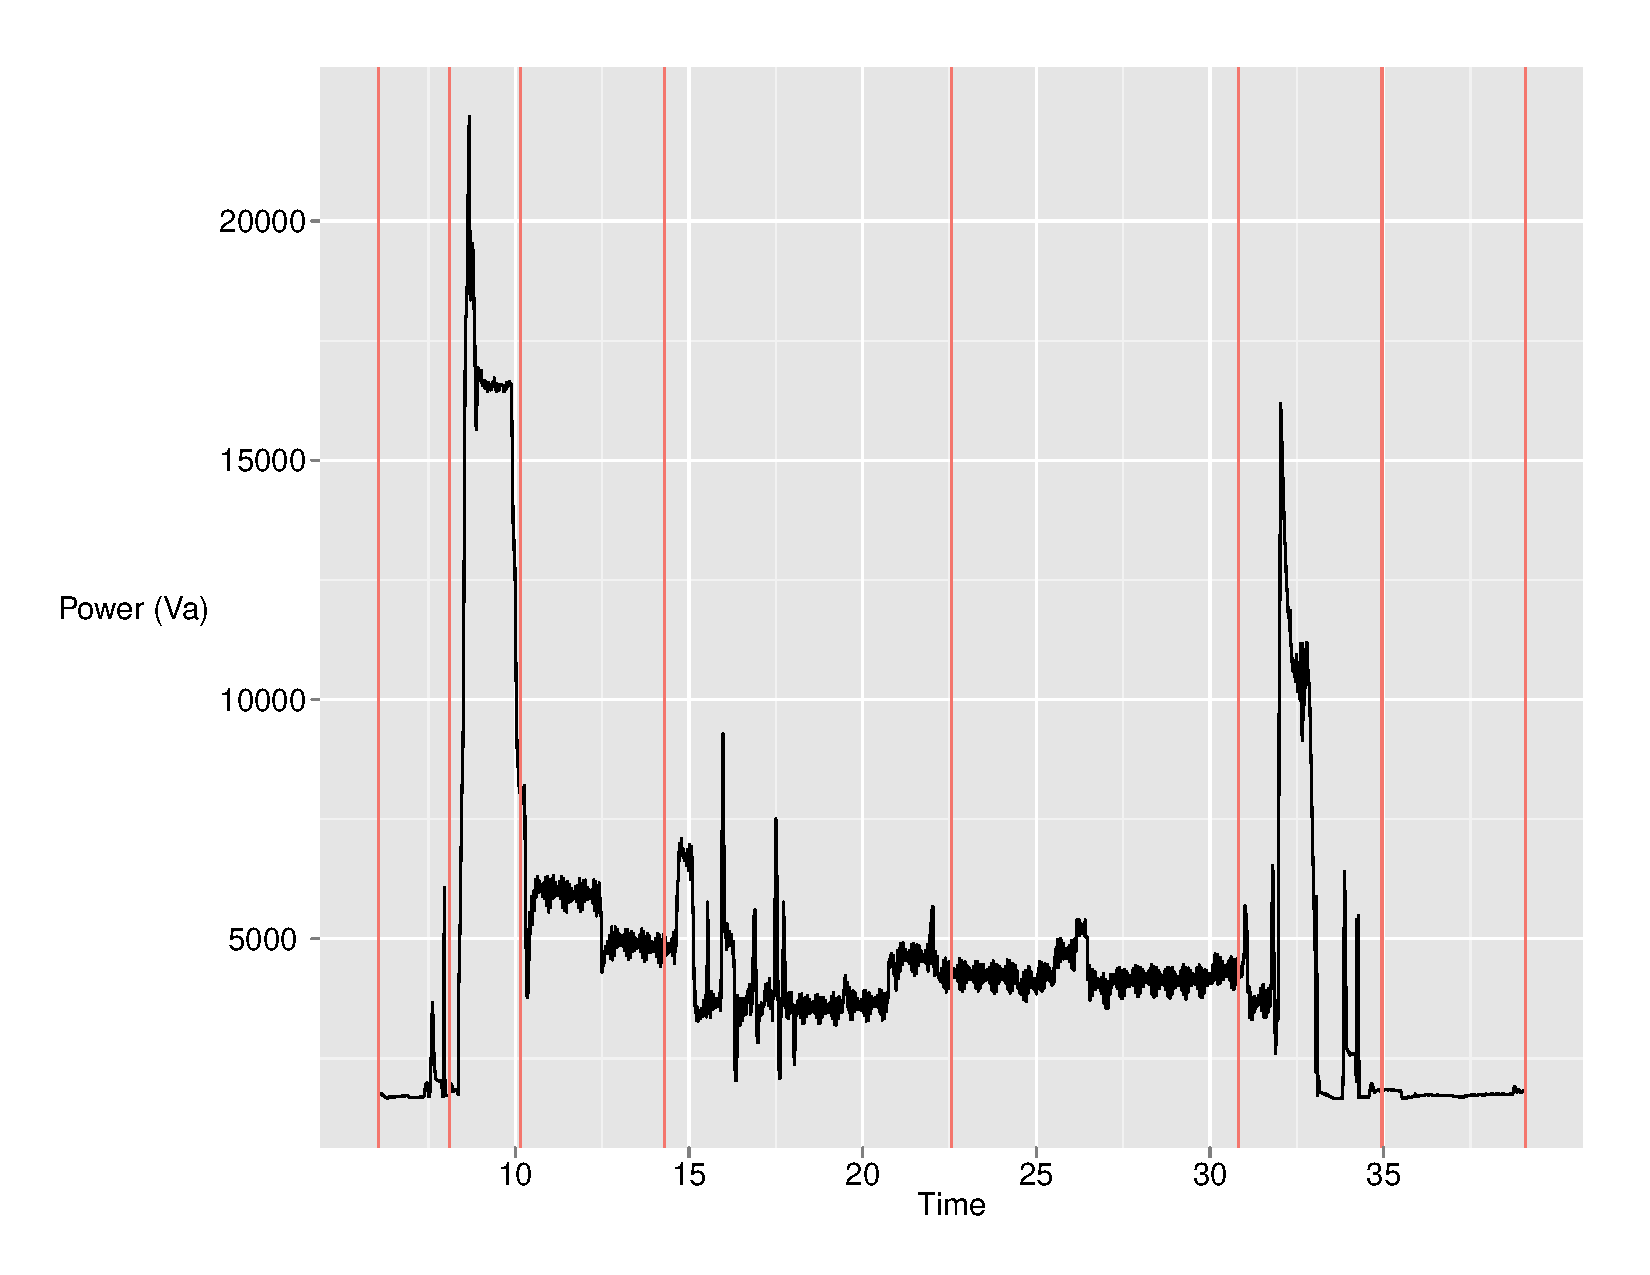
\includegraphics[width=14cm,height=8cm]{Images/1_per_frwd_mix_split}\caption{Mixed polynomial forward feedback splits with 1\% threshold for relative
change in RMSE- Cycle splits \label{fig:Mixed-polynomial-forward-1-split}}

\par\end{centering}

\end{figure}


\begin{figure}
\noindent \begin{centering}
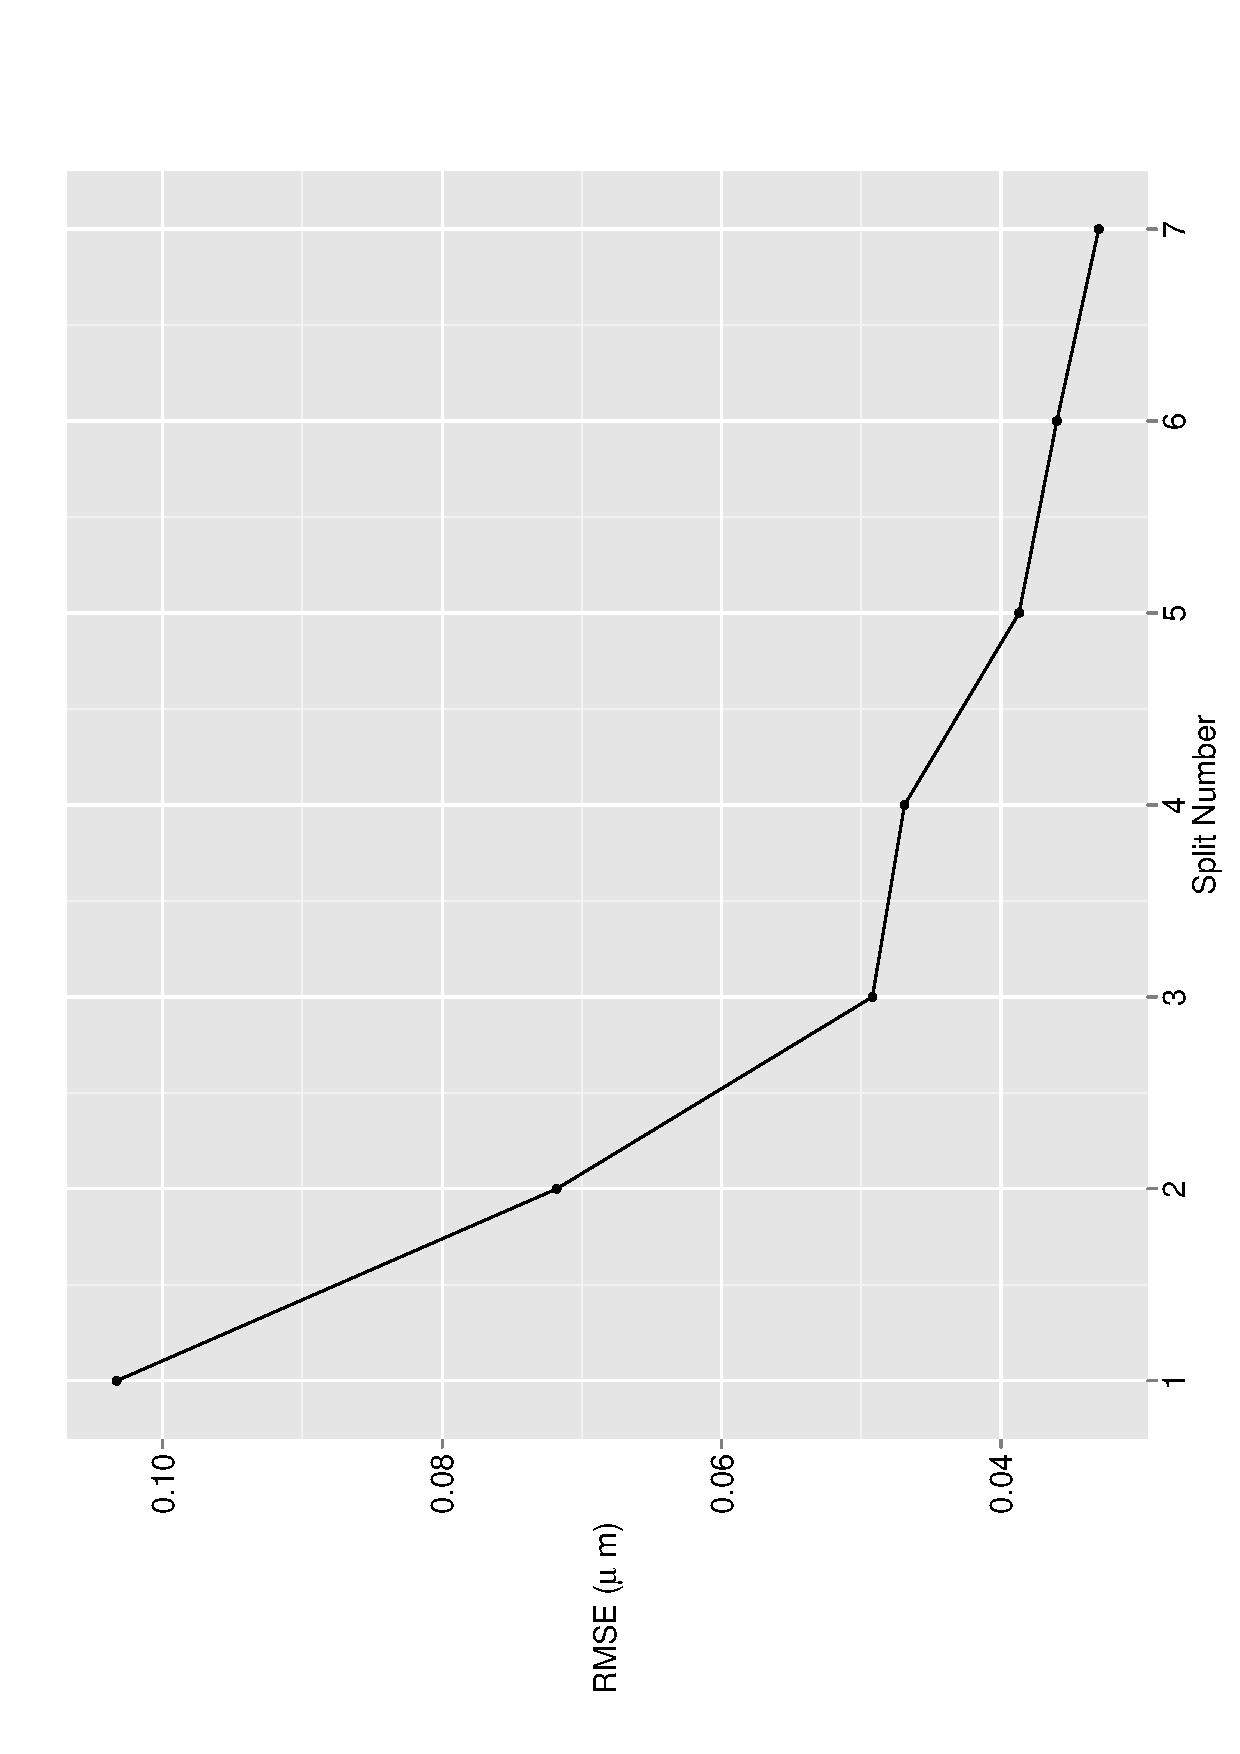
\includegraphics[width=14cm,height=8cm]{Images/1_per_frwd_mix_err}\caption{Mixed polynomial forward feedback splits with 1\% threshold for relative
change in RMSE- RMSE trend \label{fig:Mixed-polynomial-forward-1-err}}

\par\end{centering}

\end{figure}


The emergent splits are shown in Fig \ref{fig:Mixed-polynomial-forward-1-split}
and the RMSE trend can be seen in Fig \ref{fig:Mixed-polynomial-forward-1-err}.
The final RMSE value is $0.0330\mu m$.


\subsubsection{Forward feedback splits- Orthonormal variables-1\% relative change
of RMSE threshold}

\begin{figure}
\noindent \begin{centering}
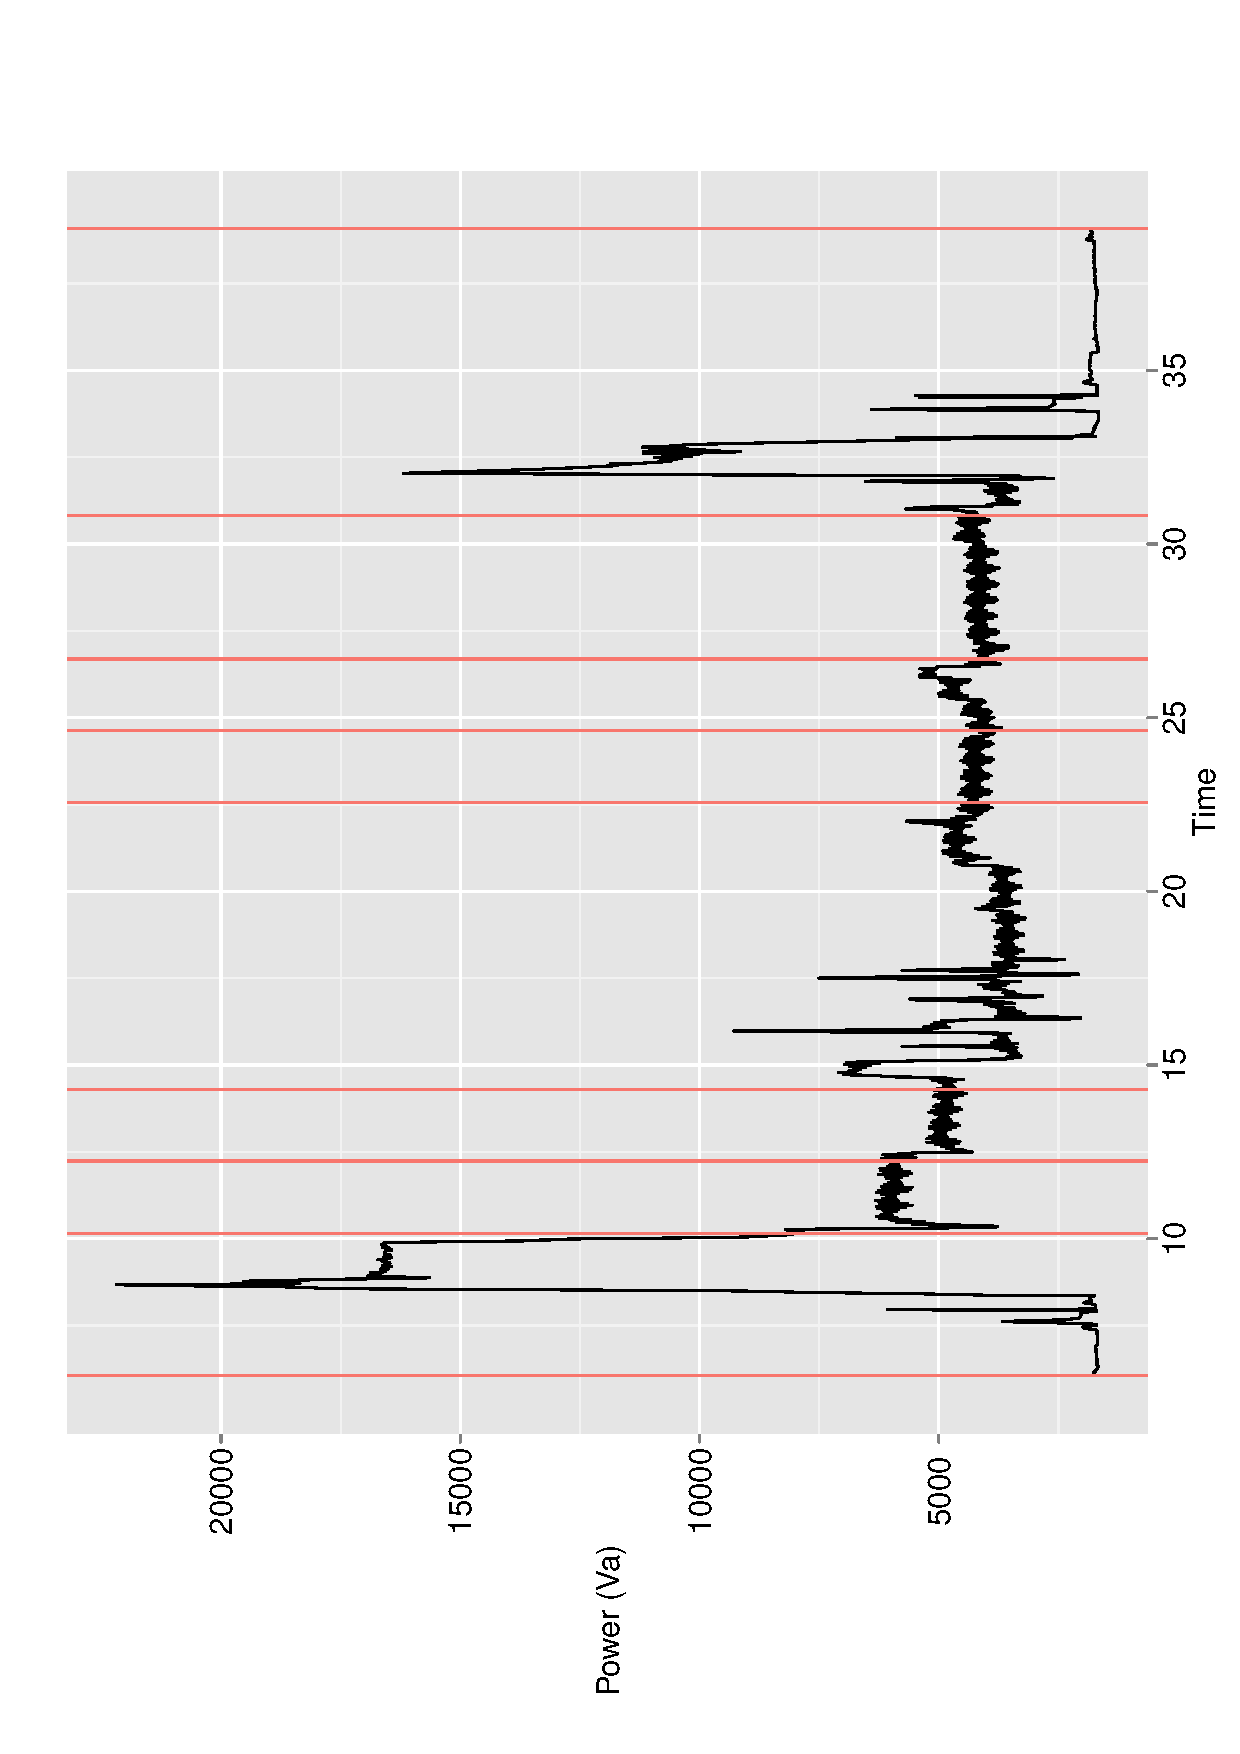
\includegraphics[width=14cm,height=8cm]{Images/1_per_frwd_ortho_split}\caption{Forward feedback splits-Orthonormal variables-1\% relative change
of RMSE threshold-Cycle splits \label{fig:Forward-feedback-splits-Orthonor-1-split}}

\par\end{centering}

\end{figure}


\begin{figure}
\noindent \begin{centering}
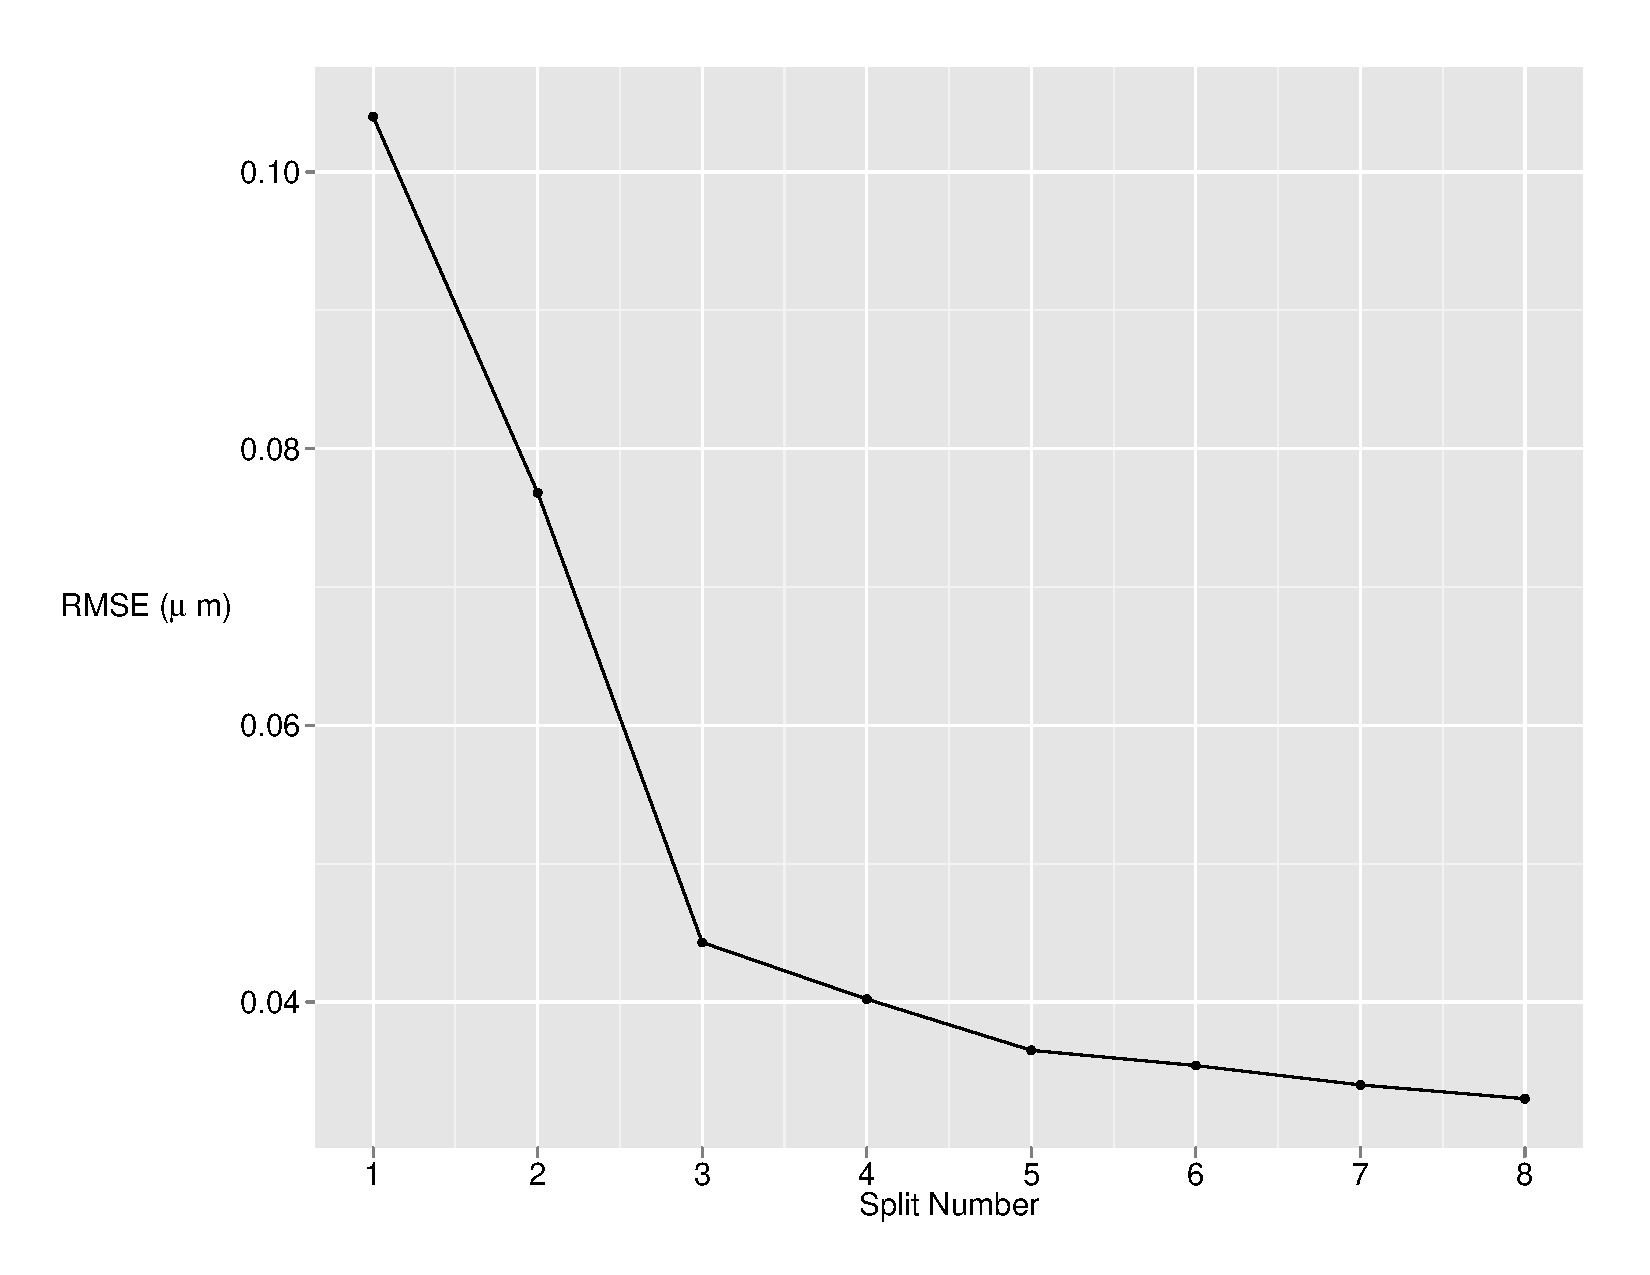
\includegraphics[width=14cm,height=8cm]{Images/1_per_frwd_ortho_err}\caption{Forward feedback splits-Orthonormal variables-1\% relative change
of RMSE threshold-RMSE trend \label{fig:Forward-feedback-splits-Orthonor-1-err}}

\par\end{centering}

\end{figure}


The emergent splits are shown in Fig \ref{fig:Forward-feedback-splits-Orthonor-1-split}
and the RMSE trend can be seen in Fig \ref{fig:Forward-feedback-splits-Orthonor-1-err}.
The final RMSE value is $0.0330\mu m$.


\subsubsection{Reverse feeback splits-Mixed polynomial-5\% relative change of RMSE
threshold}

\begin{figure}
\noindent \begin{centering}
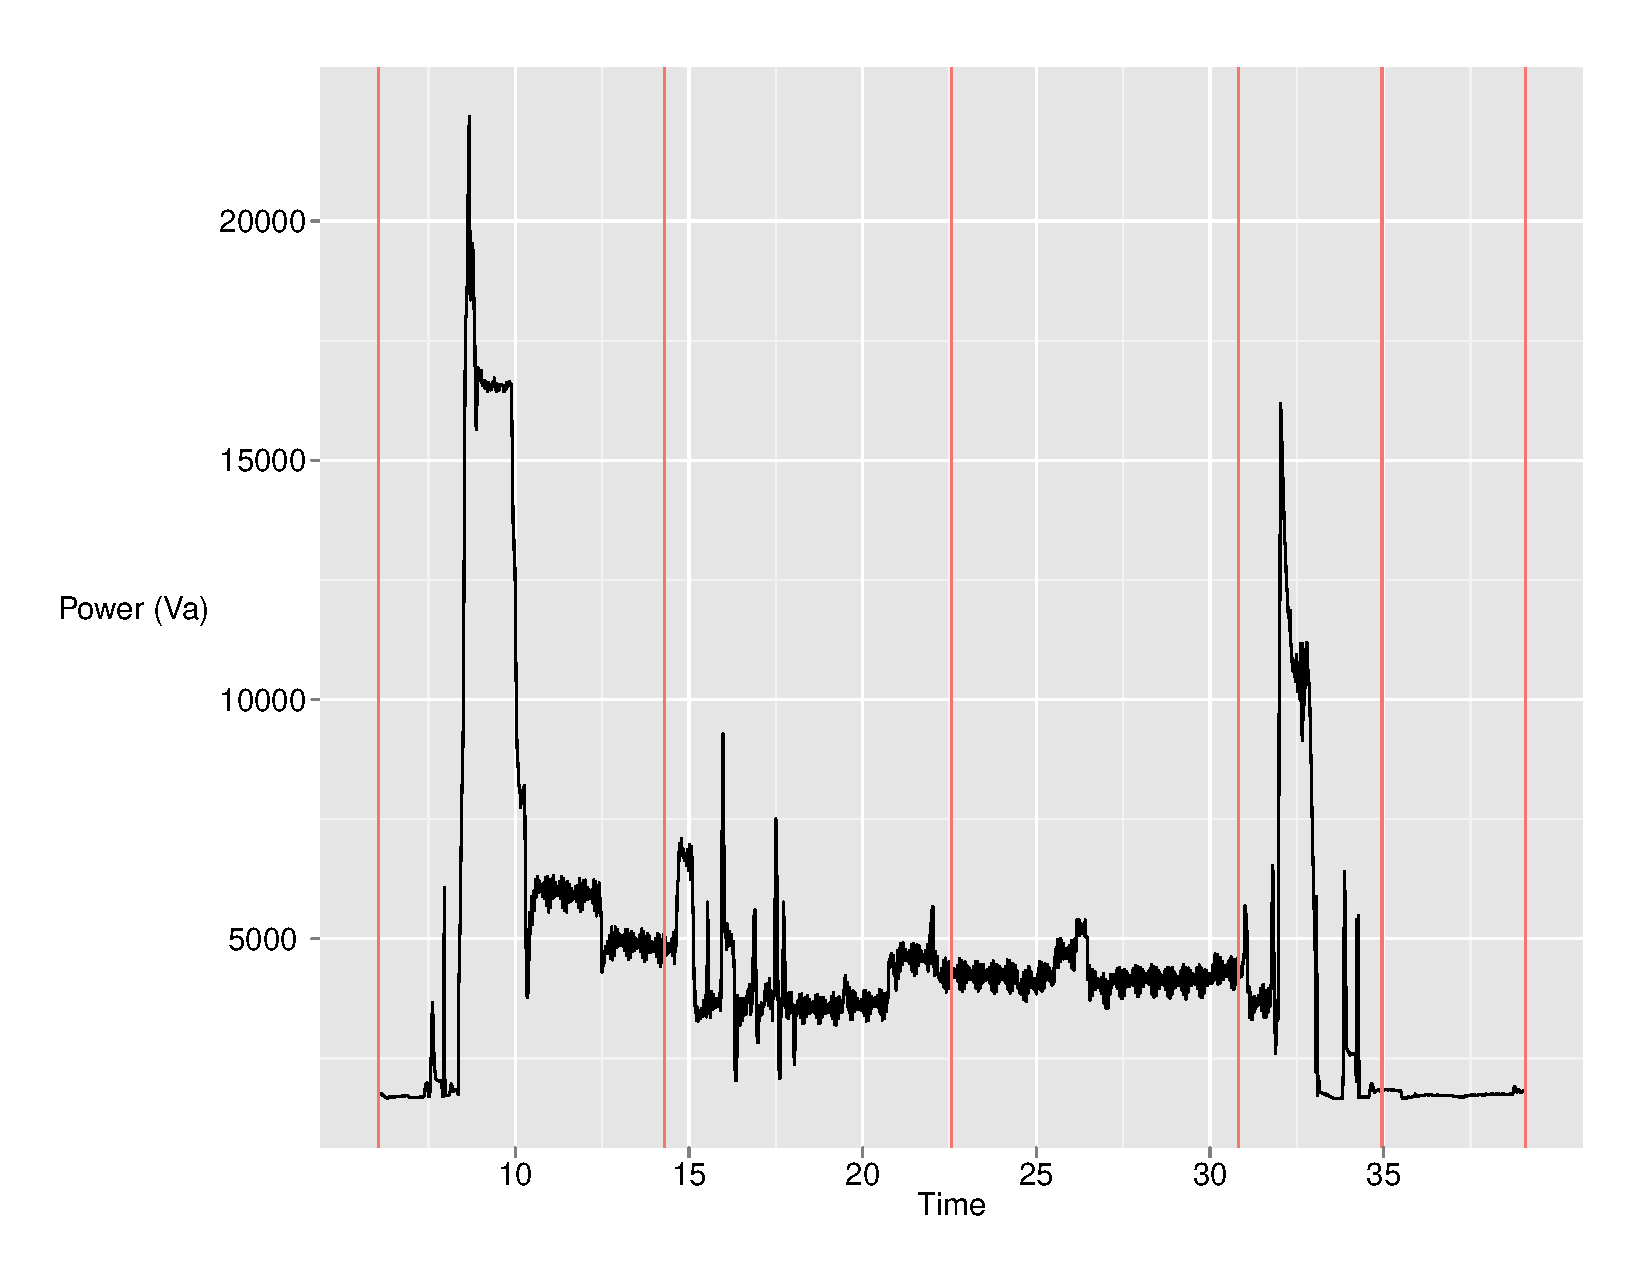
\includegraphics[width=14cm,height=8cm]{Images/5_per_rev_mix_split}\caption{Mixed polynomial reverse feedback splits with 5\% threshold for relative
change in RMSE- Cycle splits \label{fig:Mixed-polynomial-reverse-5-split}}

\par\end{centering}

\end{figure}


\begin{figure}
\noindent \begin{centering}
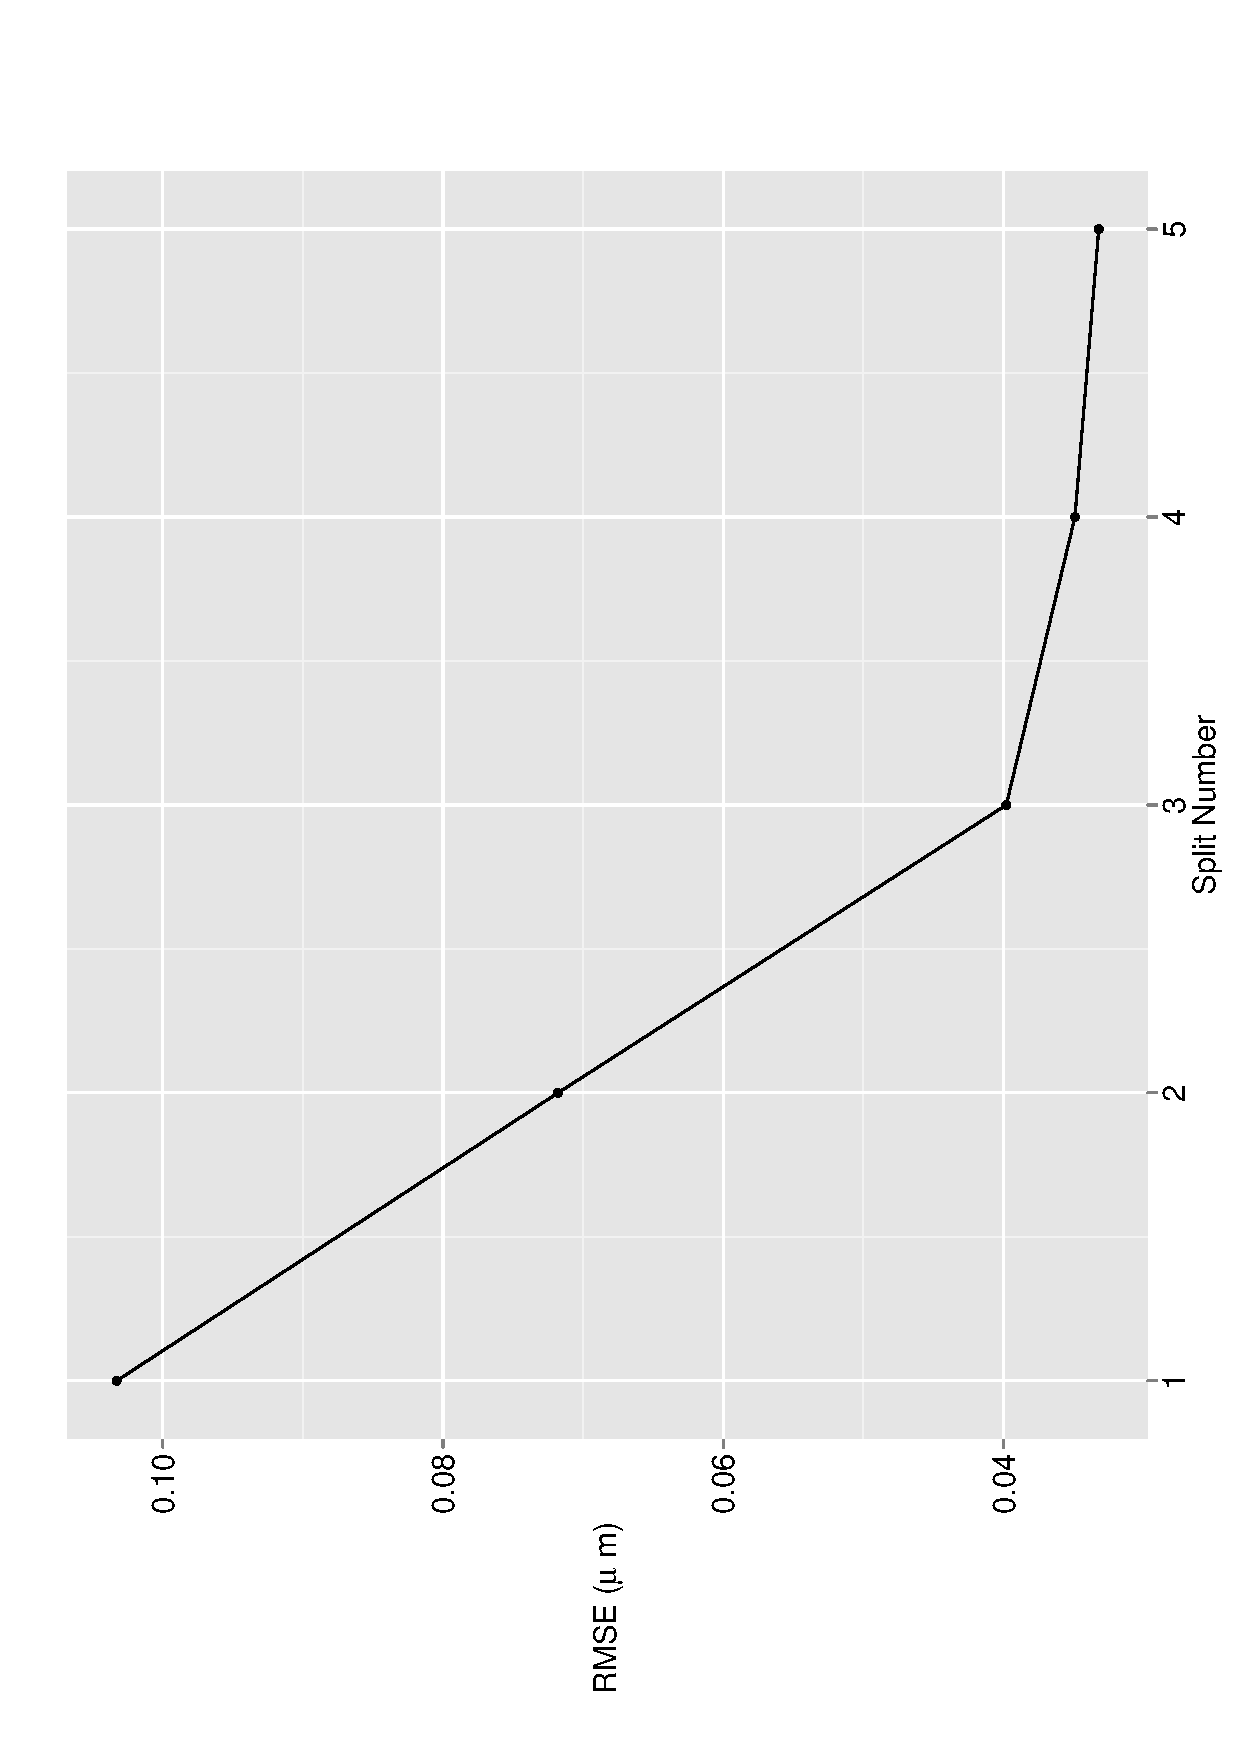
\includegraphics[width=14cm,height=8cm]{Images/5_per_rev_mix_err}\caption{Mixed polynomial reverse feedback splits with 5\% threshold for relative
change in RMSE- RMSE trend \label{fig:Mixed-polynomial-reverse-5-err}}

\par\end{centering}

\end{figure}


The emergent splits are shown in Fig \ref{fig:Forward-feedback-splits-Orthonor-1-split}
and the RMSE trend can be seen in Fig \ref{fig:Forward-feedback-splits-Orthonor-1-err}.
The final RMSE value is $0.0332\mu m$.


\subsubsection{Reverse feeback splits-Orthonormal variable-5\% relative change of
RMSE threshold}

\begin{figure}
\noindent \begin{centering}
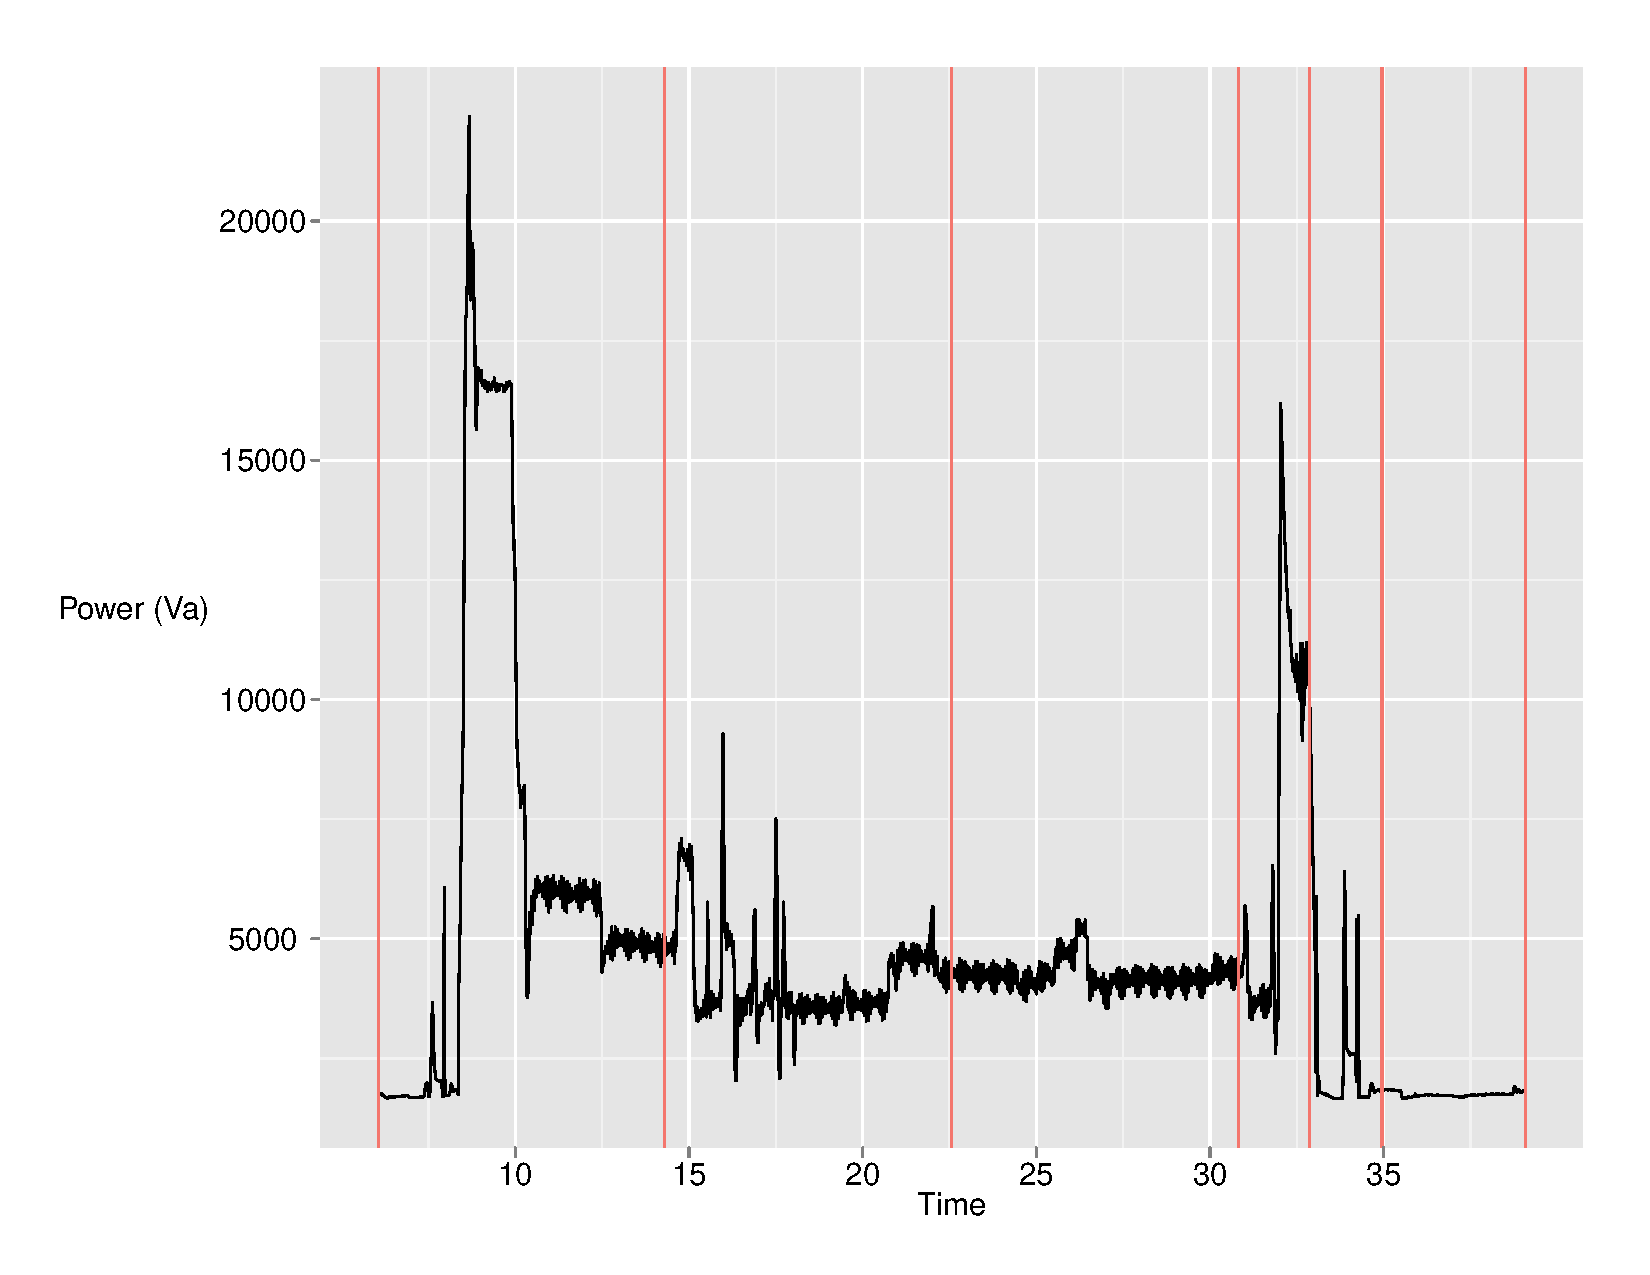
\includegraphics[width=14cm,height=8cm]{Images/5_per_rev_ortho_split}\caption{Reverse feedback splits-Orthonormal variables-5\% relative change
of RMSE threshold - Cycle splits \label{fig:Reverse-feedback-splits-Orthonor-5-split}}

\par\end{centering}

\end{figure}


\begin{figure}
\noindent \begin{centering}
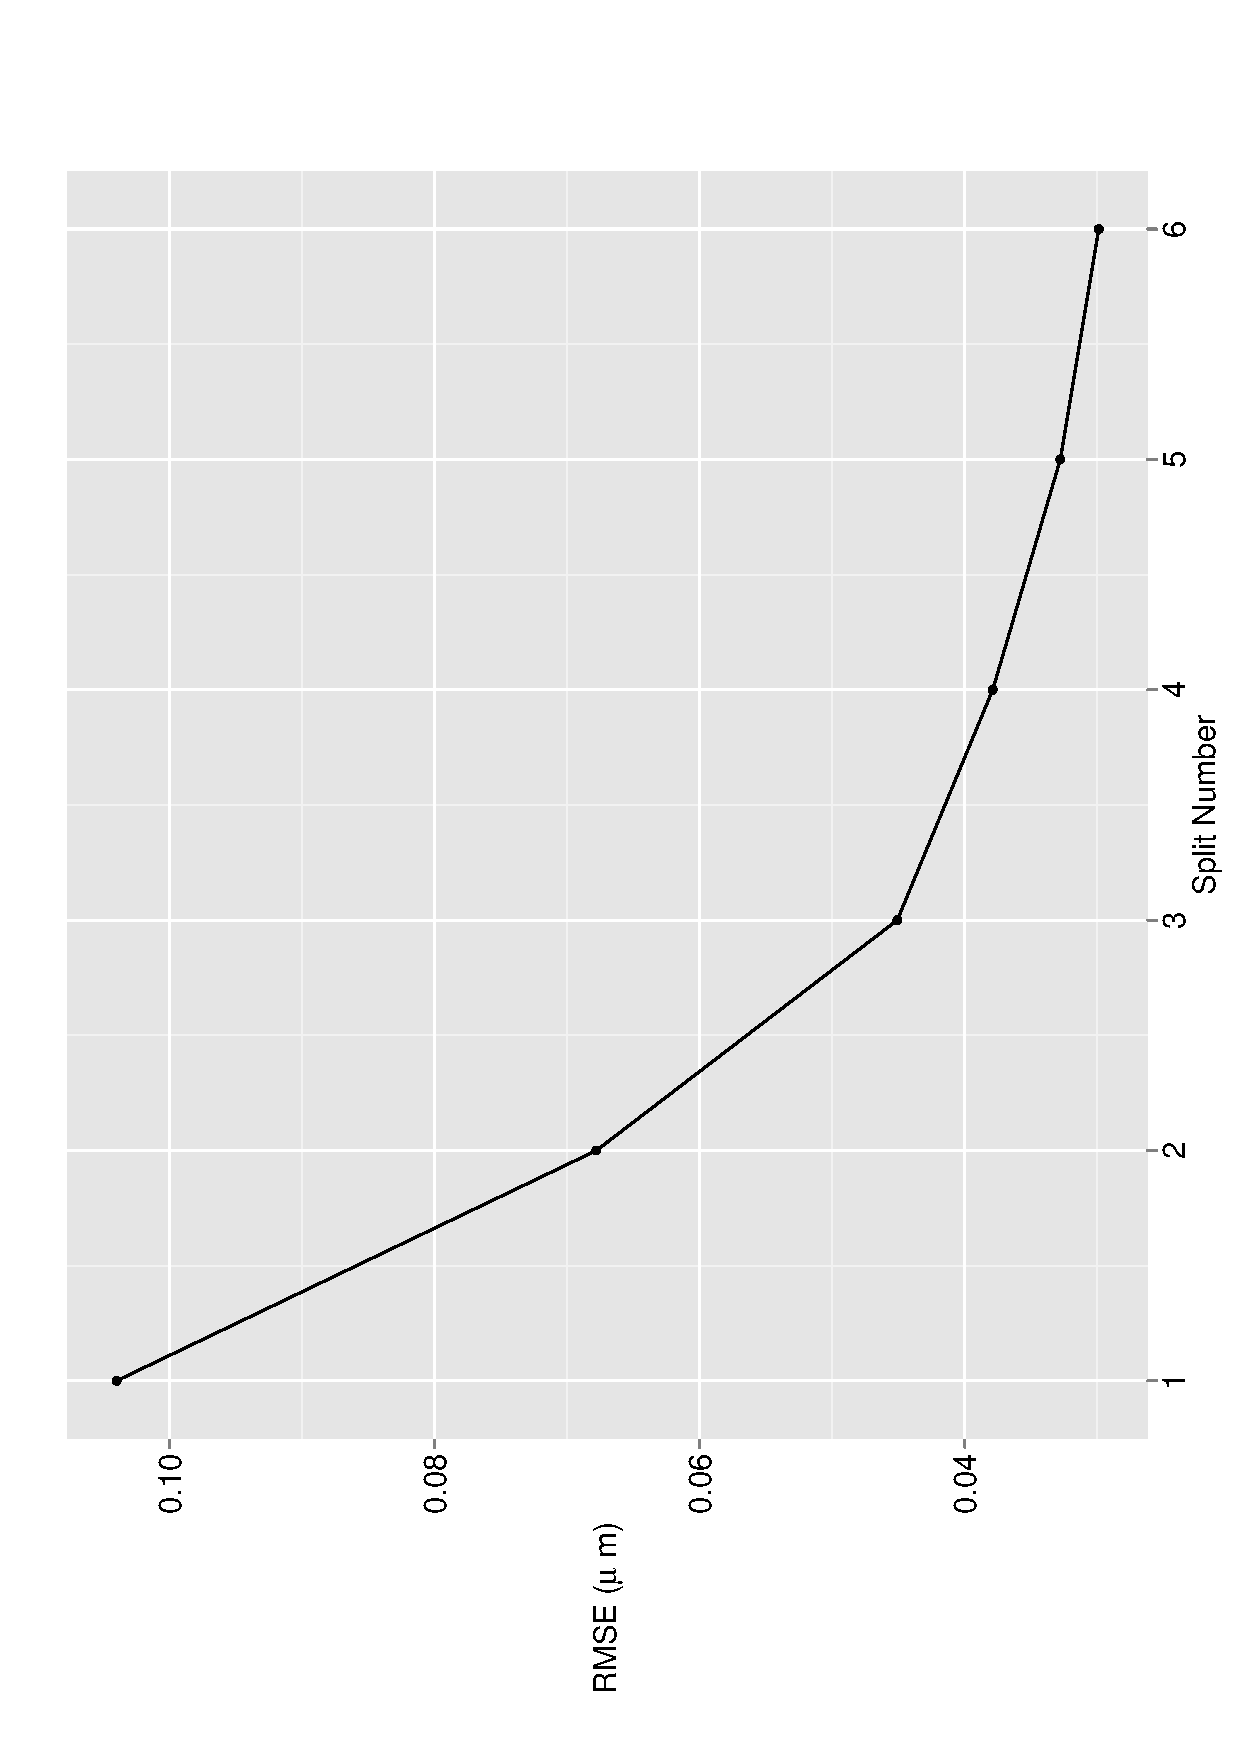
\includegraphics[width=14cm,height=8cm]{Images/5_per_rev_ortho_err}\caption{Reverse feedback splits-Orthonormal variables-5\% relative change
of RMSE threshold - RMSE trend \label{fig:Reverse-feedback-splits-Orthonor-5-err}}

\par\end{centering}

\end{figure}


The emergent splits are shown in Fig \ref{fig:Reverse-feedback-splits-Orthonor-5-split}
and the RMSE trend can be seen in Fig \ref{fig:Reverse-feedback-splits-Orthonor-5-err}.
The final RMSE value is $0.0299\mu m$.


\subsubsection{Reverse feedback splits- Mixed polynomial-1\% relative change of
RMSE threshold}

\begin{figure}
\noindent \centering{}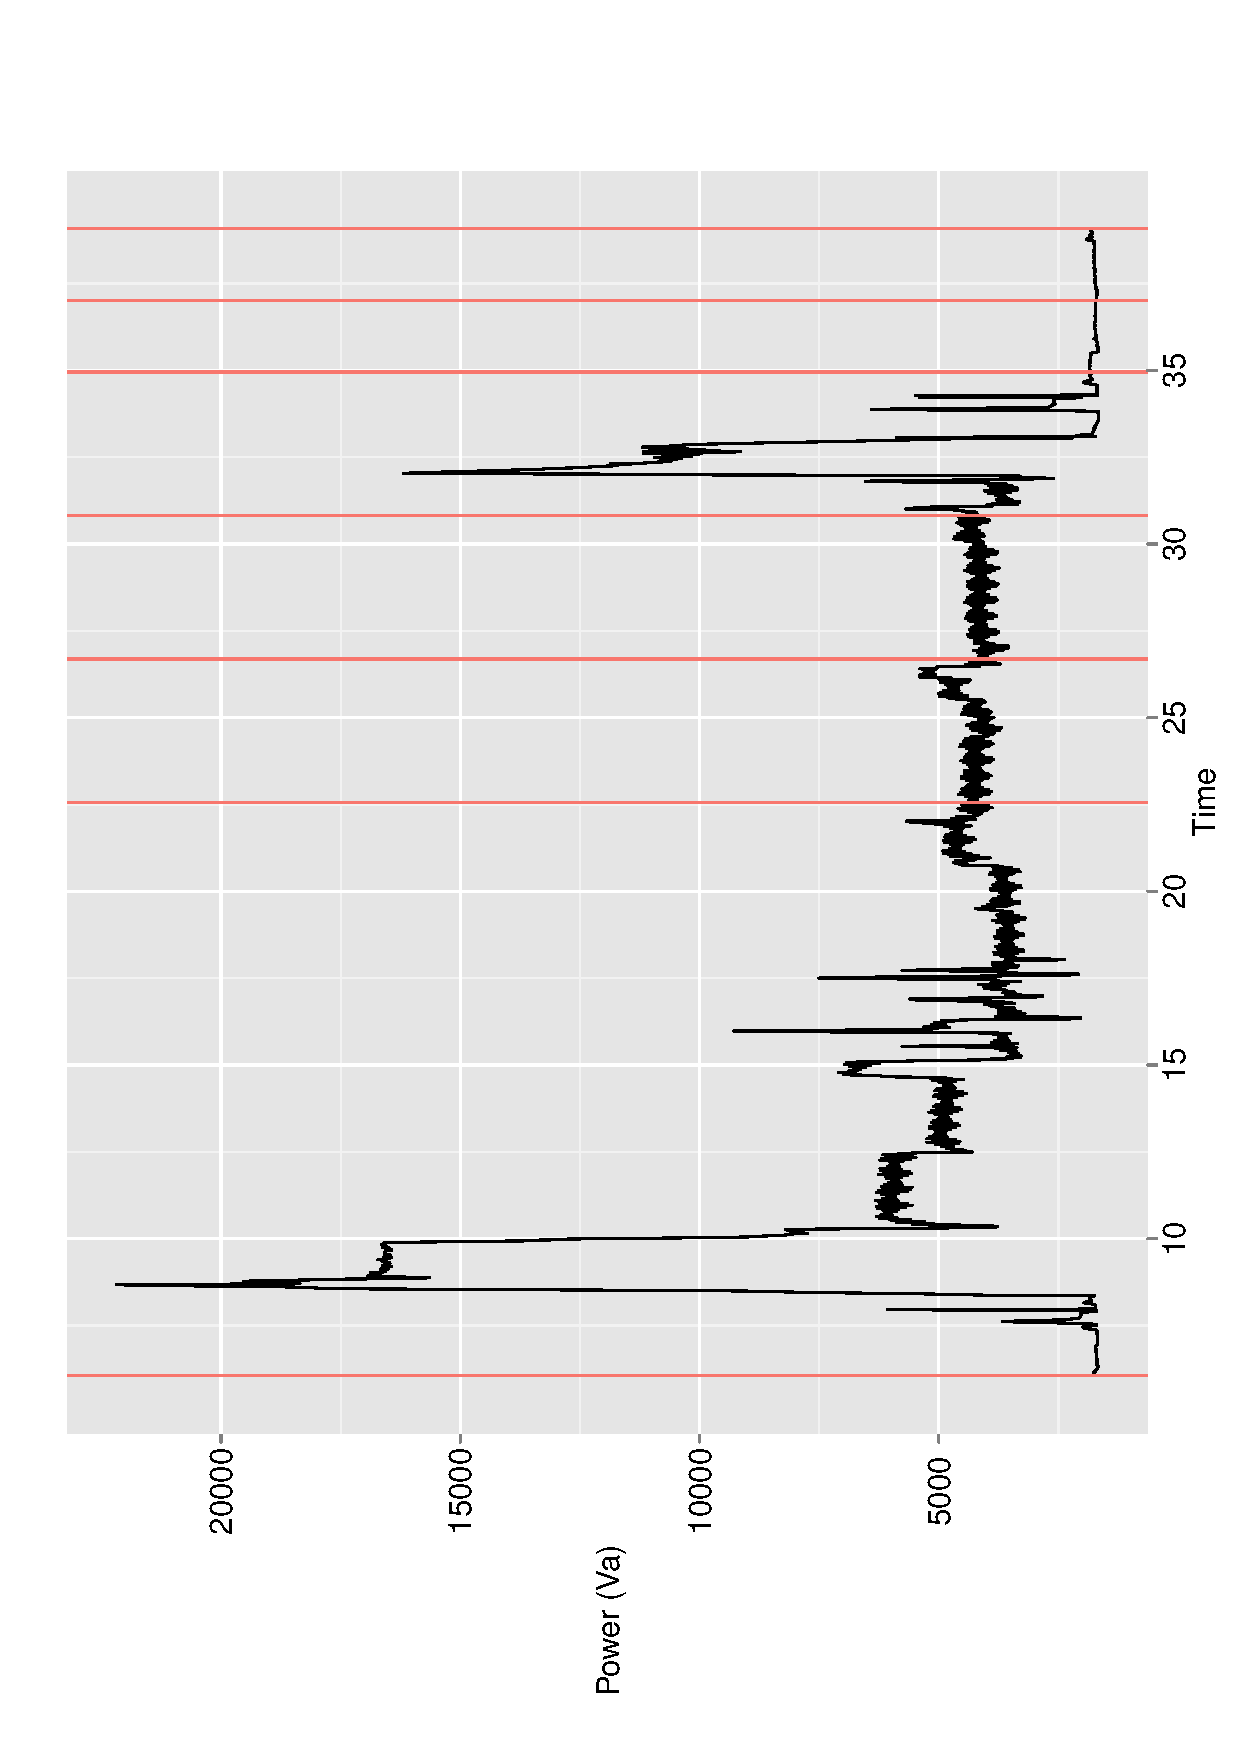
\includegraphics[width=14cm,height=8cm]{Images/1_per_rev_mix_split}\caption{Mixed polynomial reverse feedback splits with 1\% threshold for relative
change in RMSE- Cycle splits \label{fig:Mixed-polynomial-reverse-1-splits}}
\end{figure}


\begin{figure}
\noindent \centering{}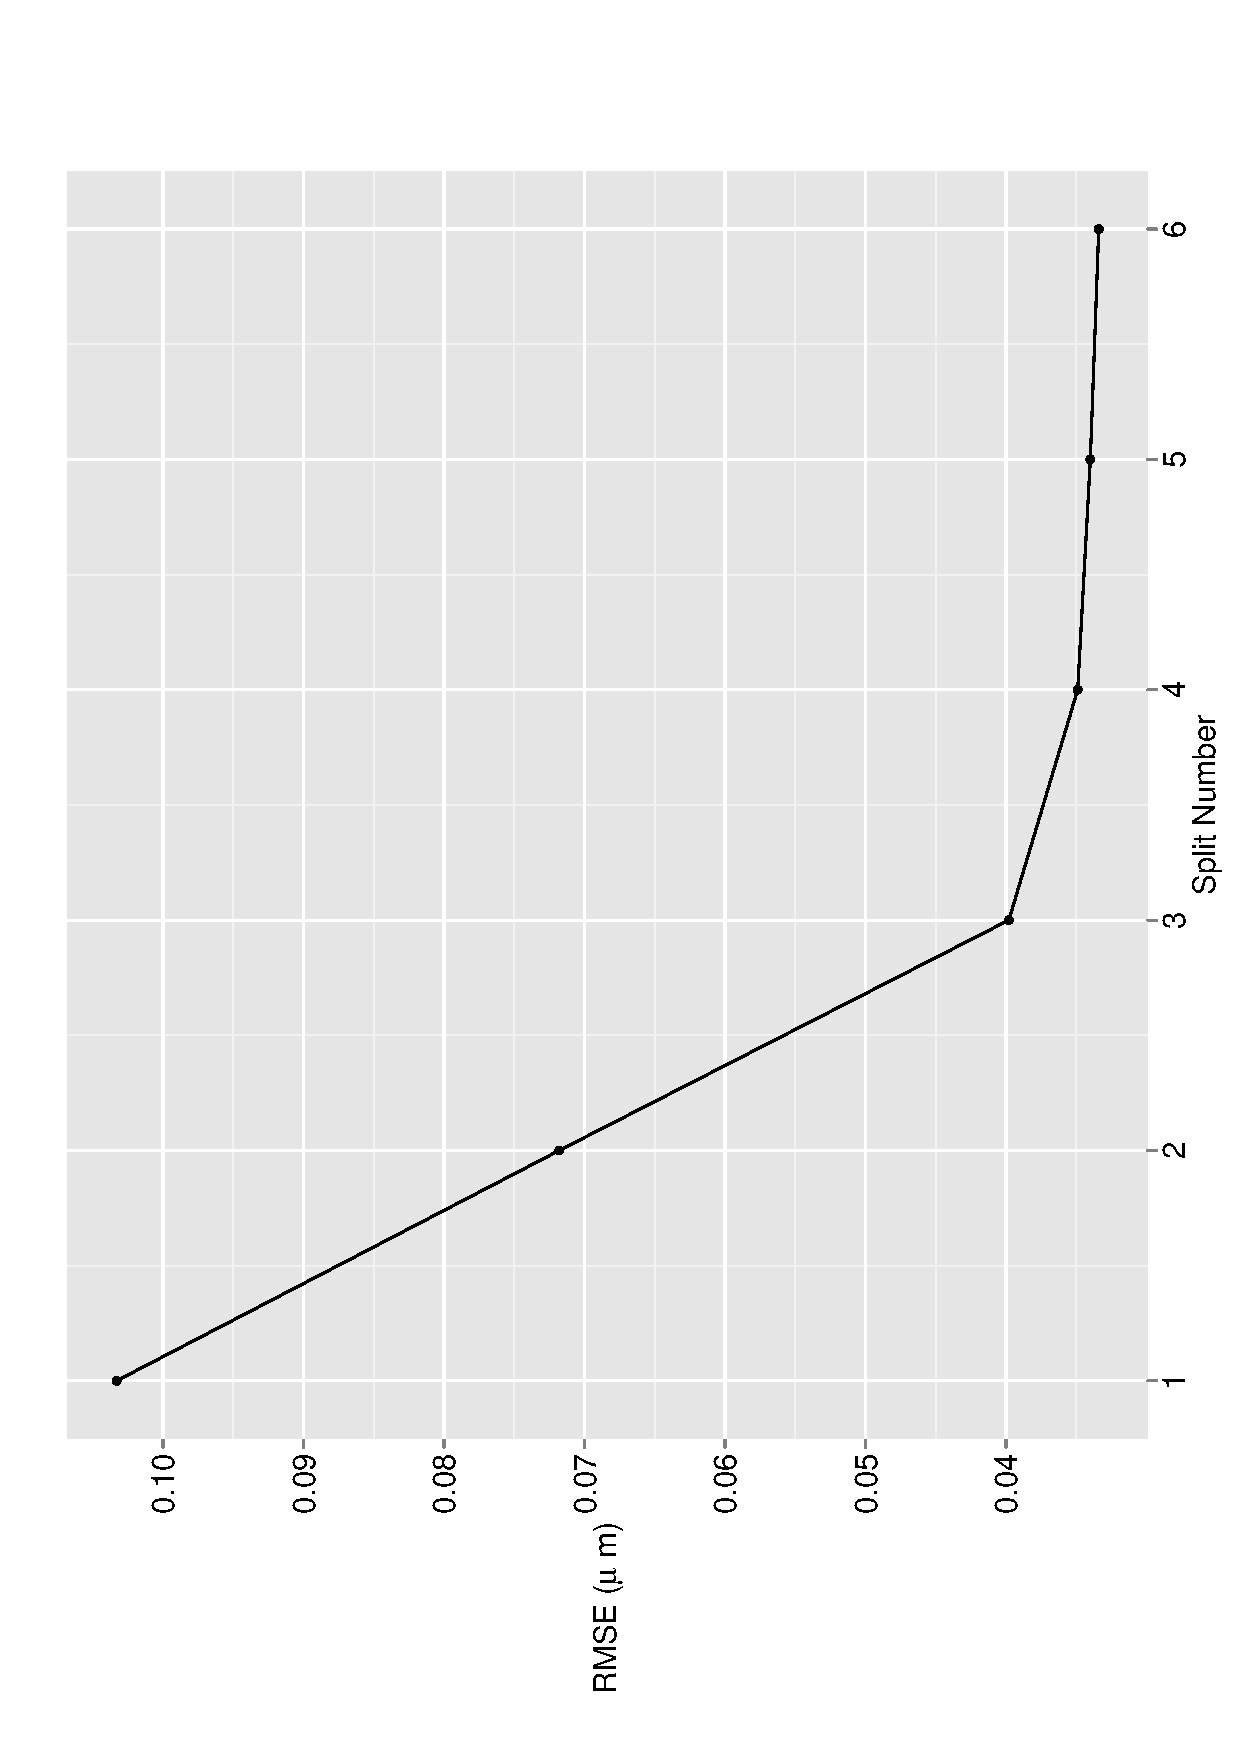
\includegraphics[width=14cm,height=8cm]{Images/1_per_rev_mix_err}\caption{Mixed polynomial reverse feedback splits with 1\% threshold for relative
change in RMSE- RMSE trend \label{fig:Mixed-polynomial-reverse-1-err}}
\end{figure}


The emergent splits are shown in Fig \ref{fig:Mixed-polynomial-reverse-1-splits}
and the RMSE trend can be seen in Fig \ref{fig:Mixed-polynomial-reverse-1-err}.
The final RMSE value is $0.0334\mu m$.


\subsubsection{Reverse feedback splits- Orthonormal variable-1\% relative change
of RMSE threshold}

\begin{figure}
\noindent \centering{}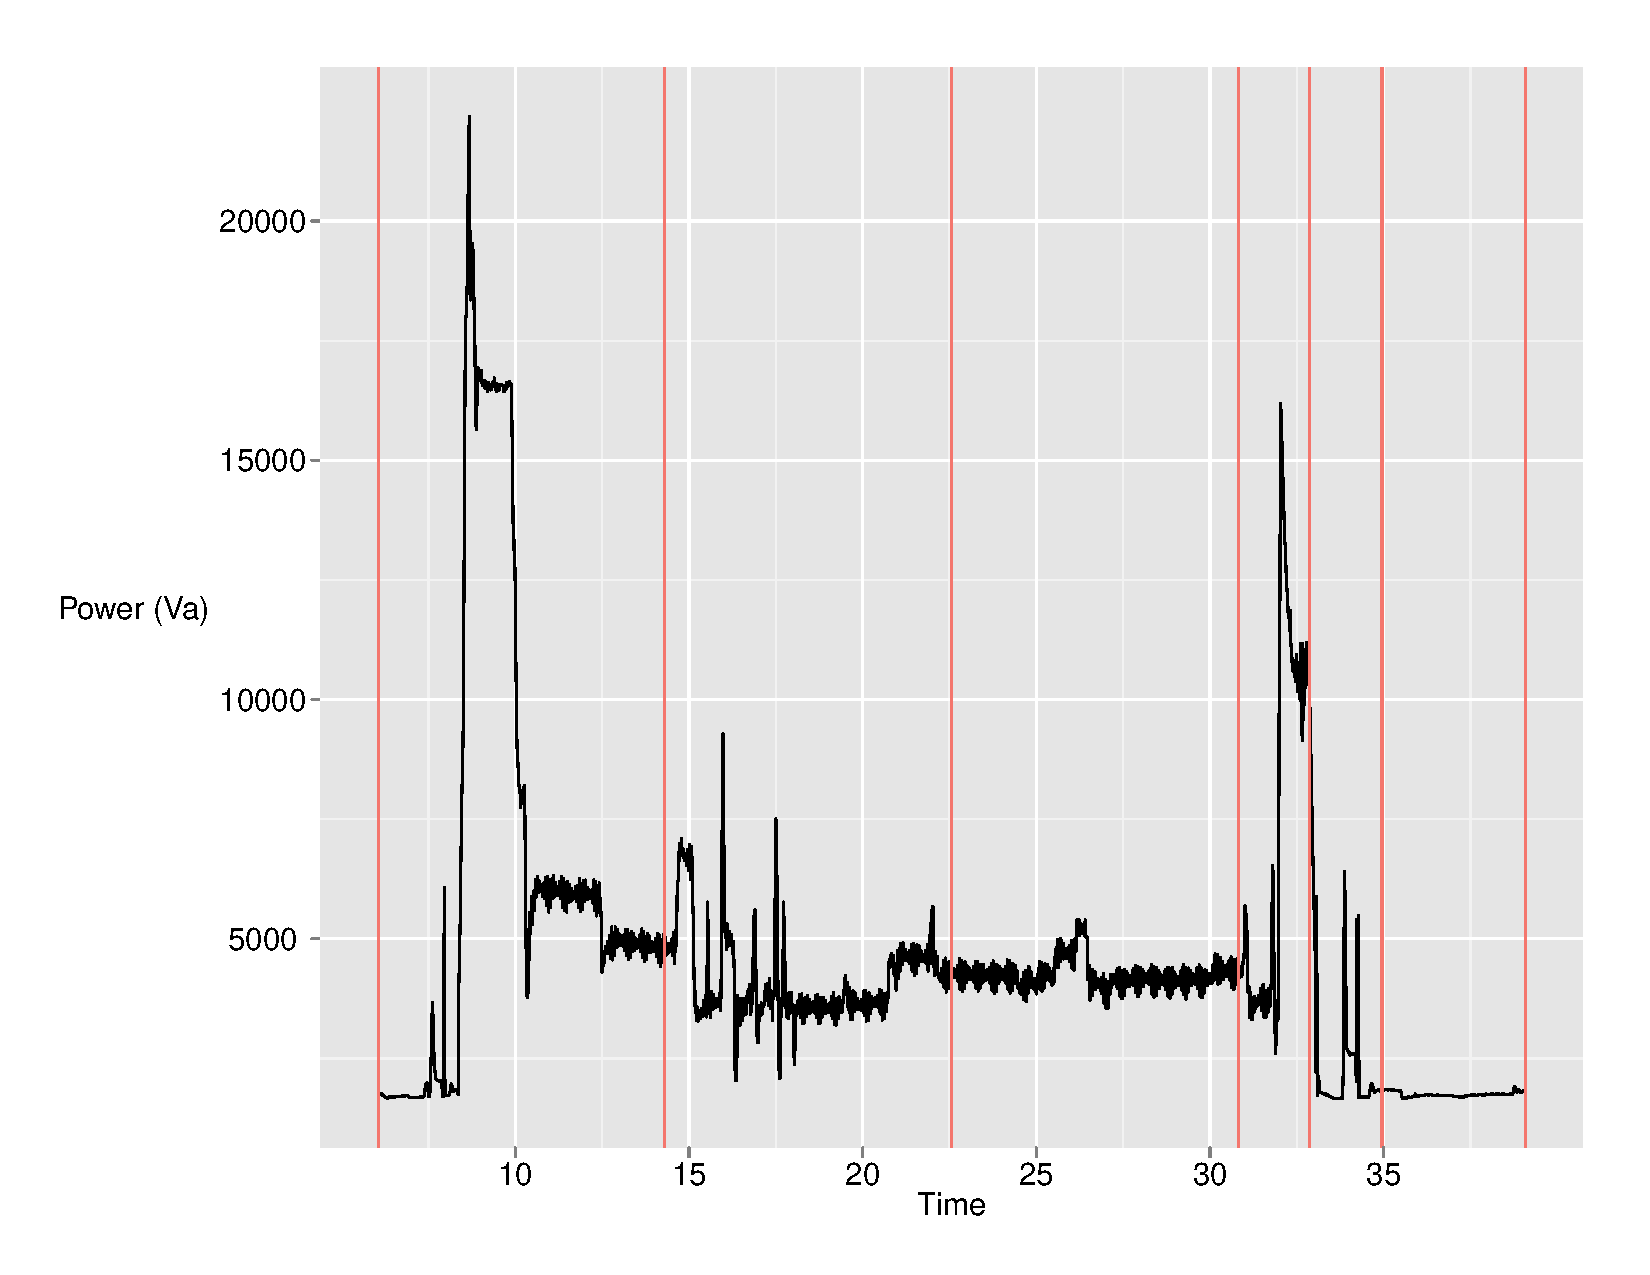
\includegraphics[width=14cm,height=8cm]{Images/1_per_rev_ortho_split}\caption{Reverse feedback splits-Orthonormal variables-1\% relative change
of RMSE threshold- Cyclse splits \label{fig:Reverse-feedback-splits-Orthonor-1-split}}
\end{figure}


\begin{figure}
\noindent \centering{}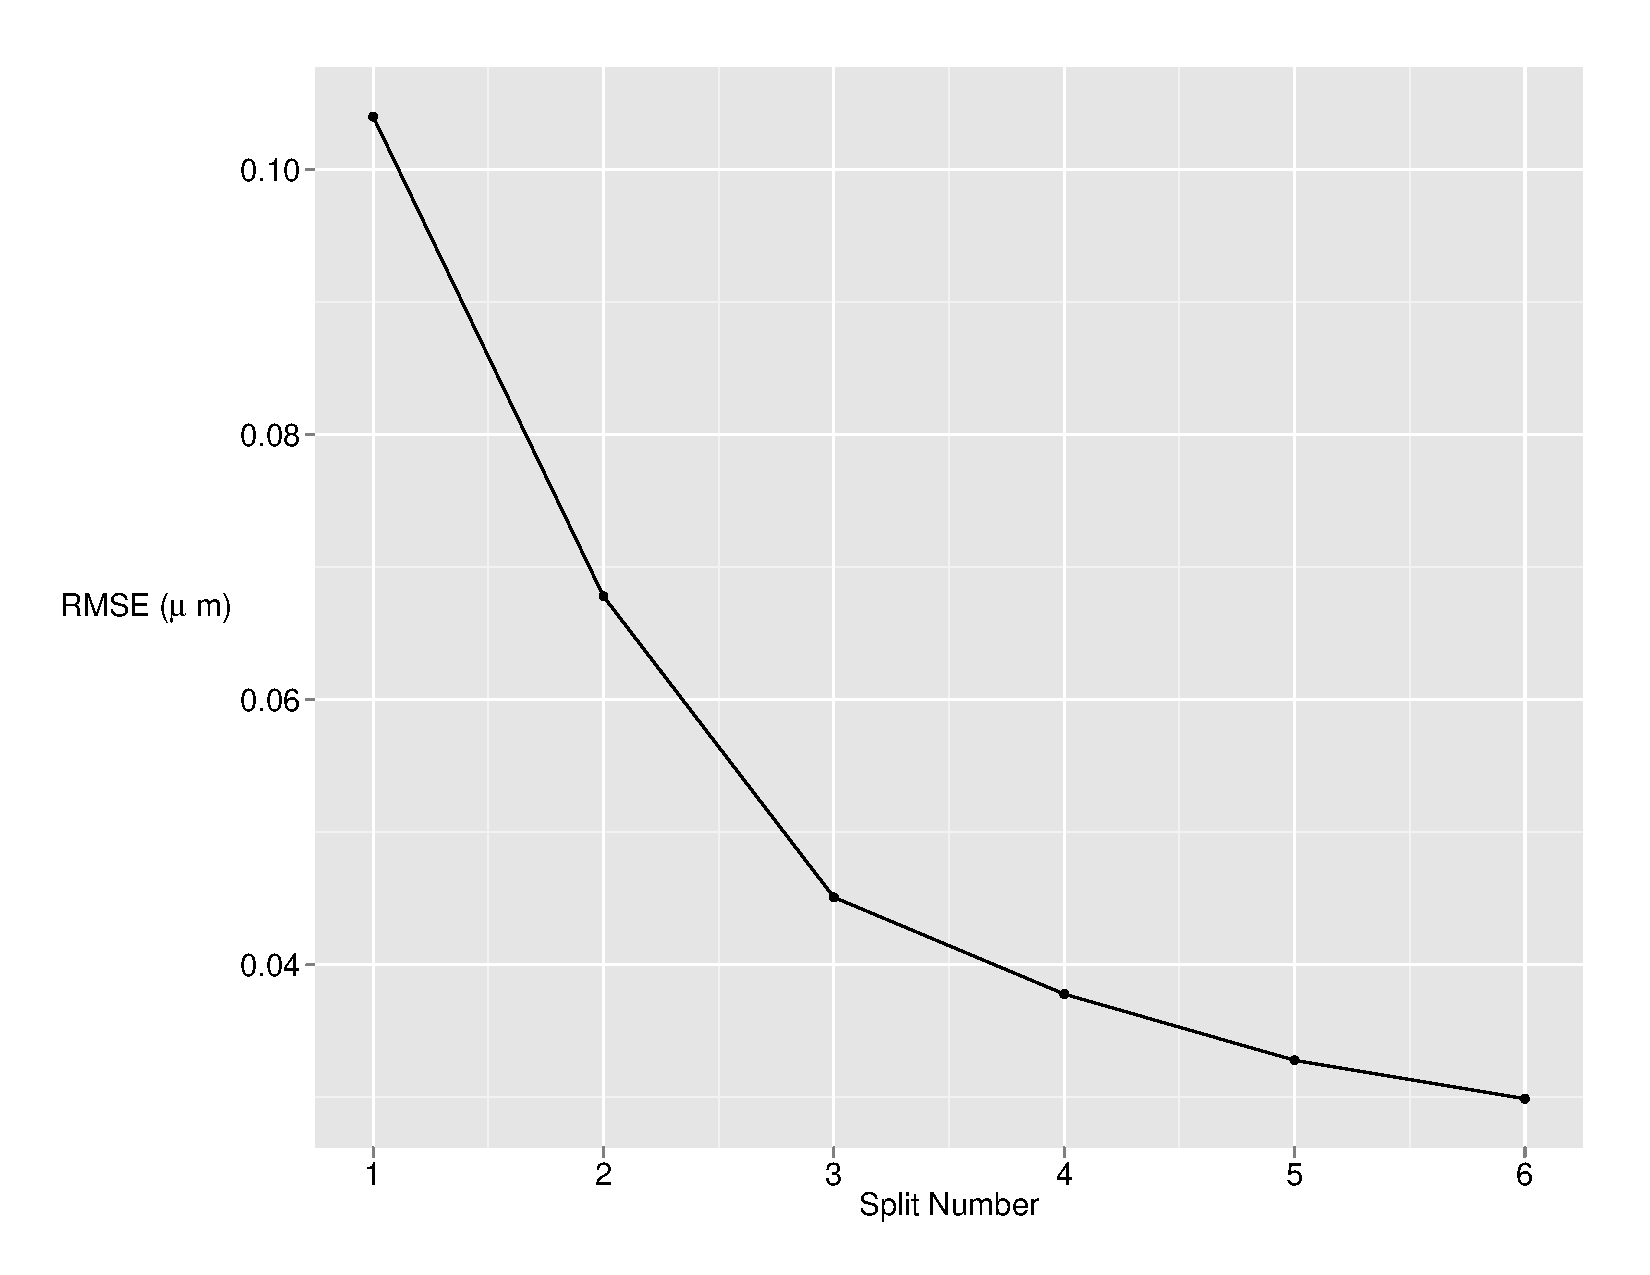
\includegraphics[width=14cm,height=8cm]{Images/1_per_rev_ortho_err}\caption{Reverse feedback splits-Orthonormal variables-1\% relative change
of RMSE threshold- RMSE trend \label{fig:Reverse-feedback-splits-Orthonor-1-err}}
\end{figure}


The emergent splits are shown in Fig \ref{fig:Reverse-feedback-splits-Orthonor-1-split}
and the RMSE trend can be seen in Fig \ref{fig:Reverse-feedback-splits-Orthonor-1-err}.
The final RMSE value is $0.0299\mu m$.


\subsubsection{Discussion }

As we can see from the results above, there isn't a lot of variation
in the final RMSE value which we find using various combinations of
split direction, threshold and variable type. They more or less fall
around $0.03\mu m$. However, there are certain other aspects that
interesting. 
\begin{enumerate}
\item Firstly, as mentioned before, when performing cuts from the start
of the cycle, we tend to get more and closer cuts near the start and
lesser towards the end and the the other way around when we start
splitting from the end of the cycle.
\item Another important thing that we notice is that we get lesser number
of splits when we split from the end of the cycle. This indicates
that we can get better correlation by sampling the end of the cycle.
This inference as mentioned in Section \ref{sub:Discussion-uniform splitting}
is not surprising as the finishing operation is done near the end
of the cycle.
\item As we can see in all the split figures, the significant pattern in
30-35 seconds is considered as section in all of them. In fact, in
reverse splits, better splitting in this region is the reason why
we approach the minimum error region with lesser number of overall
splits.
\end{enumerate}

\subsection{Incremental calculation}

As we would expect while running the algorithm for manually drawn
cuts (ref Section \ref{sub:Cycle-splitting}), the final RMSE values
are more or less the same. However, we tried incremental sectionwise
calculation here. In this, we first include only the first section
as input and find a solution and store the resultant RMSE. Then we
take the first two sections and find a solution ad store the RMSE.
We keep on including subsequent sections and find the correspond RMSE's.
This way we can try to find out the quality of a product before the
part has been finished making. The future applications of such a capability
are immense. Especially for parts which take a lot of time to be machined.

The splits we used for this have been chosen manually as in Fig \ref{fig:Manual-Chosen-splits}. 

\begin{figure}
\noindent \centering{}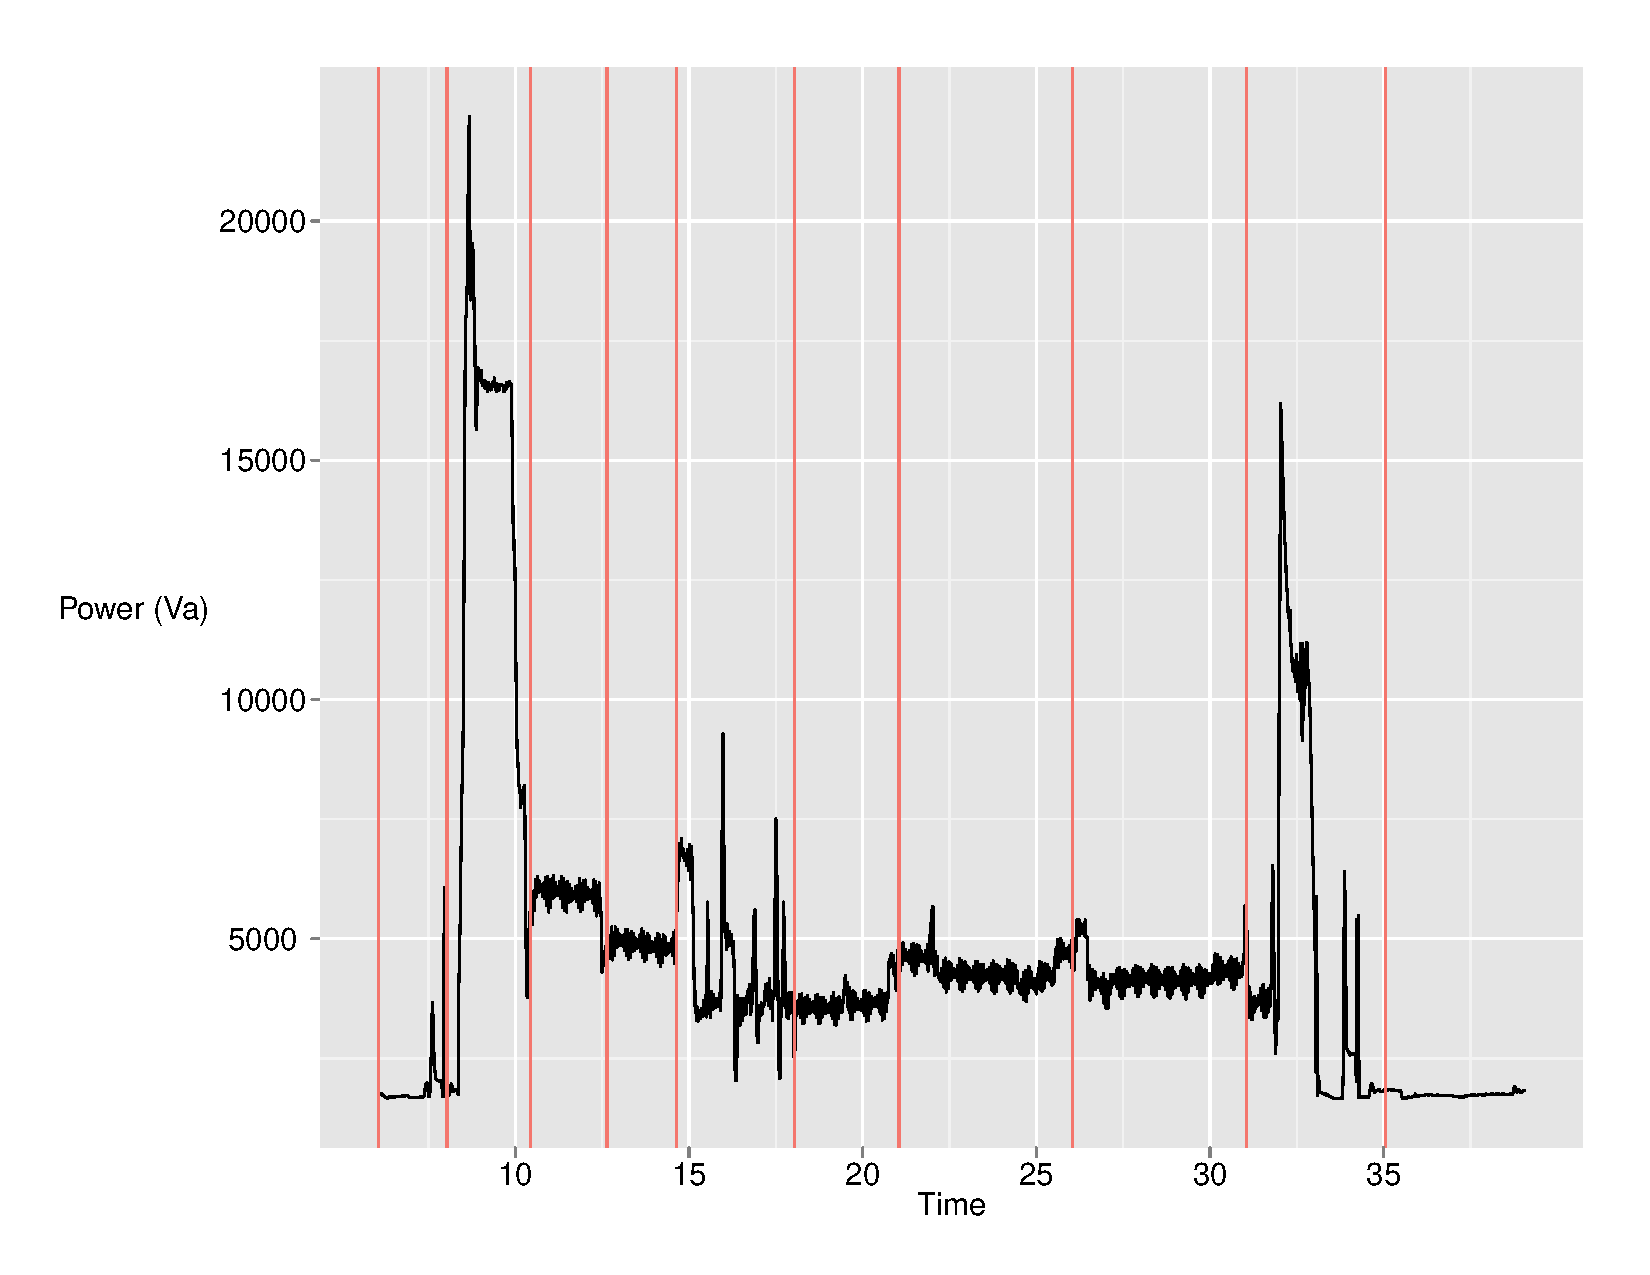
\includegraphics[width=14cm,height=8cm]{Images/manual_split}\caption{Manually Chosen splits \label{fig:Manual-Chosen-splits}}
\end{figure}


As evident from all the previous examples, we don't find significant
variation in the results after using either mixed polynomials or orthogonal
polynomials as our variables. So here we only present the \emph{mixed
polynomial variable }scenario. Also, this scenario will help us in
finding out which sections contribute more to the equation.

In Table \ref{tab:RMSE-values-incremental} we show the RMSE values
we get after using various number of sections from the splits as shown
in Fig \ref{fig:Manual-Chosen-splits} for each degree of the polynomial
variable (mixed polynomial variable). Interestingly we come very close
to to the final RMSE value in the 7th section which ends about 13s
before the end of our cycle (cycle time is 33 sec).

\begin{table}
\noindent \centering{}%
\begin{tabular}{|>{\centering}p{1cm}|>{\centering}p{1cm}|>{\centering}p{1cm}|>{\centering}p{1cm}|>{\centering}p{1cm}|>{\centering}p{1cm}|>{\centering}p{1cm}|>{\centering}p{1cm}|>{\centering}p{1cm}|>{\centering}p{1cm}|>{\centering}p{1cm}|}
\hline 
\multicolumn{1}{|>{\centering}p{1cm}|}{} & After 1 section & After 2 sections & After 3 sections & After 4 sections & After 5 sections & After 6 sections & After 7 sections & After 8 sections & After 9 sections & After 10 sections\tabularnewline
\hline 
\hline 
Degree 2 polynomial & 0.1126 & 0.1125 & 0.0947 & 0.0668 & 0.0608 & 0.0542 & 0.0332 & 0.0329 & 0.0329 & 0.0321\tabularnewline
\hline 
Degree 3 polynomial & 0.1132 & 0.1120 & 0.0902 & 0.0665 & 0.0603 & 0.0570 & 0.0338 & 0.0315 & 0.0318 & 0.0317\tabularnewline
\hline 
Degree 4 polynomial & 0.1264 & 0.1274 & 0.0901 & 0.0678 & 0.0606 & 0.0563 & 0.0329 & 0.0304 & 0.0282 & 0.0301\tabularnewline
\hline 
Degree 5 polynomial & 0.1251 & 2.1440 & 0.0942 & 0.0661 & 0.0600 & 0.0533 & 0.0320 & 0.0291 & 0.0285 & 0.0283\tabularnewline
\hline 
\end{tabular}\caption{RMSE values (in $\mu m$) for Incremental error calculation \label{tab:RMSE-values-incremental}}
\end{table}


\begin{table}
\noindent \begin{centering}
\begin{tabular}{|>{\centering}p{2cm}|>{\centering}p{2cm}|>{\centering}p{2cm}|}
\hline 
Minimum value of variable & Value of coefficient & Maximum value of variable\tabularnewline
\hline 
\hline 
1.00E-15 & 3.08E+15 & 1.00E-15\tabularnewline
\hline 
4.78E-03 & 4.81E-09 & 1.62E+03\tabularnewline
\hline 
1.96E-09 & 4.16E-04 & 2.81E-04\tabularnewline
\hline 
7.01E-06 & 6.26E-04 & 1.72E-01\tabularnewline
\hline 
5.72E-04 & 1.10E-03 & 2.90E+01\tabularnewline
\hline 
1.30E+02 & 1.93E-04 & 3.37E+02\tabularnewline
\hline 
3.65E-12 & 6.87E-05 & 4.43E-12\tabularnewline
\hline 
2.05E+02 & 6.74E-08 & 7.01E+02\tabularnewline
\hline 
1.31E+02 & 1.02E-03 & 3.11E+02\tabularnewline
\hline 
9.70E+02 & 9.51E-05 & 4.54E+03\tabularnewline
\hline 
1.90E+02 & 1.21E-04 & 7.02E+02\tabularnewline
\hline 
1.33E+02 & 2.43E-03 & 2.90E+02\tabularnewline
\hline 
1.77E+02 & 7.68E-09 & 7.03E+02\tabularnewline
\hline 
1.04E-09 & -1.81E+10 & 1.58E-08\tabularnewline
\hline 
3.91E-06 & -7.74E+05 & 6.12E-05\tabularnewline
\hline 
1.47E-02 & -1.45E+02 & 2.37E-01\tabularnewline
\hline 
5.53E+01 & -3.07E-02 & 9.20E+02\tabularnewline
\hline 
4.45E-12 & -6.99E-06 & 5.40E-12\tabularnewline
\hline 
4.50E+01 & -2.31E-03 & 9.93E+01\tabularnewline
\hline 
8.42E-03 & -7.55E-04 & 2.02E-02\tabularnewline
\hline 
3.23E+01 & -3.00E-06 & 7.83E+01\tabularnewline
\hline 
1.10E+02 & -8.88E-05 & 2.96E+03\tabularnewline
\hline 
1.48E+01 & -5.65E-04 & 8.07E+01\tabularnewline
\hline 
2.01E+01 & -1.10E-04 & 5.77E+02\tabularnewline
\hline 
1.05E+02 & -1.72E-05 & 7.06E+02\tabularnewline
\hline 
2.59E-09 & 7.60E-06 & 5.86E-09\tabularnewline
\hline 
8.88E-05 & 2.24E-02 & 2.15E-04\tabularnewline
\hline 
1.08E-05 & 5.80E-06 & 2.40E-05\tabularnewline
\hline 
1.09E-05 & 5.62E-09 & 2.36E-05\tabularnewline
\hline 
2.62E-08 & 1.09E-05 & 5.20E-08\tabularnewline
\hline 
2.23E-08 & -2.28E-01 & 5.07E-07\tabularnewline
\hline 
5.51E+01 & -3.50E-06 & 1.87E+04\tabularnewline
\hline 
7.52E+02 & -1.26E-05 & 4.35E+03\tabularnewline
\hline 
1.70E-05 & 2.78E-04 & 3.79E-04\tabularnewline
\hline 
4.60E+01 & -5.29E-04 & 1.00E+02\tabularnewline
\hline 
3.57E+01 & -2.49E-03 & 7.77E+01\tabularnewline
\hline 
5.53E-06 & 2.93E-06 & 1.12E-05\tabularnewline
\hline 
\end{tabular}
\par\end{centering}

\caption{Table of coefficients for Incremental error calculation \label{tab:Table-of-coefficients}}
\end{table}


Table \ref{tab:Table-of-coefficients} shows a particular solutions'
(Degree 5 polynomial with 10 sections) statistics. The middle column
shows the list of coefficients in the equation we get. Columns 1 and
3 show the minimum and maximum value of the variables that we get
using the test set for that corresponding variable. When we look at
the coefficients we find that the 14th coefficient is the highest.
Infact the order of magnitude of the product of fourteenth variable
with it's corresponding coefficient is the highest too. Thus, clearly,
these variables can be told to be the most important variables. If
we denote this variable as $x_{imp},$ it turns out that this variable
is given as;
\[
x_{imp}=sd(sec_{9})*sd(sec_{10})
\]


where $sd()$ is the standard deviation function and $sec_{x}$ denotes
section number $x$. Thus we again see that the end of the cycle is
the region which gives us the most important information.

\appendix

\section{Appendix name}

Appendix, only when needed.


\section*{-----------------}

You can use either Bib\TeX{}:

\bibliographystyle{elsarticle-harv}
\addcontentsline{toc}{section}{\refname}\bibliography{../examples/biblioExample}



\section*{---------------------}

\noindent Or plain bibliography:
\begin{thebibliography}{References}
\bibitem{key-1}Frank Mittelbach and Michel Goossens: \emph{The \LaTeX{}
Companion Second Edition.} Addison-Wesley, 2004.

\bibitem{key-2}Scott Pakin. The comprehensive \LaTeX{} symbol list,
2005.\end{thebibliography}

\end{document}
